%template taken from
%University of Bonn Master of Life Science Informatics
% arara: pdflatex: { synctex: on }

\documentclass[twoside, 12pt,  footinclude=true,  headinclude=true,  cleardoublepage=empty]{scrbook}

\usepackage[utf8]{inputenc}
\usepackage [english] {babel}

\usepackage[]{biblatex}
\addbibresource{references.bib}

\usepackage{lipsum}
\usepackage[linedheaders,parts,pdfspacing]{classicthesis}
\usepackage{amsmath}
\usepackage{amsthm}
\usepackage{booktabs}
\usepackage{graphicx}
\usepackage{float}
\usepackage{indentfirst}
\usepackage [T1]{fontenc}
\usepackage{listings}
\usepackage{color}
\usepackage{multirow}
\usepackage{tikz}
\usepackage[toc,page]{appendix}
\usepackage{MnSymbol}
\usepackage{longtable}
\usepackage{graphicx}
\usepackage{subcaption}
\usepackage{mathtools}
\usepackage{enumerate}
\usepackage{csquotes}
\usepackage{amsmath}
\usepackage{hyperref}
\usepackage{acro}
\usepackage[a4paper,includeall,bindingoffset=20mm,margin=2cm,marginparsep=0cm,marginparwidth=0cm]{geometry}
\usepackage[font={footnotesize,it}, labelfont=bf]{caption}

\DeclareAcronym{AD}{
	short = AD ,
	long  = Alzheimer's disease
}
\DeclareAcronym{API}{
	short = API ,
	long  = Application Programming Interface
}
\DeclareAcronym{BioPAX}{
	short = BioPAX,
	long  = Biological Pathway Exchange Language
}
\DeclareAcronym{BEL}{
	short = BEL,
	long  = Biological Expression Language
}
\DeclareAcronym{BELIEF}{
	short = BELIEF,
	long  = Biological Expression Language Information Extraction Workflow
}
\DeclareAcronym{BRENDA}{
	short = BRENDA,
	long  = Braunschweig Enzyme Database
}
\DeclareAcronym{ChEBI}{
	short = ChEBI,
	long  = Chemical Entities of Biological Interest
}
\DeclareAcronym{CI}{
	short = CI,
	long  = Continuous Integration
}
\DeclareAcronym{CSV}{
	short = CSV,
	long  = Comma Separated Values
}
\DeclareAcronym{DL}{
	short = DL,
	long  = Descriptive Logic
}
\DeclareAcronym{eQTL}{
	short = eQTL,
	long  = Expression Quantitative Trait Loci
}
\DeclareAcronym{eSNPO}{
	short = eSNPO,
	long  = eQTL Single Nucleotide Polymorphism Ontology
}
\DeclareAcronym{FCS}{
	short = FCS,
	long  = Functional Class Scoring
}
\DeclareAcronym{GML}{
	short = GML,
	long  = Graph Markup Language
}
\DeclareAcronym{GO}{
	short = GO,
	long  = Gene Ontology
}
\DeclareAcronym{GraphQL}{
	short = GraphQL,
	long  = Graph Query Language
}
\DeclareAcronym{GRP}{
	short = GRP,
	long  = Gene Set File Format
}
\DeclareAcronym{GSEA}{
	short = GSEA,
	long  = Gene Set Enrichment Analysis
}
\DeclareAcronym{HGNC}{
	short = HGNC,
	long  = HUGO Gene Nomenclature Committee
}
\DeclareAcronym{HTML}{
	short = HTML,
	long  = HyperText Markup Language
}
\DeclareAcronym{HUGO}{
	short = HUGO,
	long  = Human Genome Organization
}
\DeclareAcronym{IMI}{
	short = IMI,
	long  = International Medicine Initiative
}
\DeclareAcronym{INDRA}{
	short = INDRA,
	long  = Integrated Dynamical Reasoner and Assembler
}
\DeclareAcronym{IRI}{
	short = IRI,
	long  = Internationalized Resource Identifier
}
\DeclareAcronym{JGIF}{
	short = JFIG,
	long  = JSON Graph Interchange Format
}
\DeclareAcronym{JSON}{
	short = JSON,
	long  = JavaScript Object Notation
}
\DeclareAcronym{JSONLD}{
	short = JSON-LD,
	long  = JSON Linked Data
}
\DeclareAcronym{KEGG}{
	short = KEGG,
	long  = Kyoto Encyclopedia of Genes and Genomes
}
\DeclareAcronym{MeSH}{
	short = MeSH,
	long  = Medical Subject Headings
}
\DeclareAcronym{NDEx}{
	short = NDEx,
	long  = Network Data Exchange
}
\DeclareAcronym{NeuroMMSig}{
	short = NeuroMMSig,
	long  = Multimodal Mechanistic Signatures for Neurodegenerative Diseases
}
\DeclareAcronym{NPA}{
	short = NPA,
	long  = Network Perturbation Amplitude
}
\DeclareAcronym{OBO}{
	short = OBO,
	long  = Open Biomedical Ontology
}
\DeclareAcronym{OLS}{
	short = OLS,
	long  = Ontology Lookup Service
}
\DeclareAcronym{ORA}{
	short = ORA,
	long  = Over Representation Analysis
}
\DeclareAcronym{OWL}{
	short = OWL,
	long  = Web Ontology Language
}
\DeclareAcronym{PD}{
	short = PD,
	long  = Parkinson's disease
}
\DeclareAcronym{PT}{
	short = PT,
	long  = Pathway Topology
}
\DeclareAcronym{PTSD}{
	short = PTSD,
	long  = Post-traumatic Stress Disorder
}
\DeclareAcronym{miRNA}{
	short = miRNA,
	long  = Micro-Ribonucleic Acid
}
\DeclareAcronym{mRNA}{
	short = mRNA,
	long  = Messenger Ribonucleic Acid
}
\DeclareAcronym{RCR}{
	short = RCR,
	long  = Reverse Causal Reasoning
}
\DeclareAcronym{RDF}{
	short = RDF,
	long  = Resource Description Format
}
\DeclareAcronym{RDFS}{
	short = RDFS,
	long  = Resource Description Format Schema
}
\DeclareAcronym{REST}{
	short = REST,
	long  = Representational State Transfer
}
\DeclareAcronym{RNA}{
	short = RNA,
	long  = Ribonucleic acid
}
\DeclareAcronym{SBML}{
	short = SBML,
	long  = Systems Biology Markup Language
}
\DeclareAcronym{SIF}{
	short = SIF,
	long  = Simple Interaction Format
}
\DeclareAcronym{SPARQL}{
	short = SPARQL,
	long  = SPARQL Protocol and RDF Query Language
}
\DeclareAcronym{SQL}{
	short = SQL,
	long  = Structured Query Language
}
\DeclareAcronym{SNP}{
	short = SNP,
	long  = Single-Nucleotide Polymorphism
}
\DeclareAcronym{SST}{
	short = SST,
	long  = Sampling of Spanning Trees
}
\DeclareAcronym{TBI}{
	short = TBI,
	long  = Traumatic Brain Injury
}
\DeclareAcronym{UBERON}{
	short = UBERON,
	long  = Uber Anatomy Ontology
}
\DeclareAcronym{UniProt}{
	short = UniProt,
	long  = Universal Protein Resource
}
\DeclareAcronym{XML}{
	short = XML,
	long  = eXtensible Markup Language
}
\DeclareAcronym{XMLS}{
	short = XMLS,
	long  = eXtensible Markup Language Schema
}
\DeclareAcronym{XGMML}{
	short = XGMML,
	long  = eXtensible Graph Markup and Modeling Language
}

\title{PhD Thesis}
\author{Andrey Sobolev}
\date{\today}
\begin{document}
	\begin{titlepage}
		\centering
		Bonn-Aachen International Center for Information Technology (B-IT)

		University of Bonn

		 Master Programme in Life Science Informatics

		\vspace{1in}
		 {\Large \bfseries Master's Thesis}
		\vspace{1in}

		{\LARGE \bfseries PyBEL: a Computational Framework for Biological Expression Language}
		\vspace{1in}

		{\large Submitted by}

		{\LARGE Charles Tapley Hoyt\par}

		\vspace{1in}

			First Supervisor: Prof. Dr. Martin Hofmann-Apitius
			\par
			Second Supervisor: Prof. Dr. Thomas Schultz
			\par
			Internal Supervisor: Christian Ebeling

		\vfill
		In collaboration with the Fraunhofer Institute for Algorithms and Scientific Computing (SCAI)
		\begin{flushleft}
			\today
		\end{flushleft}

	\end{titlepage}

%	% Add blank page
%	\newpage
%	\thispagestyle{empty}
%	\mbox{}

	% /frontmatter -> Turn on roman numbering for the following content and turns off normal numbering

	\frontmatter

\chapter*{Acknowledgment}

\begingroup
\setlength{\parskip}{1em}

I would like to sincerely thank my supervisors Prof. Dr. Anton Sirota, Prof. Dr. Christian Leibold and Dr. Kay Thurley for hosting me in the lab, providing help and support for scientific and technical questions. I'd like to thank Dr. Dustin Fetterhoff for his contribution with the recorded data to the project. I'd like to thank Dr. Steffen Katzner for his valuable comments on the project during TAC meetings.

I want to thank the Graduate School of Systemic Neurosciences, led by Prof. Dr. Benedikt Grothe for providing a beautiful and productive atmosphere for students, suitable for networking and discussions.

I would like to specially thank Prof. Dr. Thomas Wachtler, my former supervisor in the German Neuroinformatics Node (G-Node), who supported me in acquiring technical and physiological knowledge required for the current research, during the years of working together in G-Node.

My thanks for the great support from my lab, in particular - Dr. Evgeny Resnik, Fabian Stocek, Dr, Andreas Genewsky, Dr. Elena Itchcovich for their help during surgical procedures, animal handling, data acquisition and analysis.

\endgroup

\tableofcontents

\listoffigures
\listoftables

\chapter*{Abstract}
Hippocampal cells exhibit preference to be active at a specific place in a familiar environment, enabling them to encode the representation of space within the brain at the population level \cite{Fayyad1996} (O’Keefe, Dostrovsky, 1971). These cells rely on the external sensory inputs and self-motion cues, however, it is still not known how exactly these inputs interact to build a stable representation of a certain location (“place field”). Existing studies suggest that both proprioceptive and other idiothetic types of information are continuously integrated to update the self-position (e.g. implementing “path integration”) while other stable sensory cues provide references to update the allocentric position of self and correct it for the collected integration-related errors. It was shown that both allocentric and idiothetic types of information influence positional cell firing, however in most of the studies these inputs were firmly coupled. The use of virtual reality setups (Thurley, Ayaz, 2016) made it possible to separate the influence of vision and proprioception for the price of not keeping natural conditions - the animal is usually head- or body-fixed (Holscher et al., 2005; Ravassard et al., 2013; Jayakumar et al., 2019, Haas et al., 2019), which introduces vestibular motor- and visual- conflicts, providing a bias for space encoding. Here we use the novel CAVE Virtual Reality system for freely-moving rodents (Del Grosso et al., 2017) that allows to investigate the effect of visual- and positional- (vestibular) manipulation on the hippocampal space code while keeping natural behaving conditions.

In this study, we focus on the dynamic representation of space when the visual-cue-defined and physical-boundary-defined reference frames are in conflict. We confirm the dominance of one reference frame on the other on the level of place fields, when the information about one reference frame is absent (Gothard et al., 2001). We show that the hippocampal cells form adjacent categories by their input preference - surprisingly, not only that they are being driven either by visual / allocentric information or by the distance to the physical boundaries and path integration, but also by a specific combination of both. We found a large category of units integrating inputs from both allocentric and idiothetic pathways that are able to represent an intermediate position between two reference frames, when they are in conflict. This experimental evidence suggests that most of the place cells are involved in representing both reference frames using a weighted combination of sensory inputs. In line with the studies showing dominance of the more reliable sensory modality (Jeffery O’Keefe, 1999; Gothard et al., 2001), our data is consistent (although not proving it) with CA1 cells implementing an optimal Bayesian coding given the idiothetic and allocentric inputs with weights inversely proportional to the availability of the input, as proposed for other sensory systems (Jeffery et al., 2016). This mechanism of weighted sensory integration, consistent with recent dynamic loop models of the hippocampal-entorhinal network (Li, Sheynikhovich et al., 2020), can contribute to the physiological explanation of Bayesian inference and optimal combination of spatial cues for localization  (Cheng et al., 2007).


% /frontmatter -> Turn on normal numbering
\mainmatter

\chapter{Introduction}
\label{ch:intro}

\section{Space and navigation as abstract concepts of everyday life}
\label{sec:navig_in_life}

For about a decade I was curious whether reading books from an electronic device is anyhow affecting comprehension or learning, an ability to remember facts, events or their sequence - compared to their paper versions. The modern electronic way of reading exposes many advantages: you can store 1000 books in the same small device, you can quickly search any text by a word, there is an ability to make notes and highlight valuable fragments and, of course, to share all that content between physical devices. These advantages were by far overtaking and convincing towards using electronic versions for reading until I found the research on reading comprehension by \cite{Mangen2013}. They demonstrate that text comprehension was lower for the group of electronic readers, compared to the paper-based readers, and that it is mostly related with the reduced ability to reproduce the sequence of described events for narratives or locating information in texts in general (\cite{GiuliaCataldo2000}). Interestingly, the major hypothesis for the decrease of performance is the reduced spatial representation of the electronic book compared to the printed content (\cite{Mangen2013}). They argue that access to paper texts comes in a coherent combination of visual and tactile cues, allowing a reader to build spatial extension and physical dimension of the text. This is supported by earlier empirical and theoretical studies showing that a good mental spatial representation of the text layout supports reading comprehension (\cite{Kintsch1998}; \cite{PIOLAT1997565}). So building a good spatial representation of the content is important for comprehension and learning.

How else do the abstract concepts of space and navigation have an impact on our life? Let’s jump to the world of classical music and imagine a musical piece. A set of notes (tones) can be taken as a particular music space (e.g. the standard 88 keys on the piano keyboard). A melody, from note to note, accompanied by chords and passages, builds a trajectory in this imaginary music space. This music space has a physical projection called sheet notes, usually printed on paper. While reading sheet notes of a particular piece, we go through the special signs and symbols - “forte” or “piano”, “fermata”, “rest”, “coda” and others, which act as visual cues and landmarks in the current music trajectory. So what is essential to be able to play a music piece? It is inevitable to build a mental representation of the music space in the brain, as well as to be able to navigate in that music space, by learning and executing existing or building new “music” trajectories and linking them to the physical arm and finger actions - depending whether you prefer piano, violin or a guitar (see also “Mental play” in \cite{ChuanChang2016}).

A game of chess is another example of an abstract space, a bit closer to the classical physical “real-world” space representation. The chessboard has its strictly defined boundaries and spatial positions. Direction and type of movements in the chessboard space are predetermined for different actors and also limited depending on the position of other figures. The victory in a game is critically dependent on the ability to build a reliable representation of that chessboard space in the brain, as well as to build a magnitude of possible trajectories that, one after the other, could be implemented by figures of both colors.

Abstract concepts of space and navigation are applicable to many physical modalities. Besides the traditional spatial navigation from a bedroom to a kitchen, from home to work or from Munich to Moscow, we constantly need to solve spatial problems in relative spaces - like to define on which shelf relative to the freezer should I put back a coffee cup, or to imagine somewhere away to the far left in the egocentric space when locating a source of a pleasant sound (see also Buzsáki, 2019, “Space in the world versus space in the brain”). What do all these physical or abstract “spatial” tasks have in common? At the high cognitive level, the implementation of all these types of spatial navigation mostly located in the medial temporal lobe, specifically in the hippocampal-entorhinal system. Having location- and spatial cue-selective neurons (\cite{OKeefe1978}, \cite{Moser2015}), hippocampus and parahippocampal cortex together are able to form representations of not only physical spatial dimensions, but act as a general machinery for building arbitrary representations of physical and abstract spaces (\cite{Aronov2017}). These  mental cognitive maps - dynamic ensembles of cells selective for combinations of physical or abstract spatial features representing unique locations or experiences - are necessary to build and implement navigation in these spaces, potentially via sequential activation of these neural ensembles in a form of mental trajectories (\cite{Hopfield2010}; \cite{Buzsaki2018}).

Up to the moment, the exact mechanisms how these neuronal dynamics are implemented at both  population or single neuron level is still not fully understood. In this work, I’m trying to contribute to the research on navigation in physical space as a special subclass of cognition tasks implemented by the hippocampal-entorhinal system.


\section{Spatial representation in the hippocampal-entorhinal circuit}
\label{sec:spatial_repr}

Spatial navigation in mammals is implemented as a cooperative dynamic neural network, distributed across multiple brain regions. This network encodes not only an allocentric position in space, but also movement direction, as well as the past and future trajectories. The great evidence for it are the discoveries of place cells, grid cells, head direction cells and other types of spatial feature selective cells, located mostly within the hippocampal, parahippocampal and entorhinal brain areas (see review in \cite{Moser2015}). Place cells were defined mostly as neurons selective to a particular location in an environment. Grid cells, one synapse away from the place cells, are also place selective neurons but that are active not at single locations, but at a regularly-spaced intervals, bringing a periodic structure to the physical space inside the cognitive brain map. Place cells are modulated by a variety of inputs, including external visual landmarks, olfactory or tactile cues, translational and rotational signals and integrated proprioceptive signals, which allow them to maintain activity of their place of preference when the sensory signals are absent, like in the absence of light. While place cell activity can unpredictably change from one environment to the next (\cite{Colgin2008}), in contrast, grid cells keep their firing independent of the individual details of a particular environment (\cite{Fyhn2007}), providing a putative metric of space. Additionally, orientation in the environment can be taken from the head-direction system, implemented by the neurons located in different brain areas but importantly in the post-subiculum, and being active when the animal's head is pointed to a certain direction (\cite{Taube2007}). More specific cell types, like boundary-vector cells, or cells responding to a combination of environmental features (\cite{Deshmukh2013}; \cite{Hooydal2019}) extend the navigation system in fine-tuning actual position estimation, in correcting accumulated positional errors and perfecting future spatial planning. Below, there is a short review of each of the particular cell types and its possible involvement in the brain navigational system. As the exact internal organization of the navigation system is not fully defined yet, at the end of this chapter I discuss open questions and focus on the yet unknown parts of it that I try to address and to make a contribution to in this study.

\subsection{Place cells}

Hippocampal cells responsive to a current location of an animal were first found by O’Keefe and Dostrovsky in 1971. After the discovery, these cells acquired a name of “place cells” (Figure 1a). Although there are many ways of the functional organization in the cortex - like the topographic organization in the visual area V1 (\cite{Schuett2002}), place cells in the CA1 area appeared to not form any simple organizational pattern, such that the neighboring cells may represent different locations and features of the environment. Later it was discovered that the size of the environment, selective for a particular place cell, varies from the cell location within the hippocampus, from dorsal (smaller, precise fields) to ventral (lager fields, \cite{Jung1994}). The emerging interest to the hippocampal research after the place cell discovery led to the discovery of the hippocampal neurons responding to non-spatial features, like odors (\cite{Wood1999}; \cite{Igarashi2014}), border and general tactile information (\cite{Young1994}; \cite{Okeefe1996}), distance or timing (\cite{Hampson1993}; \cite{Kautzky2016}). However, although much of the hippocampal findings relate to the representation of space, it does not limit the role of the hippocampus in declarative memory in general - place representation is just a key element in many episodic or even semantic memories (\cite{Buzsaki2013}).

Importantly, the recordings of hippocampal neurons in novel environments reveal that the majority of place cells appear to have immediate firing fields (\cite{Frank7681}). Although several studies of hippocampal ensembles demonstrate, that often the formation of stable fields takes up to several minutes (\cite{Wilson1993a}), this presence of immediate fields suggests that certain components of the network are pre-wired in the circuit, and that the basic elements (neurons, synaptic connections) of the cognitive map are largely predetermined.
In short summary - place cells provide dynamic and continuous information about the animal’s position in space, and together, on the population level, these cells are able to form a cognitive map - an abstraction in the brain that represents allocentric space.

\begin{figure}
\captionsetup{format=plain}
\makebox[\textwidth]{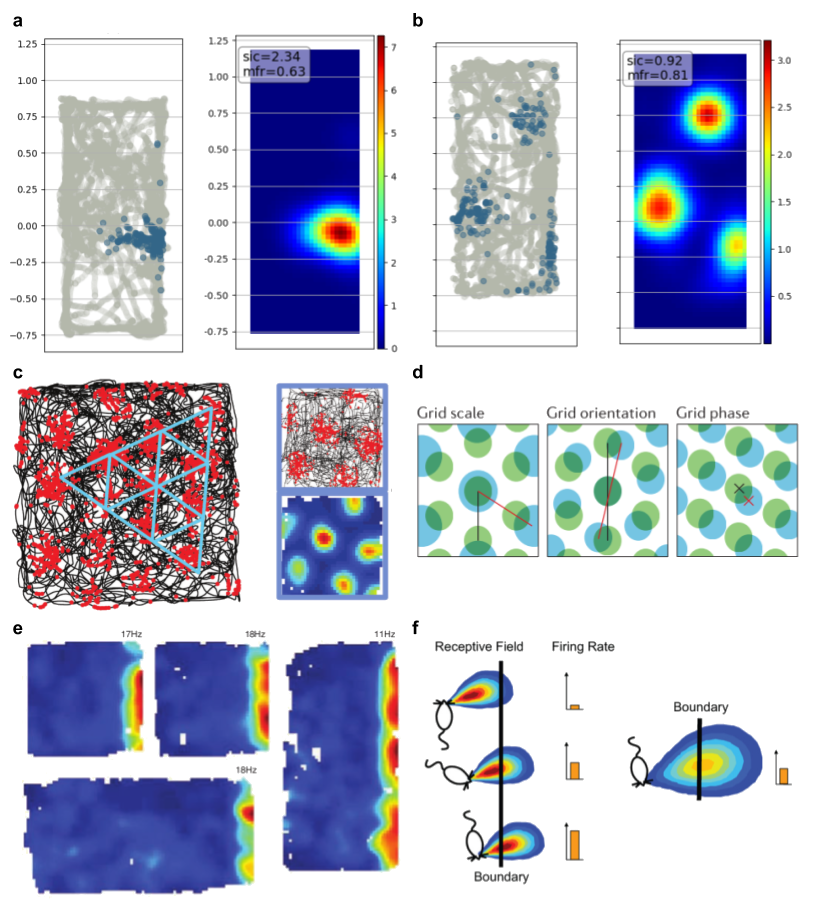
\includegraphics[width=150mm]{figures/F1_place_cells.png}}
\caption[Place and grid cells]{
Place, grid and border cells. \textbf{(a)} Firing rate map of an example hippocampal neuron that is active at a certain location in the rectangular environment - a “place” field. \textbf{(b)} another example neuron that has multiple place fields of different size (examples from the data used in the current study). \textbf{(c)} Firing rate map of an example mEC neuron that is active at certain locations of the environment, that form a hexagonal grid pattern (left). Place preference autocorrelograms reveal hexagonal structure (Adapted with permission from \cite{Moser2015}) \textbf{(d)} Examples of pairs of grid cells having different scale, orientation and phase (adapted with permission from \cite{Moser2014}). \textbf{(e)} Firing rate maps of an example neuron that is active near the right border of the environment, invariant of the environment type (adapted with permission from \cite{Solstad2008}) \textbf{(f)} schematic of the receptive field of an example neuron that is selective for a particular direction and distance to the environmental boundary (\cite{Lever2009}).
}
\label{fig:F1_place_cells}
\end{figure}


\subsection{Grid cells}

In addition to the discovery of the place cells, a few decades after, another important type of the place-selective cells were found in the brain’s entorhinal cortices. Particularly, in the layer II of the Medial Entorhinal Cortex (mEC) neurons, forming discrete regularly spaced firing fields were identified (\cite{Hafting2005}). Surprisingly, the firing fields of those neurons were organized in a grid of tessellating triangles evenly covering the corresponding space (Figure 1c). A simple autocorrelogram analysis revealed the rigid hexagonal structure (Figure 1c right). Key features of the newly discovered cells were, first - their different spacing between individual fields and phase shift relative to each other, with the increasing scale from dorsal to ventral mEC, and second - their anchoring to the boundaries, persistence between environments and independence on visual or olfactory landmarks. These facts suggest this type of cells is primarily based on self-motion and plays a main role in path integration, mixing idiothetic vestibular and proprioceptive signals.
Anatomically, mEC has a direct input to the Hippocampus. This led to the assumption that grid cells, sharing common peak and different spacing, might be a good basis to form place cells, taking grid cell inputs as a linear combination (\cite{OKeefe2005}). However, experimental evidence, based on studies on developing animals, shows that mechanisms are more sophisticated, as there is a delayed maturation of the grid fields relative to place cells. An alternative assumption, that place cells can be formed as a combination of the grid and other cell-type inputs - like border cells (see below), which are ready at the early stages of the development, looked to be more consistent. As suggested (\cite{Savelli2008}), specific place cells may arise as neurons integrating inputs from grid cells that provide proprioceptive-based distance information, and border cells that provide position relative to external boundaries. This putative idiothetic place cells will be named “boundary-driven” or “boundary-vector” cells later in the text.


\subsection{Head direction system}

One of the key components for successful navigation is maintenance of the proper allocentric orientation. Even before grid cells, neurons, which firing rates depend on the animal’s head orientation were found - originally in postsubiculum (\cite{Taube2007}), and later in other nearby areas (mEC, AdN etc.). Besides their primary feature of keeping the absolute directional preference, the “head-direction” cells were shown to maintain their relative directional preferences between each other; however, each cell by itself has no particular preference in absolute world coordinates - its directional preference can change between different environments. Importantly, in absence of light, head direction cells are able to integrate angular velocity of the head and maintain original directional preference, although for the cost of accumulation of directional error.

The presence of head direction cells is a necessary part to perform successful path integration, especially when light or external allocentric sensory cues are not present. The interaction of grid cells, providing distance estimation and a metric for space based on idiothetic inputs, and head direction cells supplying absolute orientation define the basis for position estimation based on path integration, which  is discussed more in one of the next sections of this chapter.


\subsection{Border and BVC cells}

While grid cells and head direction cells provide distance and orientation estimation, respectively, actual position should be estimated in relation to a certain point in space - usually relative to a physical boundary. Further research of the cell functions in the mEC lead to a discovery of the neurons representing geometric boundaries (\cite{Solstad2008}), and cells active at a particular distance to a certain boundary. These “border” and “boundary” cells are active when an animal is located near a certain physical boundary; their firing is independent of affine transformations (Figure 1e). A border cell, or more generally, a putative boundary vector cell (\cite{Barry2006}, \cite{Lever2009}), is another type of the neuronal encoding found in the mEC, that is involved in spatial representation. In a series of recordings these cells demonstrated preference to fire at a certain distance and direction to a particular object (Figure 1f) or, as a special case, to a certain boundary.

Border and boundary-vector cells (BVCs) may play an important role in updating positional signals of grid cells, as the latter tend to drift in open spaces. If the animal hits the boundary, any accumulated error in the grid cell positioning can be “reset” and appropriately corrected (\cite{Hardcastle2015}). Taken together, by defining the perimeter and stable physical objects relative to this perimeter inside, border and object-vector cells may represent an independent reference frame that can be used later by place cells to form correct space representations in the hippocampus.


\subsection{Landmark and object vector cells}

Besides environmental boundaries, stable visual landmarks can be used for building navigational strategies. In the visual sensory domain, cells, selective for certain spatial landmarks were discovered in the LEC (mEC) (\cite{Deshmukh2011}; \cite{Kinkhabwala2020}), and later in the CA1 and CA3 (\cite{Deshmukh2013}). These different selectivity types are ranging from an increase of neuron’s activity when passing a certain visual cue on the linear tracks (\cite{Kinkhabwala2020}), up to forming a stable firing field relative to a landmark at a certain distance and orientation. This discovery was further developed to a concept of general object vector cells found in the mEC, pointing to an idea that vector coding is a dominant form of position coding the entorhinal system (\cite{Hooydal2019}).


\subsection{Anatomy of the hippocampal-entorhinal system}

To establish meaningful conclusions about the mechanisms of the spatial navigation system, it’s important to explore the basic anatomical and functional connectivity of the underlying brain regions. Below we provide an essential extraction from the review of the anatomy of the hippocampal formation and the entorhinal cortex regions as the key areas involved in navigation, based on the rodent brain.

First we focus on the sagittal view of the rat’s right hemisphere, a horizontal brain slice in the middle of the hippocampal formation (Figure 2a). The hippocampal formation is presented by the key areas CA1, CA2 and CA3, as well as the DG and Subiculum. Darker areas show a density of pyramidal cell types (stratum pyramidale), where most of the place selective hippocampal neurons are found; lighter areas mostly contain dendrites and interneurons. The Parahippocampal region is represented by LEC, mEC, PrS and PaS areas. These regions contain the aforementioned grid cells and boundary-vector cells, as well as neurons selective to absolute orientations.

Pyramidal cells are excitatory cells that use Glutamate as a neurotransmitter. Different types of interneurons are all GABAergic (inhibitory), having their cell bodies distributed within all layers of the hippocampal formation (stratum radiatum, pyramidale, lacunosum-moleculare, oriens). Importantly, the activity of pyramidal cells are modulated by both external (e.g. mEC neurons) and internal (like CA3 principal cells and local inhibitory interneurons) inputs. One can distinguish principal cells and interneurons from electrophysiology. Principal cells have larger action potentials, have in average lower mean firing rate, and show noticeable bursty behavior.

The main cortical input to the hippocampus is the input from the entorhinal cortex that goes via the perforant pathway. Essentially this input conveys pre-processed information from higher-order sensory and association areas. In particular, most of the neurons of the layer 2 of the EC project to the DG and CA3, at the same time neurons in the layer 3 find their targets in the CA1 and Subiculum. CA1 and Subiculum provide feedback connections to the EC layer 5. There is a complex topography: all entorhinal layers are reciprocally connected (Figure 2b). In addition, there is also a mEC projection to the contralateral hippocampus with the same topography, although of a smaller density.

In essence, in the context of formation of place cells, the presented hippocampal-entorhinal connectivity allows for integration of the different mEC / LEC types of inputs with local CA3 inputs at the level of the CA1 pyramidal cells. This forms an anatomical basis for the assumption of the integration of grid, or boundary-vector cells, coming from the EC, with sensory driven cells - like visual landmark cells for the transient formation of the stable spatial representation in the form of place cells in the CA1 region.

\begin{figure}
\captionsetup{format=plain}
\makebox[\textwidth]{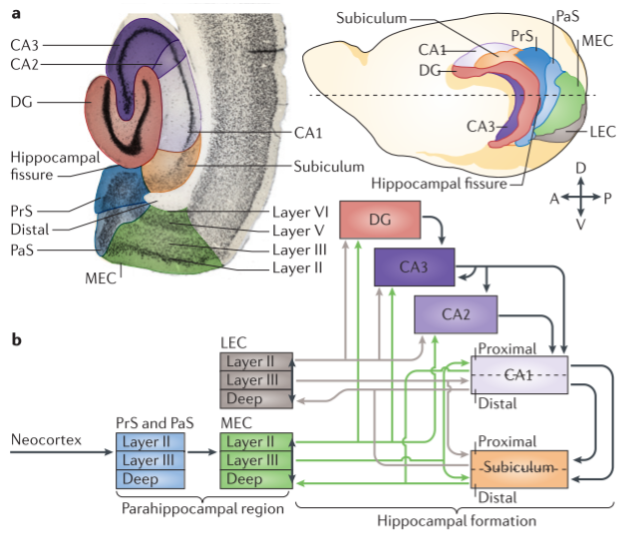
\includegraphics[width=150mm]{figures/F2_HPC_anatomy.png}}
\caption[Hippocampal-entorhinal Anatomy]{
(a) A slice of the right hemisphere of the rat brain (left). The focus is made on hippocampal and entorhinal regions. The same regions are shown located inside the rat brain (right). (b) Schematic of the connections within and between hippocampus and entorhinal cortex (adapted with permission from \cite{Moser2014})
}
\label{fig:F2_HPC_anatomy}
\end{figure}


\subsection{Sequence coding and theta phase precession in hippocampal cells}

As was established in the end of 1960x, hippocampal local field potential (LFP) activity provides oscillations of different modes and frequencies (\cite{Vanderwolf1969}). There are two main regimes - a prominent oscillation in a range between 7 to 12 Hz named Theta oscillation, and other irregular activity with broader spectrum of frequencies, including Gamma periods, Sharp-Wave Ripples (SWRs) and others. In rodents, theta oscillation highly correlates with animal actions and movements - running, jumping, grooming (\cite{OKeefe1993}). Here we focus on the theta regime and the corresponding animal behaviors, as they have an intrinsic connection with hippocampal cells.

Looking more detailed at these hippocampal place cells, an outstanding feature of the place cells behavior is their ability to lock their activity to a certain phase of the theta oscillation, when an animal runs through a place field (Figure 3a). While crossing a place field in one-dimensional or two-dimensional environment, place cell discharges in spiking bursts at progressively earlier phases of the theta rhythm, from spiking at peak of theta oscillation when entering a place field, having the highest firing rate (middle of the place field) on the trough to later spikes when exiting a place field on the ascending phase of theta oscillation (\cite{Jensen1996}, \cite{Skaggs1996}, \cite{Tsodyks1996}, \cite{Dragoi2006}).

This mechanism of spiking bursts within regular time windows is important for linking related path segments using the spike-timing dependent plasticity (\cite{Dan2004}). Importantly, the same mechanism might be useful for successful integration of the coherently incoming feature-extracted information of different modality, like the positional information relative to the spatial boundaries (boundary vector cells) and positional information relative to visual cues or landmarks (visual object vector cells), forming a unique spatial representation. More generally, the same mechanism, when used to integrate non-positional information like odors, sounds, or reward expectations, could be the basis of forming time-invariant memories, or episodes (\cite{Buzsaki2018}).


\begin{figure}
\captionsetup{format=plain}
\makebox[\textwidth]{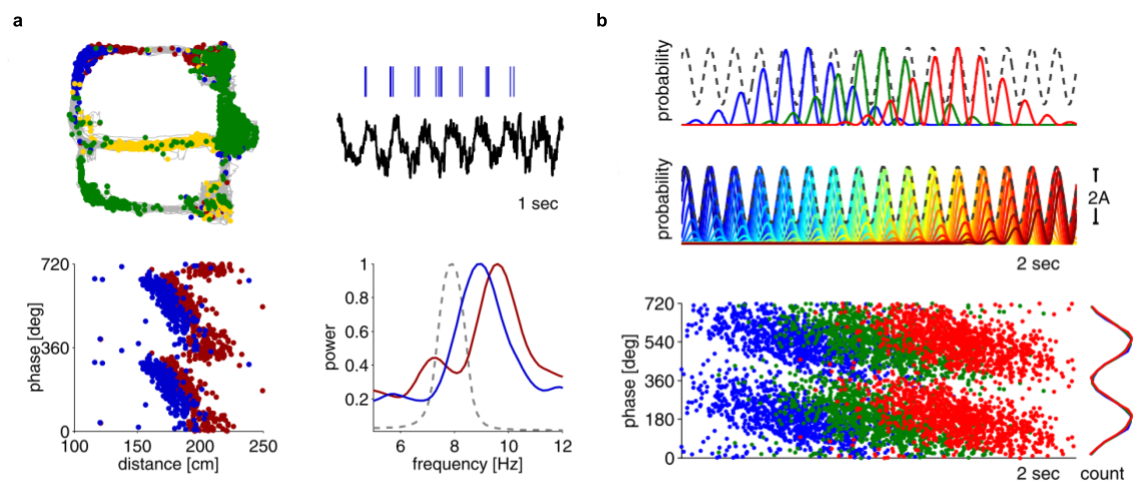
\includegraphics[width=150mm]{figures/F3_phase_precession.png}}
\caption[Theta phase precession]{
(a) A phenomena of the spiking precession of hippocampal neurons relative to the internal LFP theta oscillation. A neuron spiking is chunked by the oscillation and appears earlier in phase as a rat goes through a place field. (b) Sequences of memories and their interference (top), spiking phase relative to the theta oscillation (adapted from \cite{Geisler2010}; permission not required).
}
\label{fig:F3_phase_precession}
\end{figure}



\subsection{Formation of place fields}

Grid, border and head direction cells in the mEC together form one independent representation of space, stable between environments. The reciprocal representation is constructed by hippocampal place cells, that often fully remap between different environments, forming an unique representation of a particular space. These two spatial representations are complementary: one expresses the metric of a space independent of the specific landmarks or action-defined context, another is sensitive to the unique experiences in that space, location of objects or landmarks, building a number of context-dependent orthogonal representations.

The experimental evidence of the increased density of hippocampal place fields near corners and boundaries compared to the center of the environment (\cite{Wiener2737}) leads to a suggestion of a high level of a direct contribution of the border cells to the formation of place fields. Another fact supporting this hypothesis, is that border cells in the mEC are available in the early development - as do place cells when an animal explores an environment on the first day. This leads to an assumption that border cells might have a larger influence on place cells in youth, with the increasing role of grid and other types of mEC cells in adulthood.

Importantly, there is a bidirectional connectivity between hippocampus and entorhinal cortex (see - hippocampal anatomy), the latter receiving feedback from the hippocampus that may be essential for the formation or maintenance of entorhinal spatial maps. This is supported by the experimental evidence that the inactivation of the hippocampal inputs leads to the loss of hexagonal firing pattern of grid cells (\cite{Bonnevie2013}). These facts might be crucial for the explanation of the effects of place cell behavior presented in the results section.

To build experience-dependent representations, place cells need to interact with a variety of entorhinal cell assemblies, carrying distinct types of information. The efficiency and domination of different input types depends on intrinsic properties, like synaptic plasticity, but also on interaction with the environment - animal running speed, behavior, or environmental changes (\cite{Igarashi2014}). It is not yet clear if some of the input types dominate the other, and how place cells recruit synaptic inputs of a certain type to build stable spatial fields. In this work I try to address these questions and to demonstrate that in some particular conditions these inputs of allocentric and idiothetic nature are mixed, and try to further explore the dynamic balance between them.


\subsection{General questions}

The mechanisms that implement spatial navigation in the hippocampal-entorhinal system are not fully described and understood. Among open questions are the mystery behind the formation of the grid patterns, the phenomenon of theta phase precession, the role of gamma oscillations in memory consolidation, how and where the path integration is implemented and many others. Here in this study I focus on the phenomena of place cells in the CA1 region of the hippocampus, especially on the integration of the idiothetic, or precisely boundary-driven information and the visual, landmark driven information into a reliable space representation. The interaction between these allothetic and idiothetic inputs at the level of their postsynaptic influence, especially when they are in conflict, is not yet fully understood. Ultimately, these interactions may reveal, if described in detail, the more general mechanisms of episodic memory formation within the hippocampus which could be extended from navigation to a broad range of behavioral applications, including general action planning and abstract thinking.


%\section{The role of visual landmarks and physical boundaries in spatial navigation}
\section[The role of visual landmarks and physical boundaries in spatial navigation]{The role of visual landmarks and physical boundaries in spatial navigation%
              \sectionmark{The role of visual landmarks and physical boundaries}}
\sectionmark{The role of visual landmarks and physical boundaries}

\label{sec:role_of_landmarks}


\subsection{What is a place?}

A place in physical space can be uniquely defined by a set of reference points and landmarks, similar to it’s representative location on an allocentric map. Place is usually considered invariant of time and independent of the way how a subject gets there. This invariance connects the definition of place to the broader definition of semantic memory - invariant stable description of living things, facts or other knowledge (\cite{Buzsaki2013}). Repeated exploration of the environment allows subjects to revisit the same location multiple times, gradually building its representation from recurrent similar episodes - by linking together different (in time) episodes that share the same set of features, landmarks and relations between them.

High-level feature extraction is necessary to build a coherent representation of space, mainly because early sensory systems predominantly encode very simple stimulus modalities with very localized receptive fields. These would not be enough to build similar episodes sharing the same set of features, in case, for example, an animal reached the same location from opposite sides - and  experienced some different visual flow, experienced a set of new sounds, or made a different number of steps walking from the other boundary. Higher brain areas like hippocampus or cortical areas, involved in both memory and navigation, need to operate with higher order features like boundaries, objects of different shape, visual and olfactory landmarks, in order to be able to combine them as a set of similar combinations of sensory features (episodes) to an invariant representation of a particular location. As was shown in the first section, these operations of high-order feature selectivity might mainly reside in the mEC/LEC, being mostly implemented by boundary, object, and landmark vector cells. As anatomically hippocampus receives its major input from the entorhinal cortices, its role in navigation, shown by place cells, might be to orchestrate these incoming navigational information elements to either build and store a new place memory - a unique constellation of features, representing new location, or to update already existing place memory, if this set of features is similar to the already experienced number of stable objects, shapes and cues at a certain distance.

While external sensory information about distinctive and stable environmental features is necessary to build a stable allocentric map, the internal idiothetic information is required to both support this initial formation, as well as to maintain the constructed representation when the external information is partially or completely not available - for example, in total darkness. Our brains are able to maintain the allocentric position and navigate in space without external inputs, for the price of some error accumulation (\cite{Etienne1988}; \cite{Etienne2004a}). This is an indispensable function of the internal navigation system, essential for successful survival and evolution. The implementation of that feature requires an integration of the information coming from the internal idiothetic system into the circuits, encoding spatial maps. This aspect of establishing, recalling and maintaining the spatial map in absence of sensory inputs are discussed below in this chapter.


\subsection{Landmark and boundary vectors as reference frames to establish spatial map}

Overall, to build a spatial map one needs to define a set of related places (in the brain - place fields) having a certain position within a particular spatial reference frame. A reference frame can be defined as an independent coordinate system, having a definite distance and orientation to one or several reference points. Following this classical definition both environmental boundaries and a set of visually defined landmarks can serve as two independent reference frames, if they don’t change their relational stability between reference points within itself. When it is the case, the aforementioned landmark vector cells and boundary vector cells (\cite{Deshmukh2011}; \cite{Hooydal2019}) can be used to represent two reference frames of different modality in the brain.

While exploring the new environment, these inputs from the boundary vector cells and landmark vector cells (as well as other sensory modalities - olfactory, auditory etc.) are integrated to form coherent stable points, or recurrent episodes, which taken altogether, can be used to form a consistent allocentric representation of the surrounding environment. While moving from one place to another, animal revisits the places, formed of the similar set of environmental features, and reactivates the very similar sensory inputs which, with the help of some pattern completion mechanisms, updates and sharpens the CA1 ensemble representation of a particular physical location - place field in the hippocampal memory system. This movement from one place to another builds a trajectory - a set of connected physical places as an animal path, as well as the set of activated and connected places fields as a virtual path in the brain (\cite{Buzsaki2013}).


\subsection{Mechanisms of path integration to support navigation stability}


To maintain the navigational stability when allocentric cues are removed, the internal navigation system, including place cells, continues to track location using self-motion. Path integration is essentially a computation transforming a change in motion into a change in position. Having a current position estimate, one can derive a new allocentric position by tracking angular movements and distance travelled. Whether this system is based on continuous integration of angular or linear velocities, or on addition of a distance travelled vector to the current estimate - it is based on cues derived from the inputs from the self-motion systems (\cite{Etienne2004a}). These cues include vestibular, proprioceptive cues or motor efference copy (step counting). Additionally, a change in airflow (e.g. sensed by whiskers) or vibration from textures while moving can support speed calculation and resulting translation detection (\cite{Savelli2019}).

How can the path integration system be implemented in the brain circuits? While both distance and angular movement signals coming from grid and head direction cells tend to drift in open spaces without correction by particular cues or landmarks (\cite{Barry2007}), they are still the great candidates to support the path integration system. Boundary cells, or the tactile sensory inputs in the environmental corners, can episodically reset the grid and head direction inputs bringing the path integration system up to date with the environment position and orientation (\cite{Barry2007}; \cite{Cheung2012}). This leads to an assumption that path integration is mainly implemented in the cerebral cortex in a form of an attractor-network (\cite{Knierim2012}; \cite{McNaughton2006}), supported by the fact that the hippocampal upstream regions have all necessary components.

Another reported alternative is that the path integration computations are performed in lower regions, subcortically, reflecting the organization of the head direction system (\cite{Savelli2019}). As thalamic or other subcortical regions already receive vestibular and motor signals, they are able to compute and integrate angular and translational velocity signals, implementing basic path integration. The anatomical structure of the head direction system, for instance, with head direction cells found in anterior dorsal thalamic nucleus (\cite{Taube1995}) is another evidence to support this alternative.


\subsection{Impact on place cells}

Navigation at the level of hippocampal formation with its place cells are the main focus of this study. There is evidence showing that place cells follow visual cues (\cite{Muller1987}; \cite{Deshmukh2013}; \cite{Aronov2014}), suggesting that they receive incoming allocentric information. There is also a large evidence showing that place cells are able to maintain their place preference in case the sensory inputs are removed (\cite{Gothard2001}; \cite{Quirk1990}). In conflicting situations, as was shown in virtual reality (VR) studies (\cite{Gothard2001}; \cite{Haas2019}), cells are able to switch from one to another reference frame in their selective firing, suggesting integration of allothetic and idiothetic inputs. As described in the previous sections of this chapter, initial sensory processing and feature extraction, as well as path integration happens mainly outside the hippocampus. Taken together - how exactly these different pathways are integrated within the hippocampal neural circuits? This question is still not well understood. Below I review a few model studies exploring potential mechanisms of this integration (see modelling section).


\section{Research on interaction of allothetic and idiothetic inputs}
\label{sec:interaction_allo_idio}

One of the first seminal research studies of the effect of the allothetic environmental changes on place cells was done in 1987. Muller and Kubie (\cite{Muller1987}) showed that the rotation of a visual cue card, but not its width or shape, produces rotation of the place fields in a cylindrical arena. Removing the card led to a randomized angular representation of the arena. These recordings demonstrated direct dependence of the place field orientation on the visual information, implicating that cells in the hippocampus are modulated by allothetic visual inputs.

Getting more detailed, several years later, it was shown that objects located near the center of the arena could not control the orientation of the place fields in the environment, but do that with a help of a cue card on the wall (\cite{Cressant1997}). Same objects, placed near the walls enable control over the fields orientation, indicating that involvement of the head direction system, that potentially resets angular orientation relative to the unique objects, located close to the environmental borders.

The question of interaction of allocentric and idiothetic representations got more specificity in later studies by Bures and Zahalka (\cite{Bures1998}), where they experimentally trained animals to avoid foot shocks using either room landmarks or using idiothetically defined area on the floor. The ability of rats to avoid shock locations defined in both reference frames showed credible independence of the allocentric and idiothetic mechanisms, encoding two reference frames. However, a question of how these two systems are intermixed remained unclear.

Gothard and McNaughton proposed that place cells, mainly driven by internal “path integrator” - accumulated internally-driven translational information about a movement in space together with head direction cells - form a preconfigured network of a two-dimensional space. This network is updated by the visually-specific landmark information using associative learning (\cite{Mcnaughton1996}). They performed a series of experiments with rats on the linear track where two separate reference frames were used by a rat to track self position. By gradually moving these reference frames (a reward site and a starting box), they found both cells fired at fixed distances from the origin and cells fired at proximity to the destination. The same neuron was able to shift its spatial preference from being aligned to the origin to an alignment to the destination. They postulate that when mismatches between the visual and the idiothetic information occur, path integration and sensory cues competitively interact to affect place field preference (\cite{Gothard1996}). Their further recordings in light and dark conditions, showing that the box-referenced cells tend to keep their firing preference longer even without light, supported that idea. Ultimately, based on their moving-box-reward experimental data they suggest that interaction between internal dynamics and path integration and external sensory cues happens before both CA1 and CA3 areas, possibly in the entorhinal cortex or subiculum.

However the question of exact mechanism of position computation based on actual or path integrated information remained unclear. A new set of tools including virtual reality was introduced to continue the research of dynamics and circuitry implementing allocentric- and idiothetic- based navigation.


\begin{figure}
\captionsetup{format=plain}
\makebox[\textwidth]{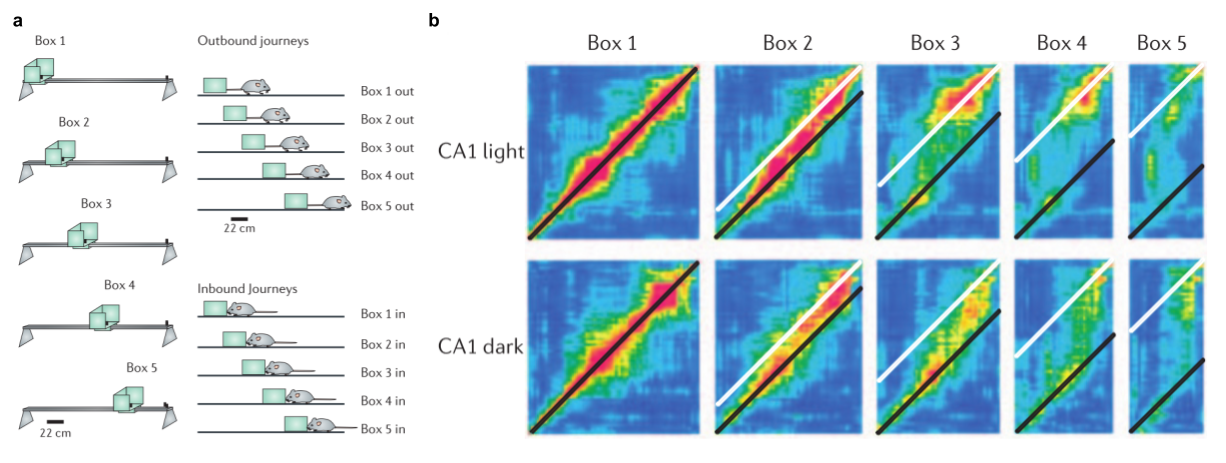
\includegraphics[width=150mm]{figures/F4_moving_box.png}}
\caption[Moving shelter as a reference frame]{
(a) A schematic of the experiment with a moving box. A starting box together with a reward location at the end of the track act as two independent reference frames. By gradually moving the box one can investigate the change of the spatial encoding relative to either of the frames. (b) The resulting place cell firing in light and dark establish gradual shift in encoding position (adapted with permission from \cite{McNaughton2006})
}
\label{fig:F4_moving_box}
\end{figure}


%\section{Optimal combination of environmental cues and path integration during navigation}
\section[Optimal combination of environmental cues and path integration during navigation]{Optimal combination of environmental cues and path integration during navigation%
              \sectionmark{Optimal combination of environmental cues}}
\sectionmark{Optimal combination of environmental cues}
\label{sec:optimal_comb_for_spat_nav}

How algorithmically do the allocentric and idiothetic inputs merge at the level of the hippocampal place cells? When the brain needs to integrate information of different sensory modalities it often uses “optimal” combination - a weighted sum of the inputs with weights proportional to their reliability. This has been established in many behavioral and theoretical studies for humans (\cite{Ernst2002}; \cite{Alais2004}; \cite{Knill2003}; \cite{Hillis2004}) for combinations of different sensory modalities (visual / auditory, visual / haptic, stereo / texture, environmental geometry / path integration etc.). The optimal coding theory is also applicable for spatial navigation. In a series of behavioral studies position estimation based on Bayesian decoding was established and predicted. In particular, optimal cue integration is demonstrated in ants (\cite{Wystrach2015}), rats  (\cite{Shettleworth2005}) or humans (\cite{Zhao2015}; \cite{Chen2017}; \cite{Sjolund2018}). However, while real-world navigation normally implies redundant integration of external, allocentric, cues and internal, idiothetic or path-integration based position estimations, is that combination always optimal?


\begin{figure}
\captionsetup{format=plain}
\makebox[\textwidth]{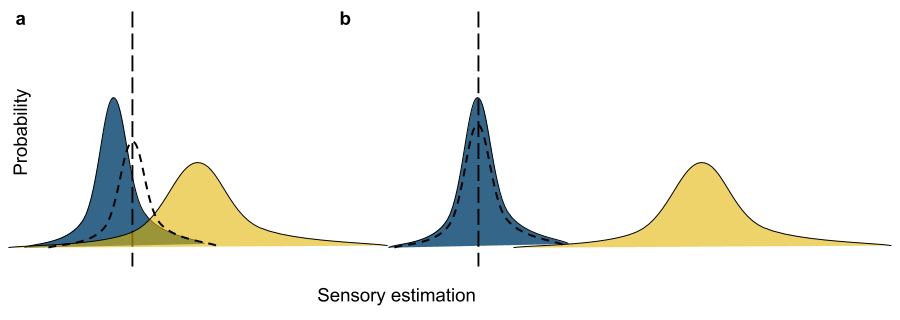
\includegraphics[width=150mm]{figures/F5_larger_smaller_conflicts.png}}
\caption[Sensory conflicts of different size]{
Sensory integration at larger and smaller conflicts. (a) In a situation of a small conflict between estimations it is beneficial to use optimal coding - a weighted combination of the estimation with weights proportional to their reliability (variance). Also named Bayesian decoding, or maximum likelihood estimation (MLE). (b) In a situation of a large conflict between estimations a strategy of abandonment of a less reliable information source will have higher chances to end with a better precision.
}
\label{fig:F5_larger_smaller_conflicts}
\end{figure}


Intuitively, when the conflict between two given estimations is small, weighted integration and resulting averaging makes sense. Especially if performed in an optimal, Bayesian way, it allows for a maximization of the precision of the resulting estimate, attributing a conflict to a sensory noise (Figure 5a). On the other hand, situations of a large conflict might be caused by misidentification of an object identity, incorrect memory retrieval or in general - failure in estimation based on a particular sensory source. In that case Bayesian integration might lead to large errors relative to both information sources, while full abandonment of one, ideally less reliable, source of estimate might be a logical choice (Figure 5b). This abandonment of one source, or cue, in favor of the other has been demonstrated in animal and human navigation studies. For instance, when humans were presented with a large > 115 degrees conflict between landmark and path integration cues they prefered path integration (\cite{ZHAO201596}). Rats in large spatial conflicts also prefer to rely on path integration in favor of a single landmark (\cite{Shettleworth2005}).

While the ability of a brain to implement optimal coding is well known, however it has not been thoroughly explored at the physiological level. Different potential schemes, including gain field theory, convolutional encoding, doubly distributional population coding were introduced (see review in \cite{Pouget2003}), however it is still not clear which scheme is used by the neurons or whether neurons actually encode continuous distributions at the population level. In this work, we address this question and make an attempt to show on the cellular level how these mechanisms of estimation integration at small conflicts and estimation abandonment at large conflicts could be implemented by a population of hippocampal neurons. We hypothesize that attractor dynamics in the hippocampal circuits might implement nearly-optimal coding for spatial and potentially non-spatial estimations, predicted earlier in other sensory systems (\cite{Jeffery2016}) and how the abandonment of less reliable estimation could be implemented at the level of a single neuron.


\section{Modelling multisensory integration at the level of place cells}
\label{sec:modelling}

“…Each place cell receives two different inputs, one conveying information about a large number of environmental stimuli or events, and the other from a navigational system which calculates where an animal is in an environment independently of the stimuli impinging on it at that moment. The input from the navigational system gates the environmental input, allowing only those stimuli occurring when the animal is in a particular place to excite a particular cell…” - an original sentence by O’Keefe led to a general proposal that the place cells might integrate idiothetic information coming from the different cell groups from the entorhinal cortex with some other sensory information.

Initially, a discovery of grid cells led to a model proposed by Solstad and Einevoll, which assumed formation of place cells via linear summation of weighted inputs from the grid cells (\cite{Solstad2006}). It was suggested that irregularly spaced place fields can appear as a result of summing inputs from entorhinal cells with different spacing and orientation, and relatively similar grid phases. However, this model was free from complex network interactions and required having place cells integrating grid cell inputs with overlapping vertices. This issue was fixed later by demonstrating that adding fast hebbian plasticity may result in the careful selection of appropriate inputs, without the need for specific network wiring (\cite{Savelli2010}).

The discovery of border cells and boundary vector cells led to another approach, assuming that environmental boundaries can serve as determinants of the hippocampal place fields. The boundary vector cell model (\cite{Barry2006}) describes place fields emerging from a combination of cells active at a certain direction and orientation relative to the environmental boundaries.

However, both of these approaches were focused on feed-forward type of information transfer, uni-directional communication between cortex and hippocampus. Recently, a novel approach connecting feed-forward information flow from the entorhinal layers to the hippocampus with feedback flow to the entorhinal areas, was proposed (\cite{Li2020}). It is a model that assumes continuous interaction between grid and place cells, with plasticity mechanisms enabling balance in control over place definition between vision and self-motion, allocentric and idiothetic inputs. In this model, self-motion is represented by multiple layers of grid cells that integrate angular and translational movement velocities (see grid cells). Visual input is modelled using a retina-like grid with Gabor filters, applied to the incoming stream of camera images. It is also assumed that it gets input from the head direction system such that the resulting visual information in particular location is independent from head orientation, similar to the non-grid cell in the LEC (see object-vector cells). Competitive organization of the network outputs establishes two different populations of place-selective cells - purely self-motion (or boundary) driven (motion place cells - MPCs), and purely visually driven (visual place cells - VPCs). These cells are assumed to be present in the CA3 regions of the hippocampus and together provide informative inputs to CA1 place cells. Having hebbian plasticity mechanisms and feedback connections back to the self-motion grid cells (MPCs), these latter CA1 cell are classified into 3 major groups - visually driven, self-motion or boundary driven and multisensory cells, that combine both of the allothetic and idiothetic inputs. These simulation results are very similar to the previously reported results (\cite{Haas2019}), as well as they highly correlate to the new electrophysiological data from the current study. Here I found very similar groups of neurons, having similar spatial firing properties (see Results). However, the disadvantage of the model is that it does not account for border-defined inputs which, as we also find in the neural data, might play an important role in correcting self-motion vectors and modulating the dynamics of the network as a whole.

Ultimately, considering models of the underlying neural dynamics, the current work is attempting to provide additional evidence for the modern loop-based approach to describe hippocampal-entorhinal networks implementing principles of spatial navigation. Based on the collected data, we hypothesize that hippocampal neurons implement a weighted combination of position estimation based on allocentric and idiothetic inputs in a nearly-optimal fashion. We show that the resulting position estimation influences self-motion based place representation, possibly via backprojections from the hippocampus to the entorhinal cortex. Overall this makes a step towards bringing evidence based on the neurophysiological data for the proposed model in situations, when place definitions are conflicting.


\section{Aim of the thesis}
\label{sec:aim_of_thesis}

For many years hippocampus has been identified as a brain structure, critical for spatial learning and navigation. The spatial domain extends beyond the traditional navigation in physical spaces - to many abstract spaces humans need to operate daily, not only to be partially efficient, but also to be successful in survival. Hippocampus, having specially tuned neurons - place fields - that rely on external sensory inputs and self-motion cues, mainly coming from the cortical areas, is able to implement high-level context-dependent representation of the environment. However it is still not known how exactly these different information flows interact to build a consistent and stable map of connected place fields.

Existing studies suggest that both proprioceptive and idiothetic types of information are continuously integrated to update the self-position (e.g. implementing “path integration”) while other stable sensory cues provide references to periodically update the allocentric position of self and correct it for the collected integration-related errors. It was shown that both allocentric and idiothetic types of information influence positional cell firing, however in most of the studies these inputs were firmly coupled. The use of virtual reality setups (\cite{Thurley2016}) made it possible to separate the influence of vision and proprioception for the price of not keeping natural conditions - the animal is usually head- or body-fixed (\cite{Holscher2005}; \cite{RavassardA.2013}; \cite{Jayakumar2018}), which introduces vestibular motor- and visual- conflicts, providing a bias for space encoding. Here we use the novel CAVE Virtual Reality system for freely-moving rodents (\cite{DelGrosso2018}) that allows to investigate the effect of visual- and positional- (vestibular) manipulation on the hippocampal space code while keeping natural behaving conditions.

Particularly, the current research is aimed at studying the impact of visual and vestibular (passive translation) manipulations on the hippocampal code using this novel freely-moving ratCAVE system. With the ability to manipulate the projected virtual environment and to unidirectionally move the physical arena depending on animal’s position, the following questions are addressed:

\begin{itemize}
  \item how would the stable visually-defined spatial reference frame impact the hippocampal place code when put in conflict with the moving space reference frame, defined by the physical boundaries
  \item would the passive physical move in space, locked to the physical boundaries and supported with vestibular inputs, differently impact the place code in contrast to the opposite situation when the move of the reference frame is just visual and not supported by the vestibular inputs - addressing the question of the role of vestibular information in coding the preference to one or another reference frame
	\item whether an instant mismatch between the visual and proprioceptive inputs (gain) would distort the hippocampal place map and at which threshold
	\item what types of the hippocampal place cells could be separated by their sensory and / or feedback inputs (visual, self-motion or boundary-driven or their combinations) and how strong is the path integration component
	\item whether a single instant conflict between information coming from the internal path integration system and the visual information can influence the current place code or lead to any remapping
\end{itemize}

In summary, we focus on the dynamic representation of space when the visual-cue-defined and physical-boundary-defined reference frames are in conflict. We confirm the dominance of one reference frame on the other on the level of place fields, when the information about one reference frame is absent (\cite{Gothard2001}). We show that the hippocampal cells form distinct categories by their input preference - surprisingly, not only that they are being driven either by visual / allocentric information or by the distance to the physical boundaries and path integration, but also by a specific combination of both. I found a large category of units integrating inputs from both allocentric and idiothetic pathways that are able to represent an average location between two reference frames, when they are in conflict. The use of virtual reality allowed me to demonstrate that these units become only path integrator driven when they lose their visual inputs. Based on the recorded information about these single cell theta phase-modulation, I propose a model how these units can integrate allocentric and idiothetic inputs to form this independent category of place representation.

Ultimately, the aim of the current work is to try to provide more support in linking the view over the hippocampus from the other side - to consider it not only as a spatial machine, but as a common generator of sequences of episodic memories (\cite{Buzsaki2013}), having place cells as examples of a particular recurrent episode - an integrated internal and external feature-processed sensory information at a particular moment of time, shaped by brain theta rhythms.


\chapter{Motivation \& Outline}
\label{ch:motivation_goal}

\section{Motivation}

The overarching purpose of this master's thesis is to outline the first steps taken towards building a generally reusable, automatic interpretation and hypothesis generation machine.

While many analyses, including those previously referenced, can successfully aid scientists in interpretation of data, each are developed with specific data sets, knowledge assemblies, or application scenarios in mind. Those that were developed using schemata that lacked the generalized multi-scale and multi-modal (schema-free) integration enabled by BEL could have potentially disregarded relevant and important knowledge. 

\section{Outline}

The first section of this thesis describes the PyBEL, the framework built to parse and manipulate BEL Script and resulting knowledge assemblies. The following section describes the development the Bio2BEL data integration framework and the beginning of a cross-scale data integration project similar to Pathway Commons. The final section describes the development of algorithms for analyzing the robustness of knowledge assemblies, preprocessing techniques, and ultimately, proposes a reusable, general, schema-free analytical technique that generates hypotheses with knowledge-driven analyses of data.


\chapter{PyBEL}
\label{ch:pybel}

\section{Survey of Current Technologies}

While there exist several software packages for \ac{BioPAX} and \ac{SBML}, the ecosystem of open-source software for \ac{BEL} is much more limited.

\subsection{OpenBEL Framework}

With its publication of the \ac{BEL} v1.0 specification as an open standard, the OpenBEL Consortium released the OpenBEL Framework \cite{openbelframework} ; a Java framework for parsing BEL v1.0 documents and its companion Cytoscape plugin \cite{openbelframeworkcytoscapeplugins} for network visualizations.

\subsection{bel.rb}
Ongoing development slowed \cite{openbelframeworkgraphs} as the focus of OpenBEL development shifted towards \verb|bel.rb| \cite{belrb}; a Ruby tool for parsing and transforming BEL v1.0 Script to \ac{RDF}. Additionally, there is only limited community support through GitHub and the proposed channel on Gitter.

Neither of the previously mentioned softwares provide explicitly documented support for this revision; and the aging codebase of the OpenBEL Framework and the generally low usage of Ruby in the bioinformatics community provide little incentive for updates. 

\section{Motivation}

There is an unmet need for publicly available, easily installable, stable, facile software that parses modern BEL and provides programmatic access to a data container that enables the resulting network to be extended, queried, manipulated, analyzed, and visualized. Furthermore, a converter between common data formats is needed to enable re-usability and interoperability between general and BEL-specific software for network analysis and visualization. This chapter presents PyBEL, a Python language software package designed to fulfill each of these needs.

\section{Software Architecture}

Development of the PyBEL software package adheres to a component-based software architecture. The schematic view in Figure 5 illustrates how data flows between components. components interact to build an integrated environment for working with networks encoded in BEL Script. 

\begin{figure}
\captionsetup{format=plain}
\makebox[\textwidth]{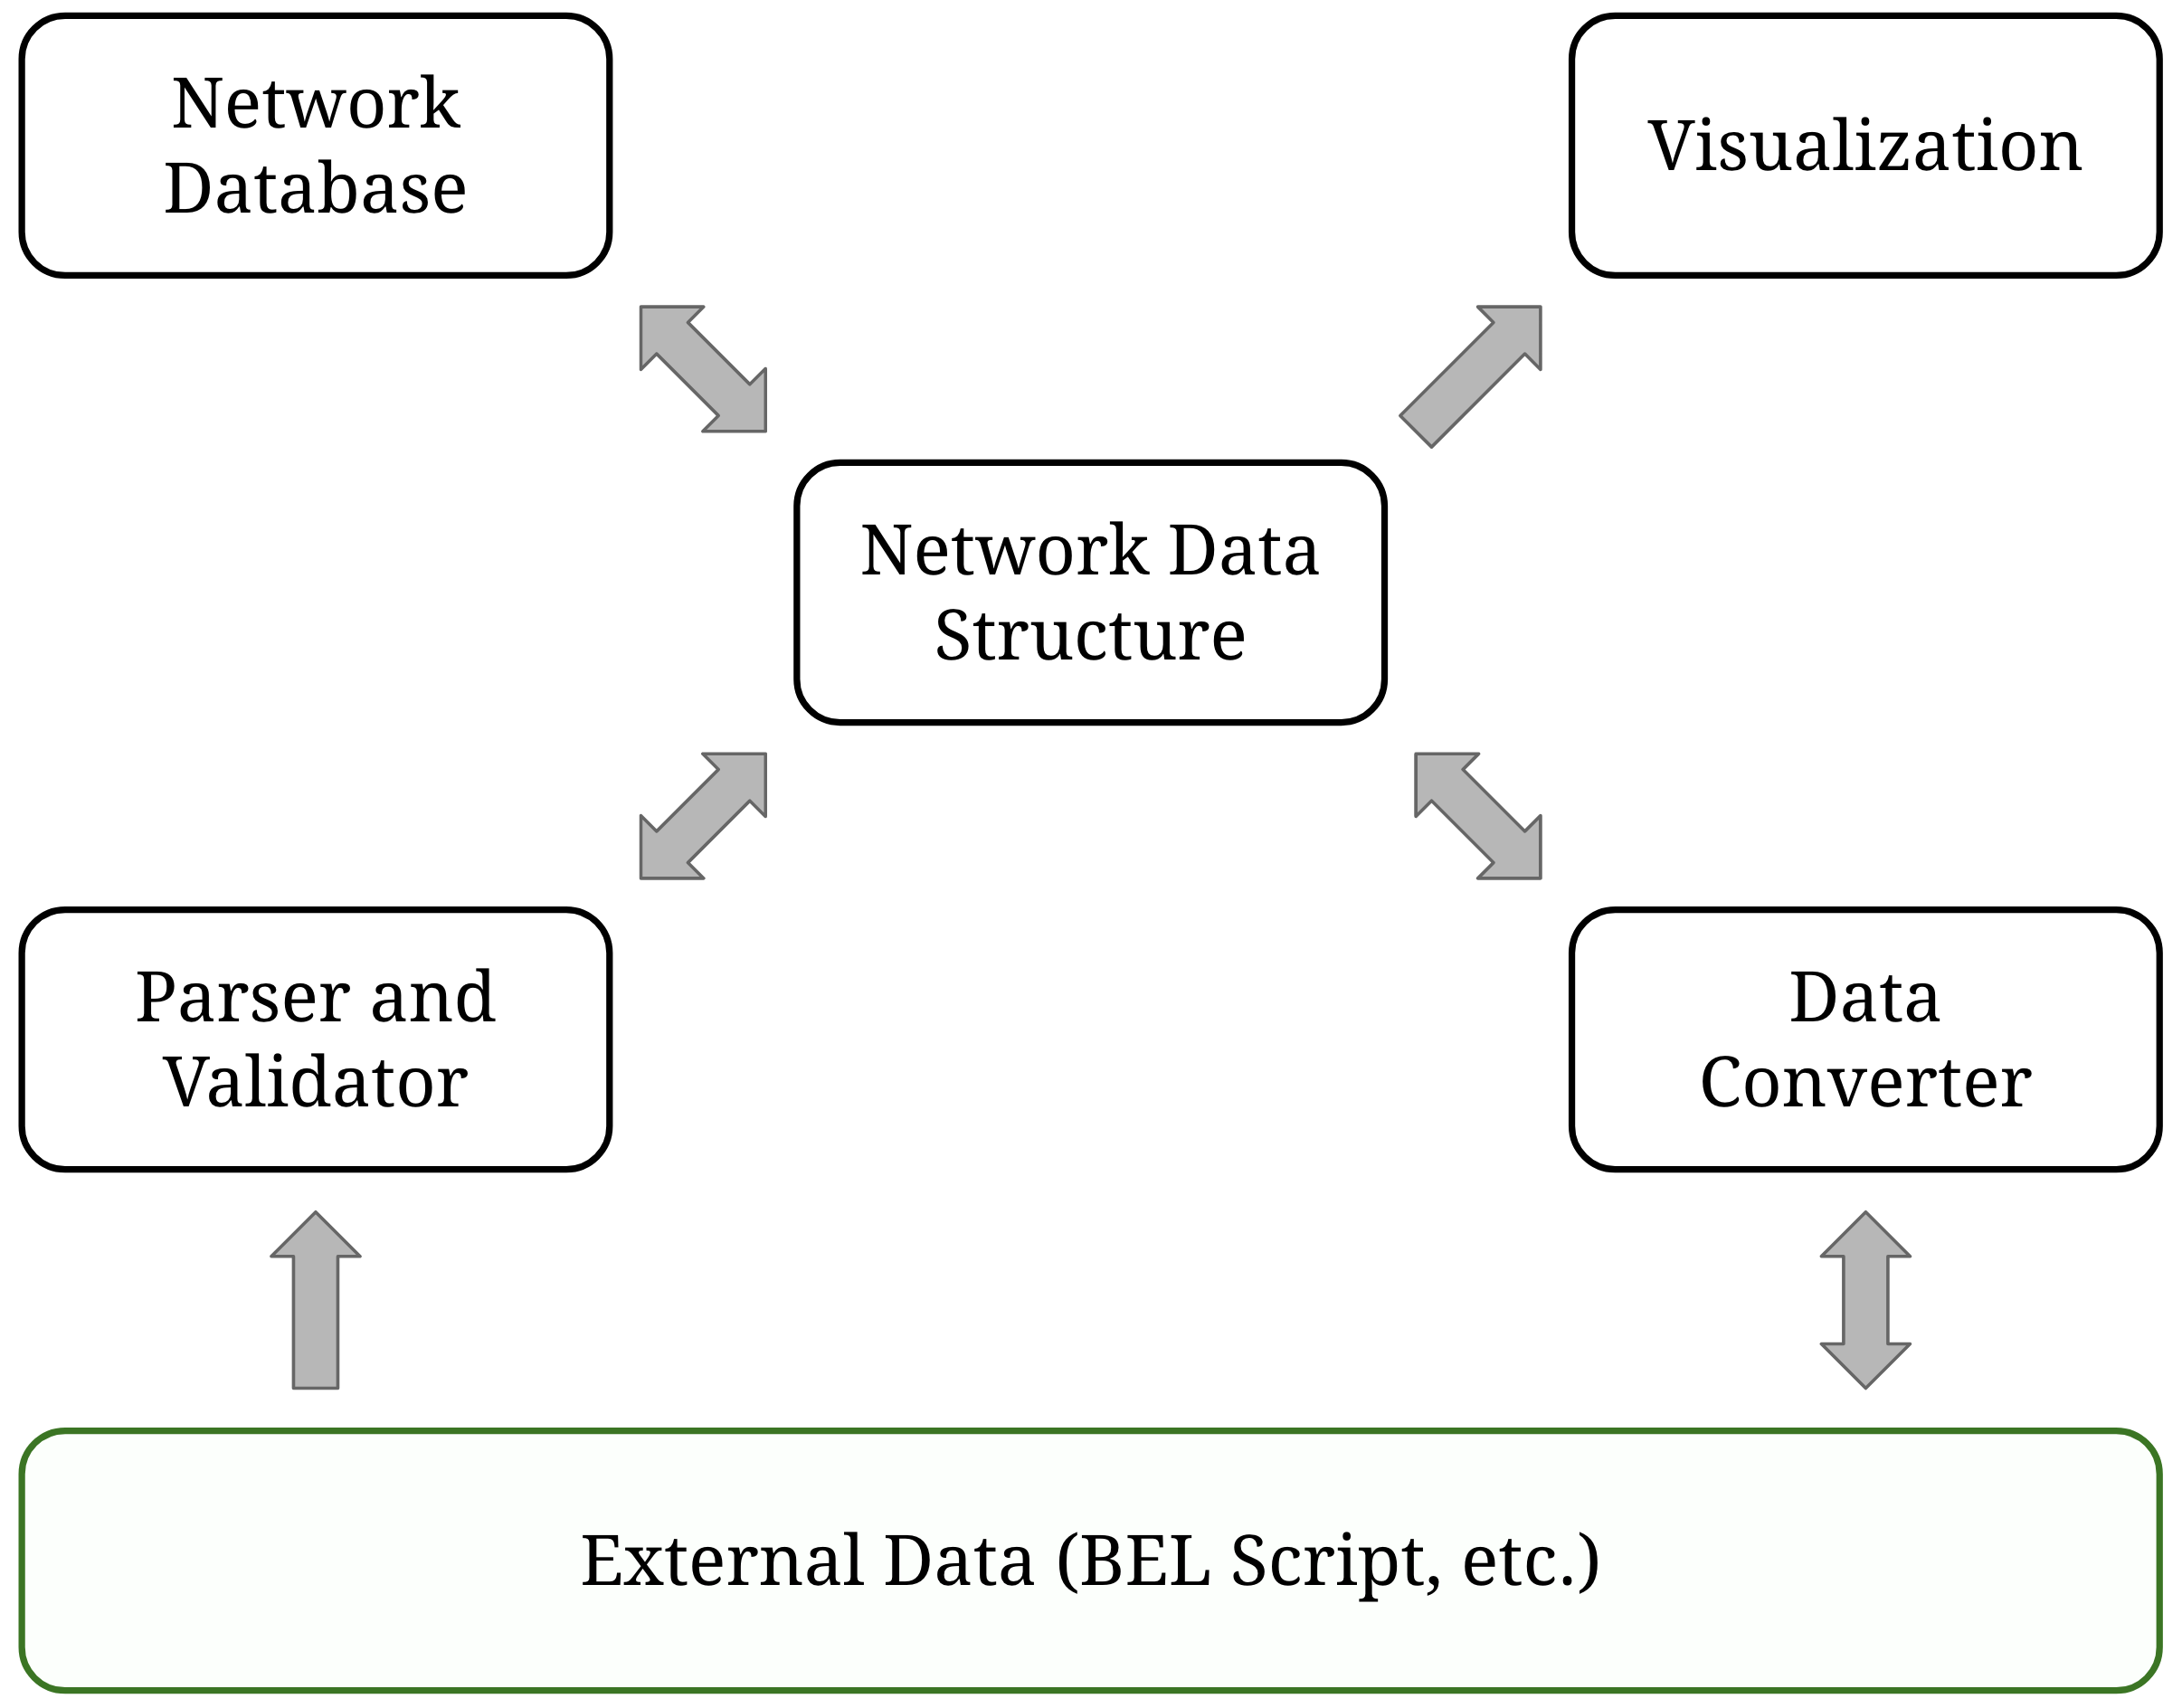
\includegraphics[width=120mm]{images/pybel_components.png}}
\caption[The PyBEL Software Architecture]{The PyBEL software package consists of five main parts: (1) the data container, (2) the parser and validator, (3) the network database, (4) the data converter, and (5) visualization. Arrows represent the direction of the flow of data between components. Together, these components provide a framework for developing tools for exploration and analytics.}
\label{Fig:pybel_components}
\end{figure}

\subsection{Network Data Container}
While a graph refers to an abstraction for a set of objects (i.e. nodes) and their relations (i.e. edges), its instantiation in a real-world application is often called a network. PyBEL implements a directed multigraph (i.e. a graph whose edges have directionality and any given pair of nodes may have multiple edges) that maps the biological entities and concepts in the subjects and objects of \ac{BEL} relations to nodes in a network and their relations, with corresponding metadata, to edges. It extends the MultiDiGraph class from NetworkX, a Python package for manipulation of networks \cite{Hagberg2008}, to enable users direct access to their suite of network algorithms and provide additional tools to develop them into biologically meaningful analyses. While no-SQL database systems like Neo4J \cite{neo4j} are also able to store and make increasingly complicated queries over networks, they inherently lack the extensibility of data structures native to programming languages like Python that can be extended and directly manipulated.

Additional information can be annotated on each of the node, edge, and graph levels. This can allow of the integration of tabular information (i.e. differential gene expression on nodes or $IC_{50}$ values for edges representing inhibition experiments of chemicals on enzymes). Network-level annotations allows for storage of all relevant provenance information related to curation and namespace definitions in order to enable semantic data integration with other network and tabular data sources. 

\subsection{Parsing and Validation}

The parser combines components for performing tokenization, lexical analysis, parsing, and validation on each of the three sections of BEL Script. Each was implemented using the internal domain-specific language provided by the PyParsing \cite{pyparsing} Python package because of its exceptional speed, ease of writing compared to regular expressions, and ability to register callbacks for different language features. One callback annotates the entries in the document metadata section to a network instance while another downloads and stores the resources referenced in the definitions section. The relations section has two main callbacks; one to maintain a list of current annotations from SET statements and another to parse BEL relations (Figure 4C-D) and populate a network instance with the corresponding nodes, edges, and their metadata from the current internal state.  

While relations' syntax is implicitly validated by the implementation of BEL in PyParsing, the semantics of their subjects' and objects' identifiers are validated with the references stored earlier. Finally, feedback is provided to users with thorough error analyses to support thoughtful re-curation, which could lead to more robust knowledge assemblies and enable more reproducible science.

\subsection{Network and Edge Store}

PyBEL uses a relational database to cache external namespaces and pre-parsed networks to improve the speed of validation and access to data. While relational databases are not generally appropriate for applying network algorithms, they do provide indexing functionality that enables complicated queries and filters over the nodes, edges, and metadata of increasingly large collections of networks. For example, this could enable the identification of intersections and potential cross-talk in different disease-specific networks. SQLAlchemy \cite{sqlalchemy}, a popular object-relational mapper, was used to maintain the database schema, transport the results of queries to PyBEL, and enable integration of external relational databases. Additionally, SQLAlchemy supports both fully-featured relational database management systems as well as SQLite \cite{sqlite} for a zero-configuration option. 

\subsection{Data Converter}

Lossless conversion protocols were implemented for common file formats including Node-Link \ac{JSON}, \ac{JGIF}, CX, and Python Pickle as well as for multiple common database formats including \ac{SQL}, Neo4J, and the \ac{NDEx} (Table 1). Additional lossy exporters were provided to \ac{CSV}, \ac{SIF}, Excel, \ac{XGMML}, and \ac{GSEA} and \ac{GRP} to facilitate usage in other programs (Table 2). Notably, implementing a RDF converter was deferred until improvements are made to the existing BEL to RDF mapping and its documentation \cite{openbelrdf}.

\begin{table}
\centering
\caption[PyBEL Interconversion Formats]{Multiple lossless converters are provided to common file formats and databases. Full descriptions of the programmatic API can be found at http://pybel.readthedocs.io/en/latest/io.html}
\label{tab:conversion}
\def\arraystretch{1.5}
\begin{tabular}{p{2cm} p{12cm}}
Format & Usage \\
\hline
BEL Script & Output to BEL scripts results in upgrade of statements from BEL v1.0 and a standardized formatting. \\
Binary & Using Python’s pickle module, pre-parsed BEL Script can be stored as binary data for fast loading, storage in databases, and transfer via network protocols. \\
Node-Link & Node-Link \cite{nodelink} is the standard \ac{JSON} format for many web-based network visualization tools, including D3.js \cite{d3js}. Output is facilitated by standard code provided by NetworkX. \\
JGIF & \ac{JGIF} \cite{jsongraphformat} is defined by a schema that is nearly a proper subset of the Node Link format. Conversion with this format provides compatibility with other software and repositories, such as the Causal Biological Network Database \cite{Talikka2015}. \\
CX & CX \cite{cxmodel} is an aspect-oriented network interchange format encoded in JSON with a format inspired by the JSON-LD \cite{jsonld} encoding of RDF. It is primarily used by the \ac{NDEx} and more recent versions of Cytoscape. \\
NDEx & PyBEL contains wraps the \ac{NDEx} Python client \cite{ndexpython} for seamless upload/download to the \ac{NDEx} in the CX format. \\
SQL & SQLAlchemy is used to make abstract queries over the nodes and edges of a collection of networks. \\
Neo4J & Neo4J  is a graph database that enables complex graph queries with the Cypher querying language.
\end{tabular}
\end{table}

\begin{table}
\centering
\caption[PyBEL Export Formats]{Exporters to lossy and irretrievable formats are provided to promote usability in other programs.}
\label{tab:lossy_exporters}
\def\arraystretch{1.5}
\begin{tabular}{p{2cm} p{12cm}}
Format              & Usage \\
\hline
CSV, SIF, and Excel & \ac{CSV}, \ac{SIF}, and Excel all consist of an edge list with interaction types that are suited for viewing in Excel or Cytoscape.                                                                                              \\
XGMML               & \ac{XGMML} \cite{xgmml} supersedes \ac{GML} by adding support for both node and edge annotations. Its name derives from its encoding in \ac{XML}. It can be directly imported to Cytoscape for viewing. \\
HTML                & Interactive visualizations can be produced using JSON export and D3.js. They can be embedded directly in Jupyter Notebook.                                                                                                                                                  \\
GSEA                & This export option outputs a list of genes in the \ac{GRP} format for use with the Broad Institute’s \ac{GSEA} platform \cite{Subramanian2005}.
\end{tabular}
\end{table}


\subsection{Visualization}

Networks can be exported to \ac{CSV}, \ac{SIF}, \ac{XGMML}, or CX for visualization in Cytoscape \cite{Franz2015} or uploaded to \ac{NDEx} \cite{Pratt2015} to take advantage of its viewer and simple query interface. Alternatively, PyBEL provides an interactive network explorer and visualizer that is tailored to \ac{BEL} networks (appropriate node coloring, metadata pop-ups, etc.) that can be directly embedded as \ac{HTML} in email, Jupyter Notebook \cite{Kluyver2016}, or a web application. For example, it has already been used to produce visualizations in the NeuroMMSig web server \cite{Domingo-Fernandez2017}. Figures 6-8 present the Alzheimer’s Disease Knowledge Assembly Wnt Signaling Subgraph from \ac{NeuroMMSig} in three different visualizations.

\begin{figure}
\captionsetup{format=plain}
\makebox[\textwidth]{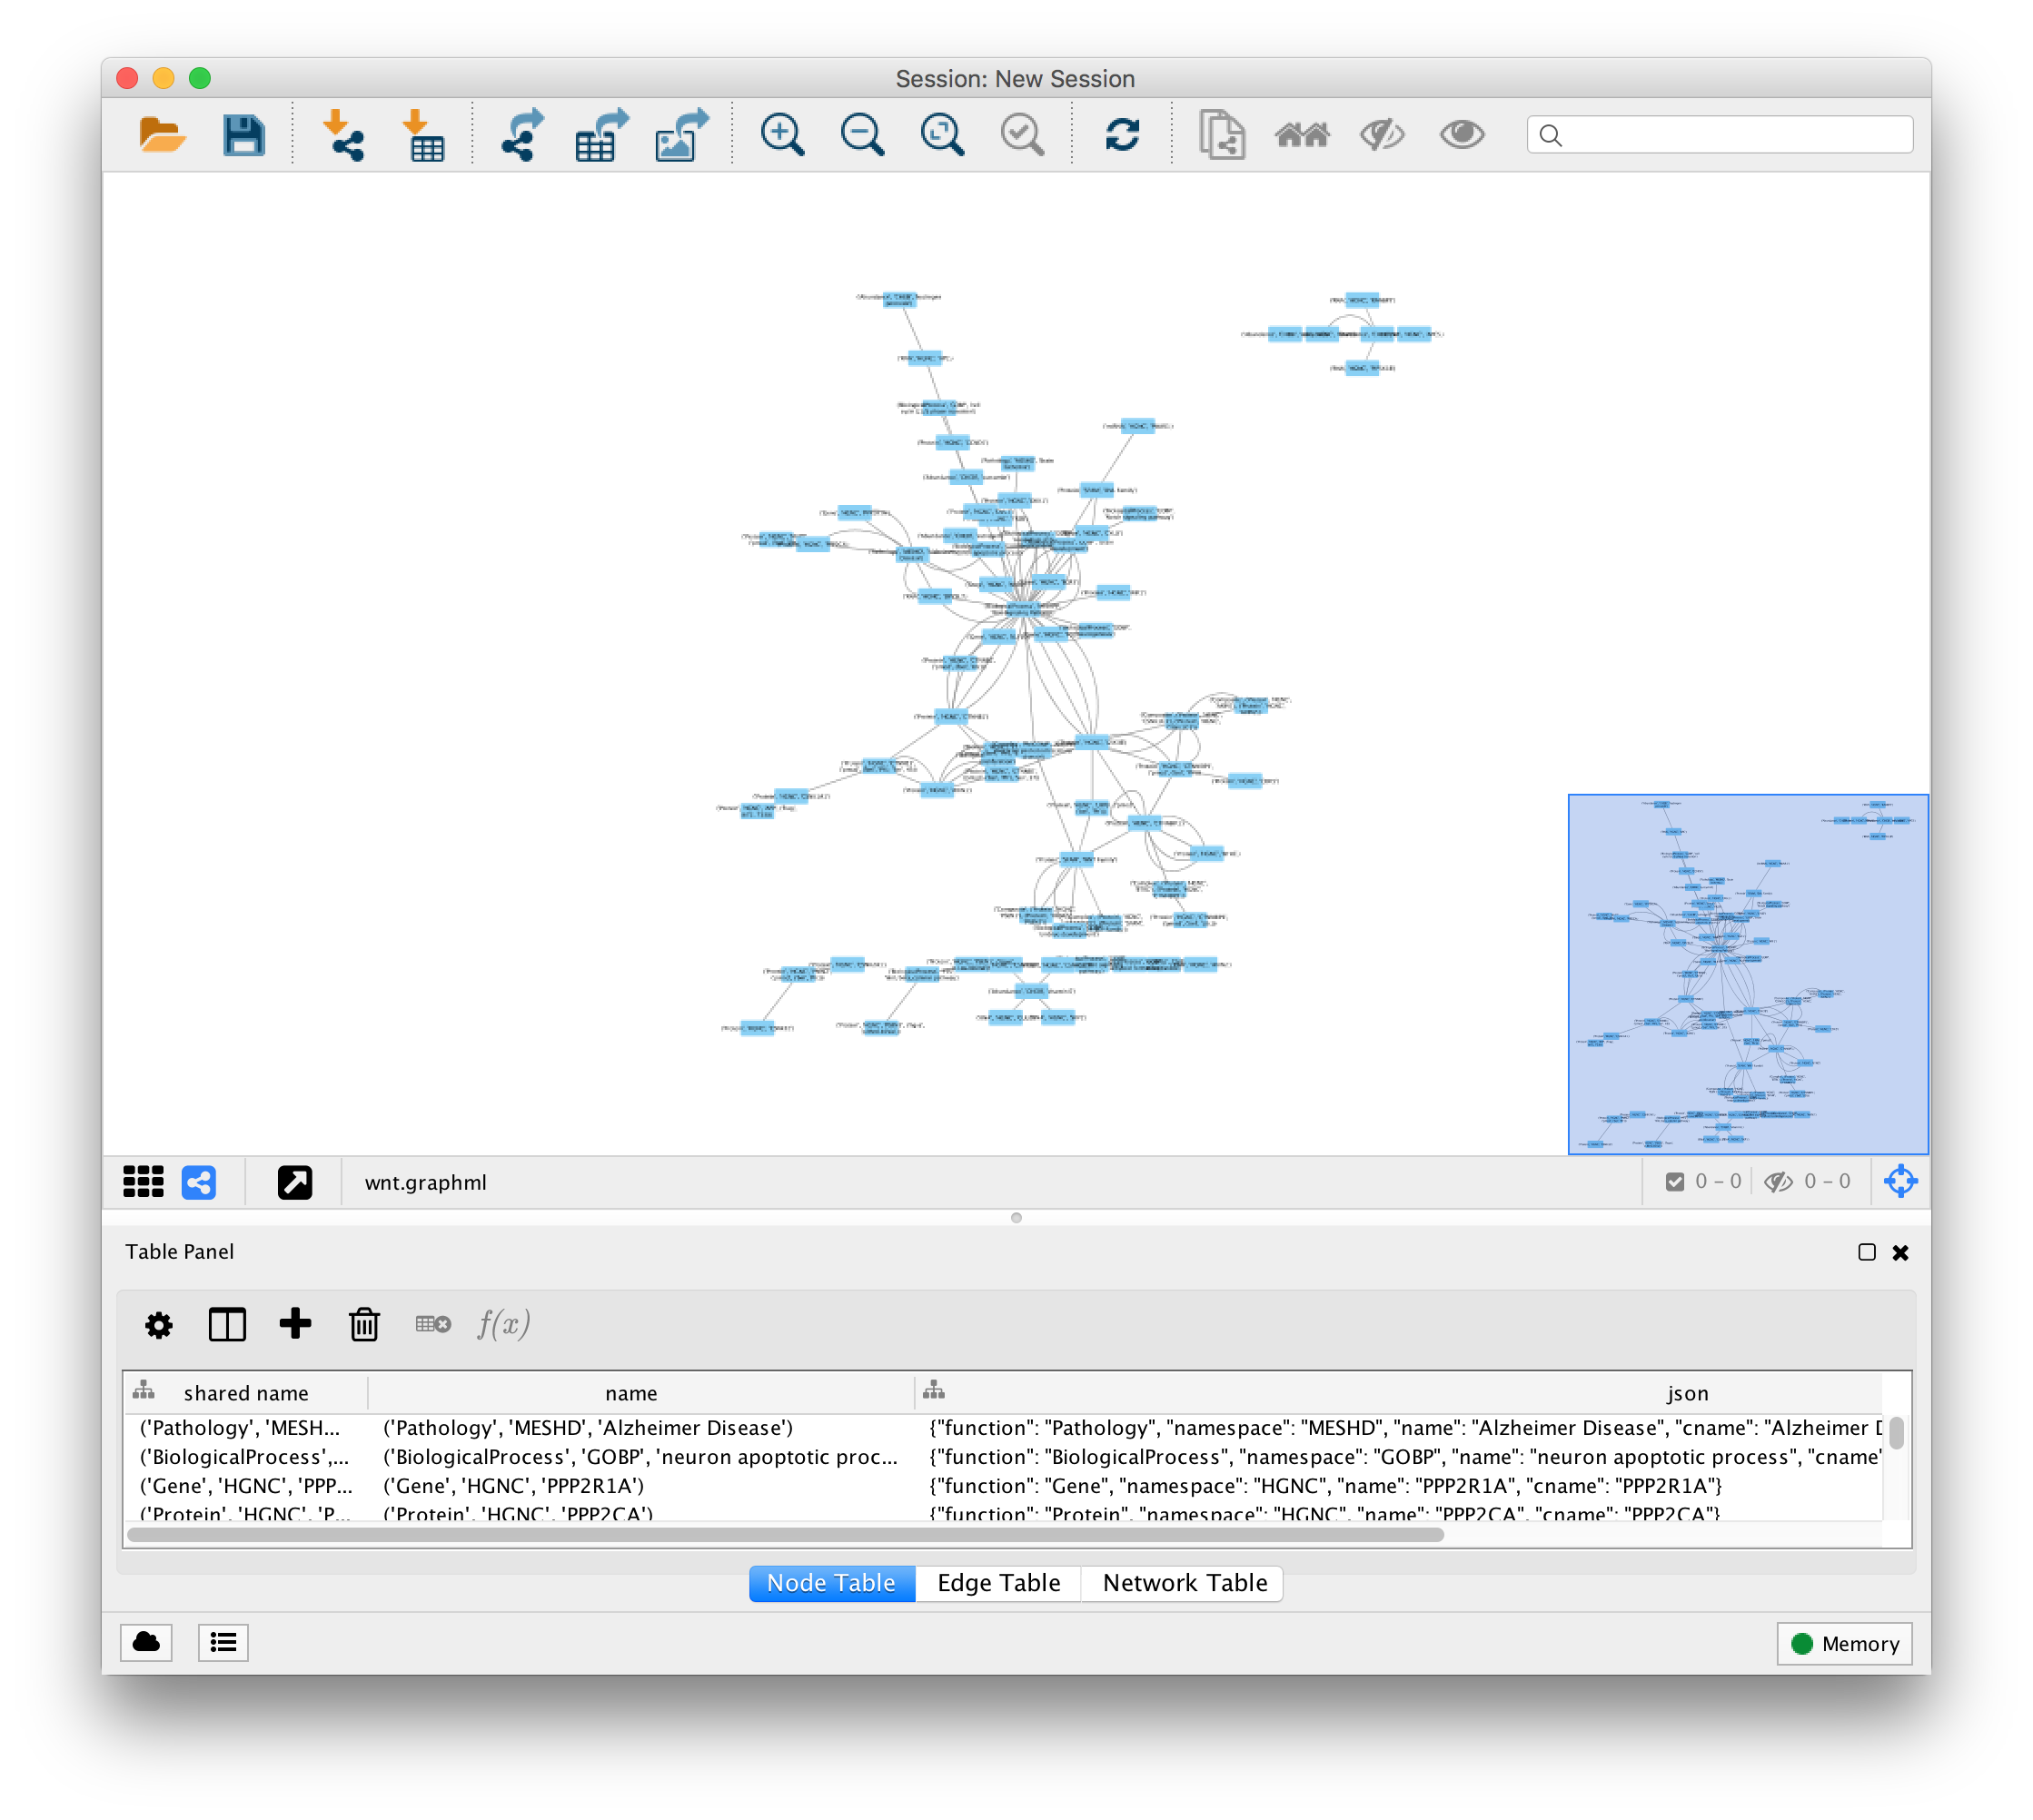
\includegraphics[width=160mm]{images/wnt_cytoscape.png}}
\caption[PyBEL Visualization of Wnt Signaling in Cytoscape]{Visualization of the Wnt Signaling Subgraph from the \ac{NeuroMMSig} Alzheimer’s Disease Knowledge Assembly with Cytoscape provides extensive styling and rudimentary access to the node and edge properties stored in PyBEL. Cytoscape also provides some network analytics functions.}
\label{Fig:wnt_cytoscape}
\end{figure}

\begin{figure}
\captionsetup{format=plain}
\makebox[\textwidth]{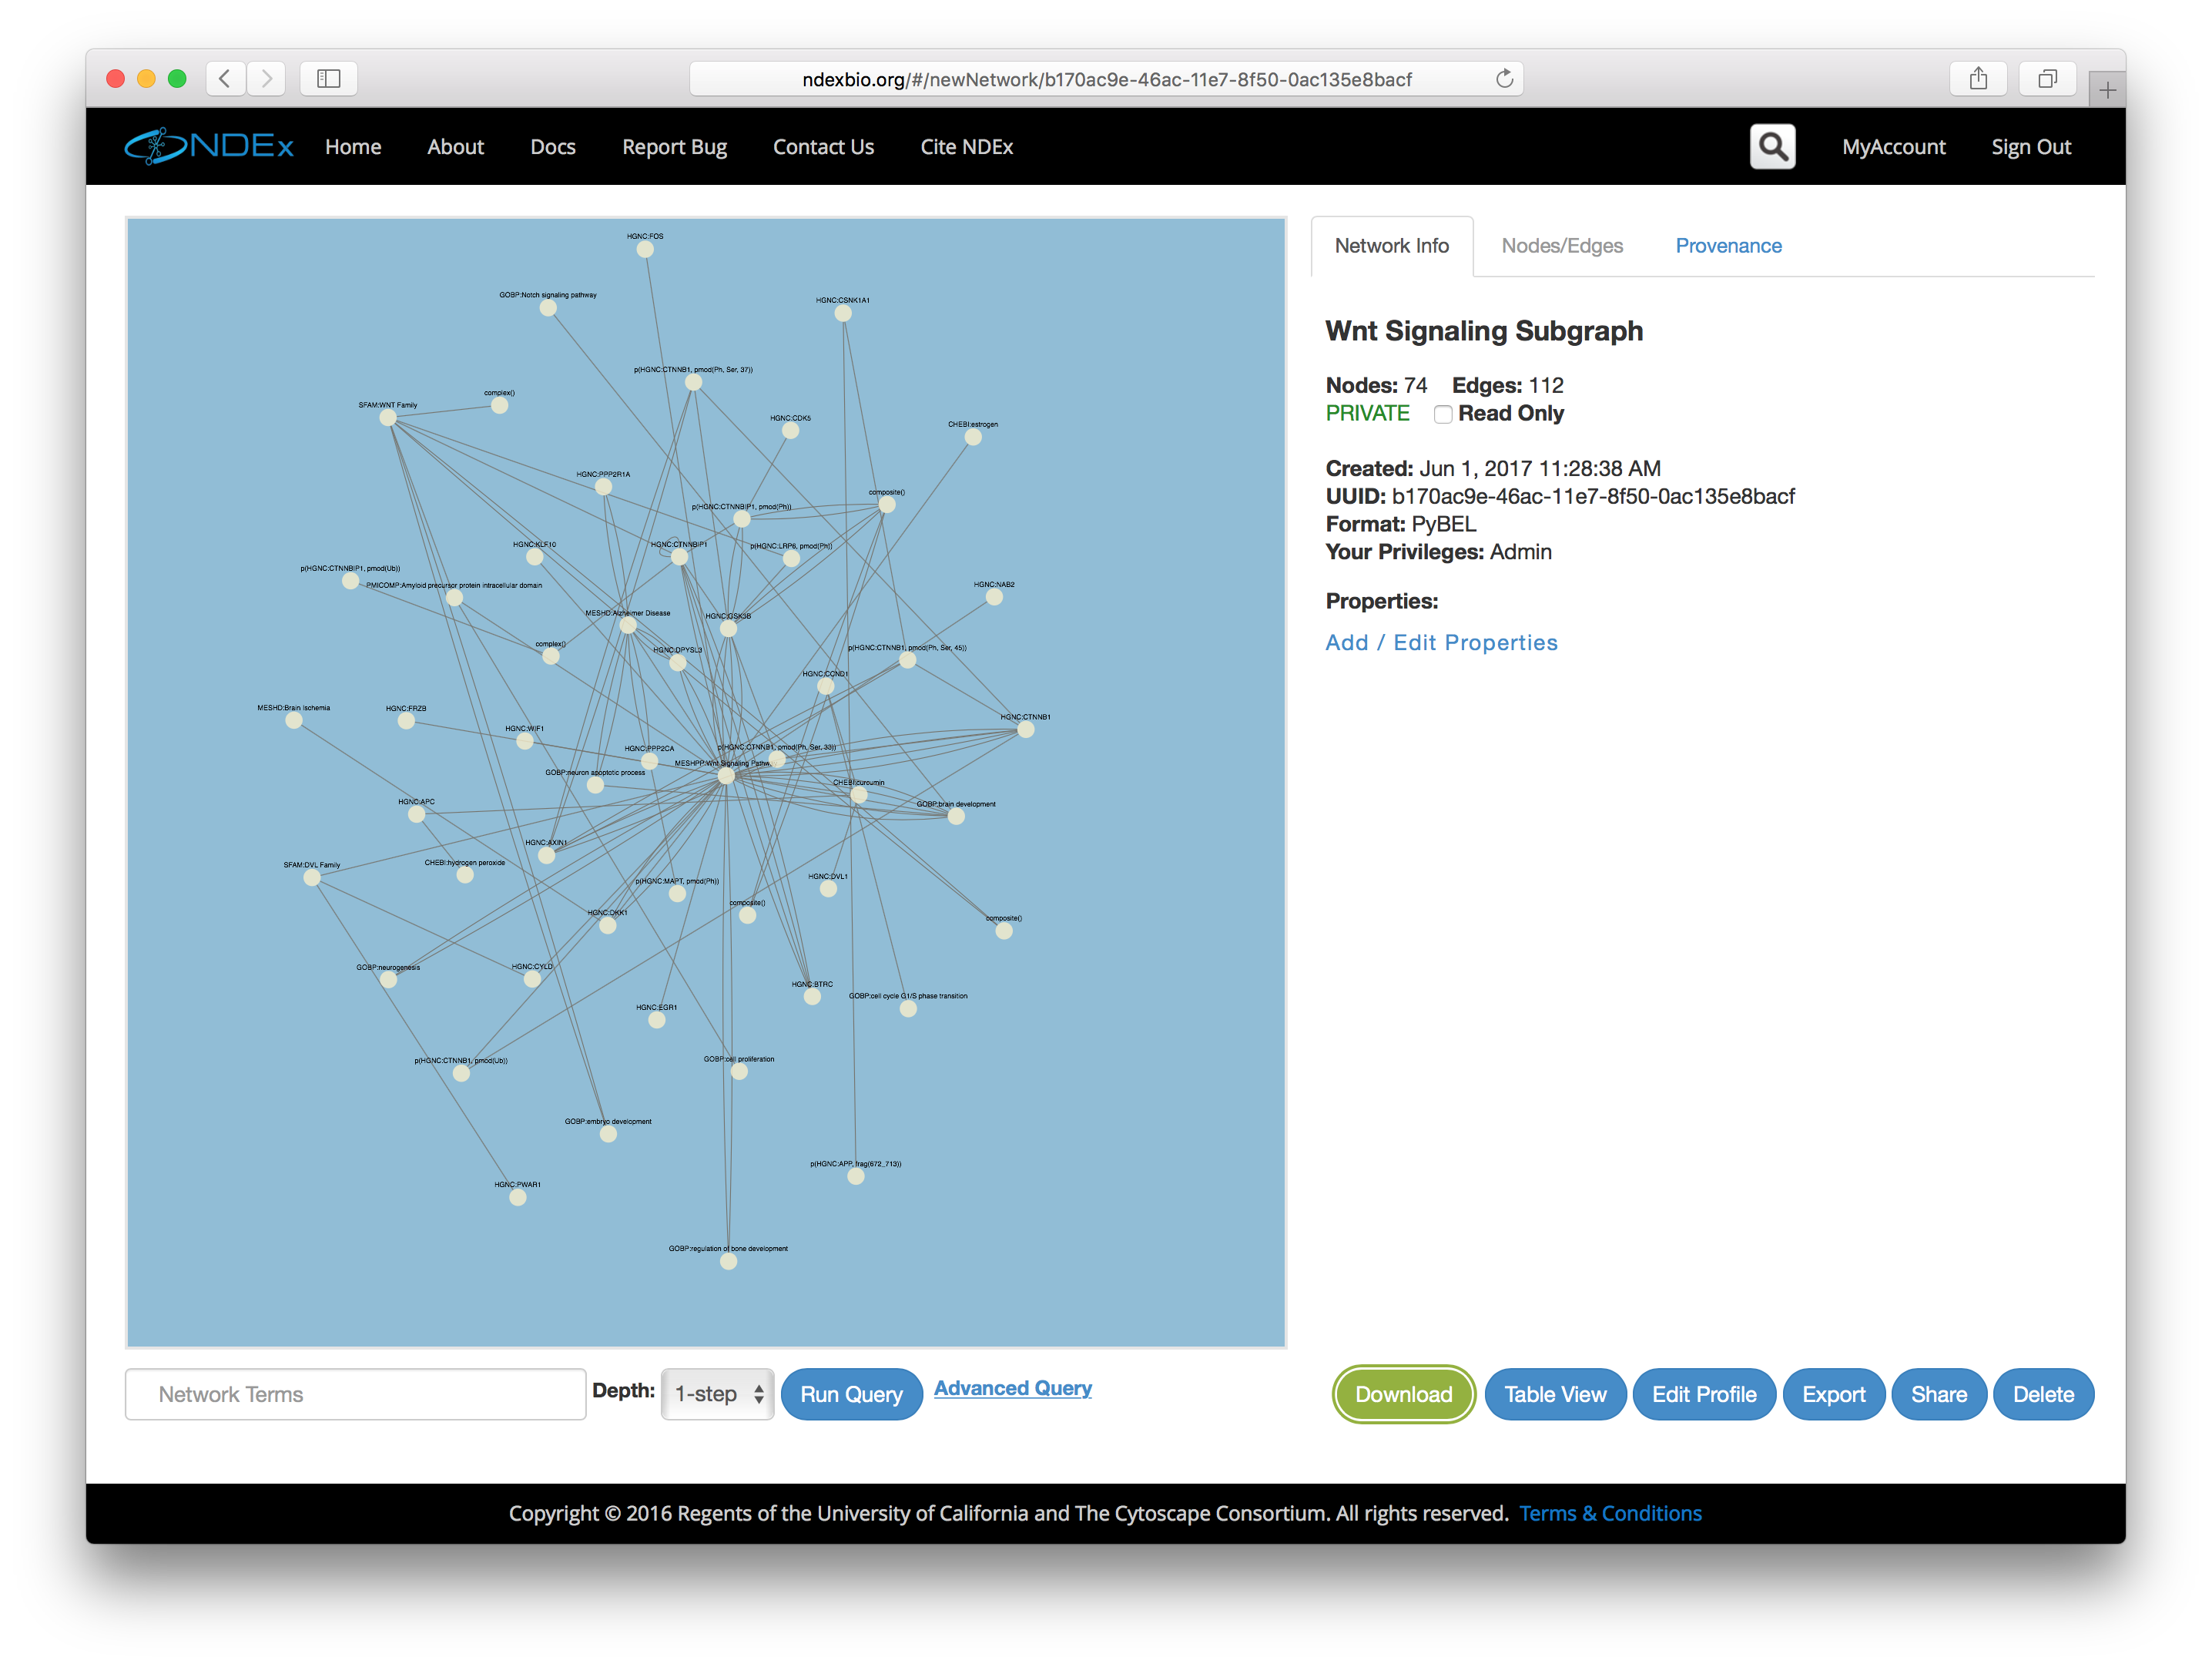
\includegraphics[width=160mm]{images/wnt_ndex.png}}
\caption[PyBEL Visualization of Wnt Signaling in NDEx]{Visualization of the Wnt Signaling Subgraph from the \ac{NeuroMMSig} Alzheimer’s Disease Knowledge Assembly with \ac{NDEx} allows users to easily share their networks.}
\label{Fig:wnt_ndex}
\end{figure}

\begin{figure}
\captionsetup{format=plain}
\makebox[\textwidth]{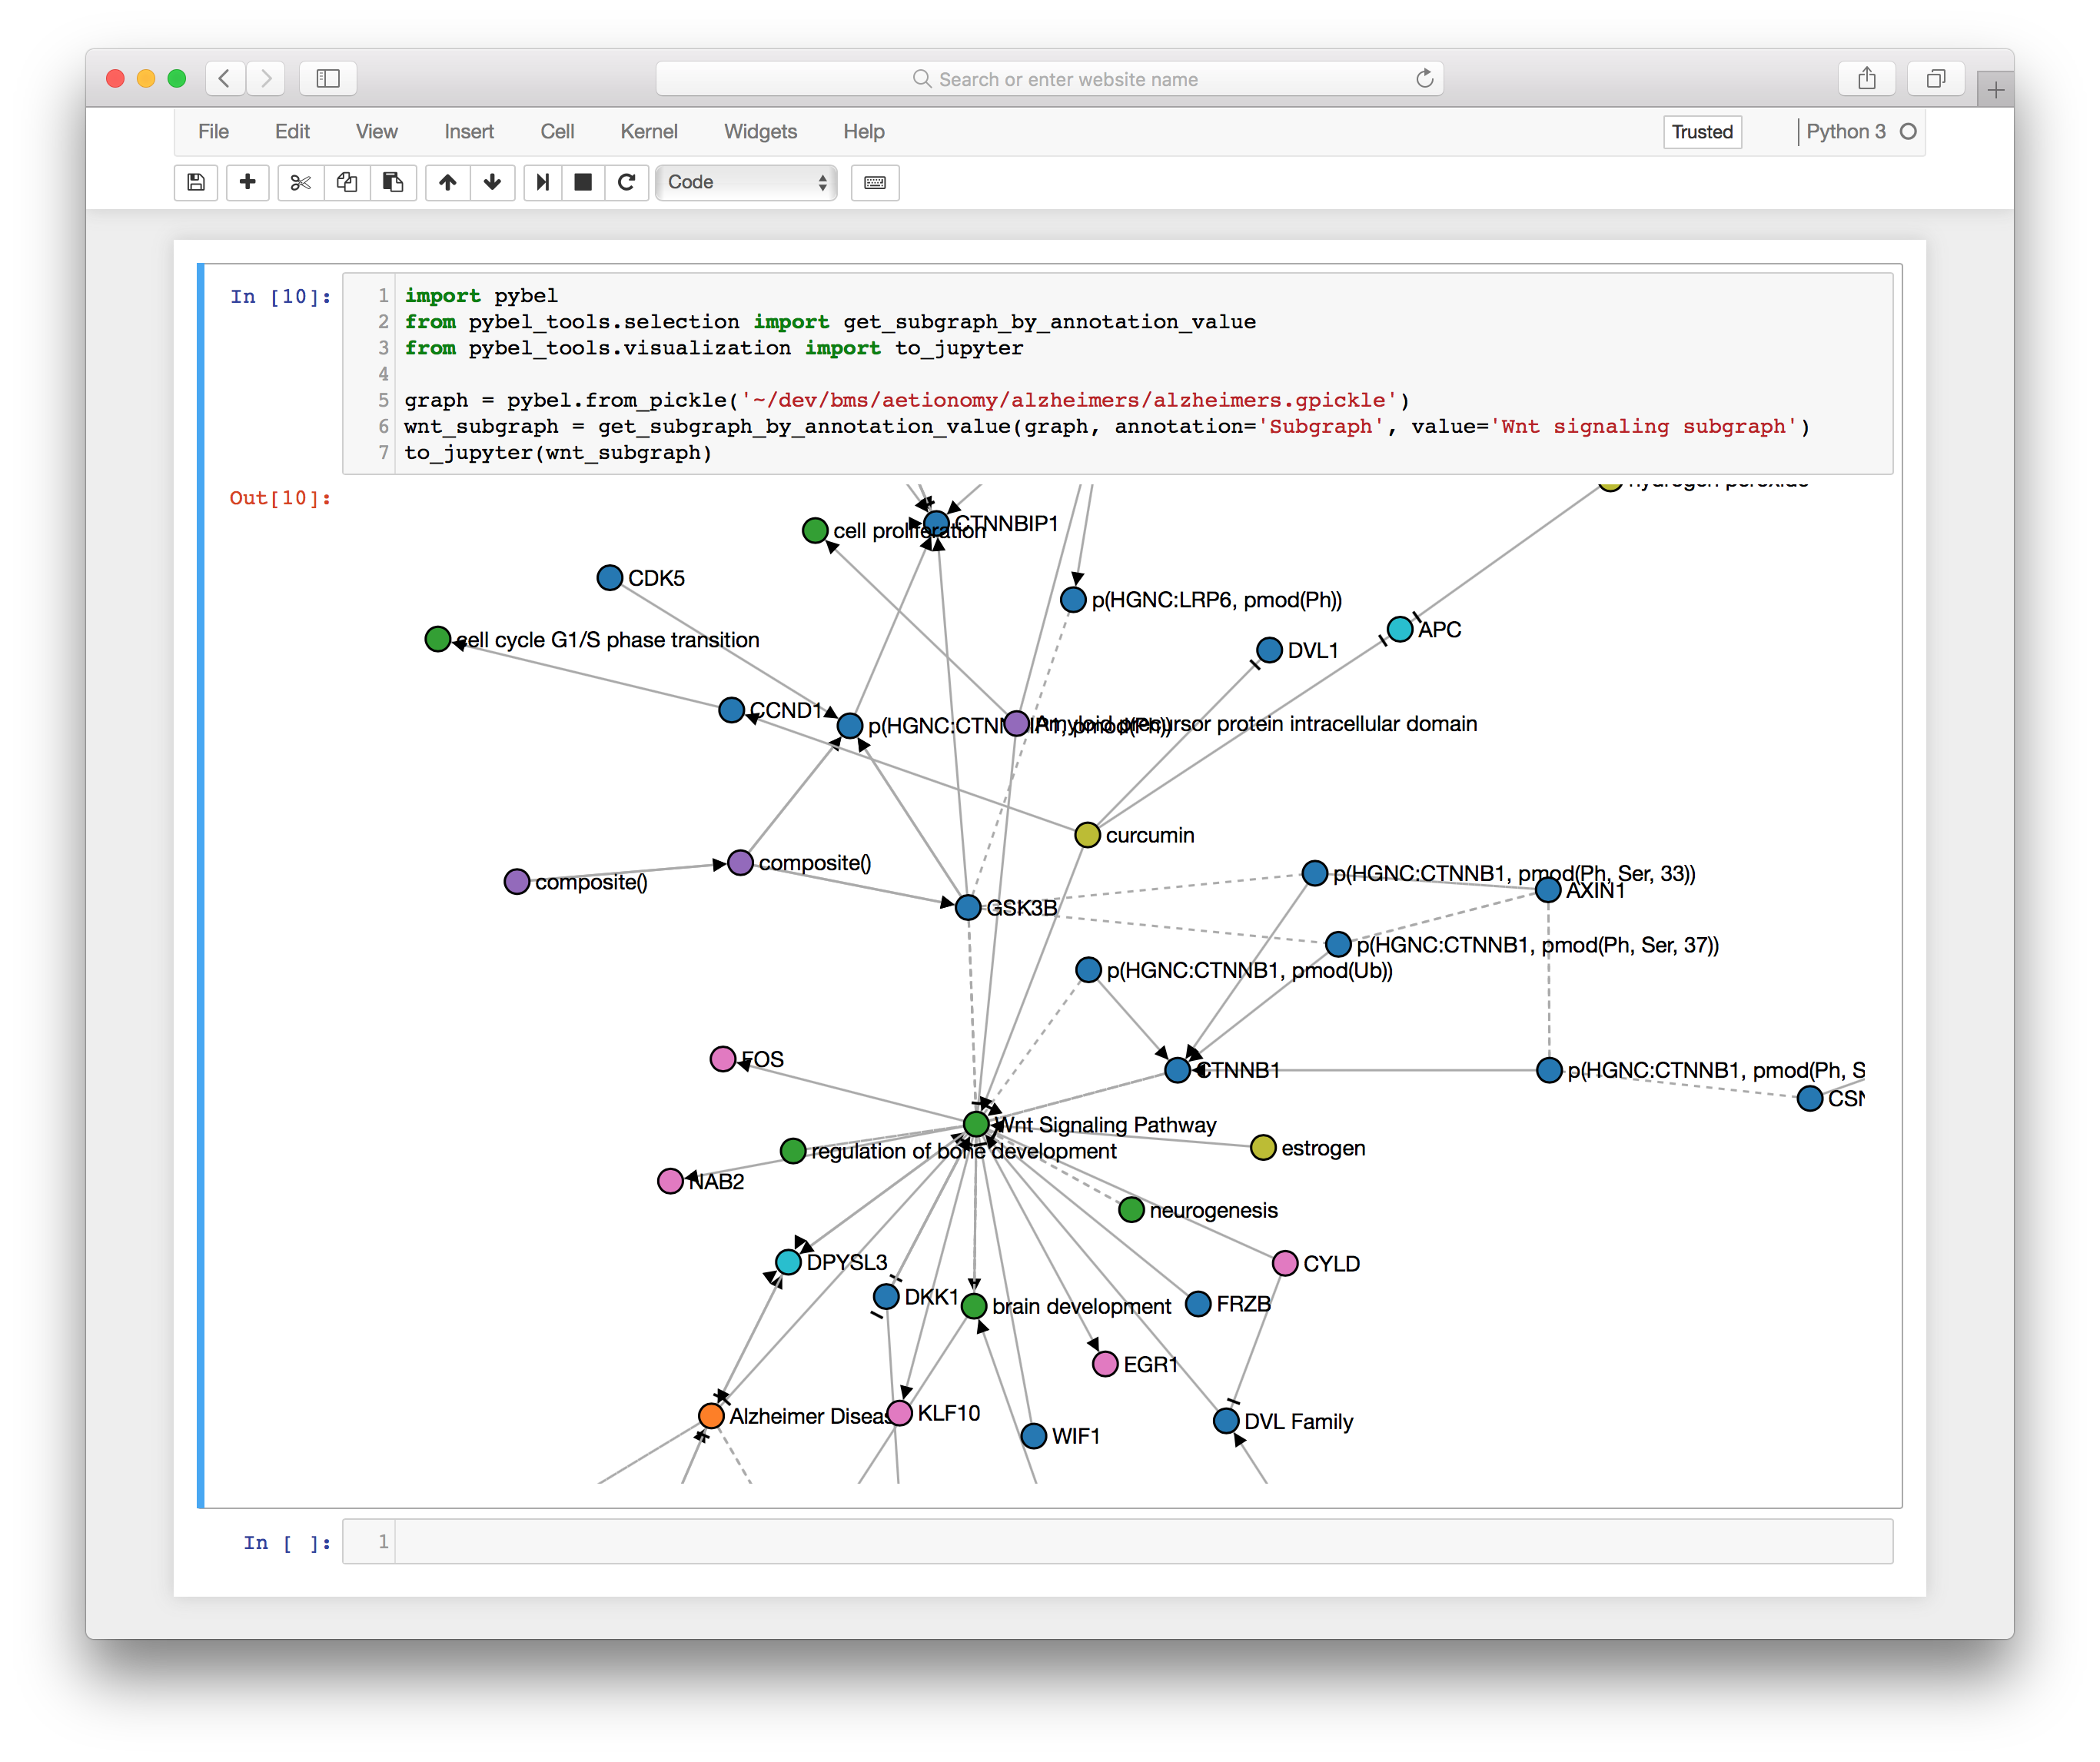
\includegraphics[width=160mm]{images/wnt_jupyter.png}}
\caption[PyBEL Visualization of Wnt Signaling in Jupyter Notebook]{Visualization of the Wnt Signaling Subgraph from the NeuroMMSig Alzheimer’s Disease Knowledge Assembly with Jupyter Notebook allows for embedding within scientific workflows.}
\label{Fig:wnt_jupyter}
\end{figure}

The visualization system from PyBEL has been built in a modular way so it can be integrated in other applications. The underlying Javascript and \ac{HTML} are written with the Jinja templating language \cite{jinja} and exposed via Python functions that can be integrated in Python code or exposed through a RESTful \ac{API}. There is ongoing work to enable users to easily visually explore the results of the \ac{BELIEF} \cite{Madan2016} and \ac{INDRA} \cite{indra} text mining pipelines. Other projects, such as the development of a web service to display and explore a knowledge base assembled for an ongoing project related to \ac{PTSD} are also currently using the PyBEL visualization to embed specific knowledge assemblies with other clinical and molecular data. Figures 9-11 present the PyBEL visualization embedded in other applications that are already in the prototype or release stage of development.

\begin{figure}
\captionsetup{format=plain}
\makebox[\textwidth]{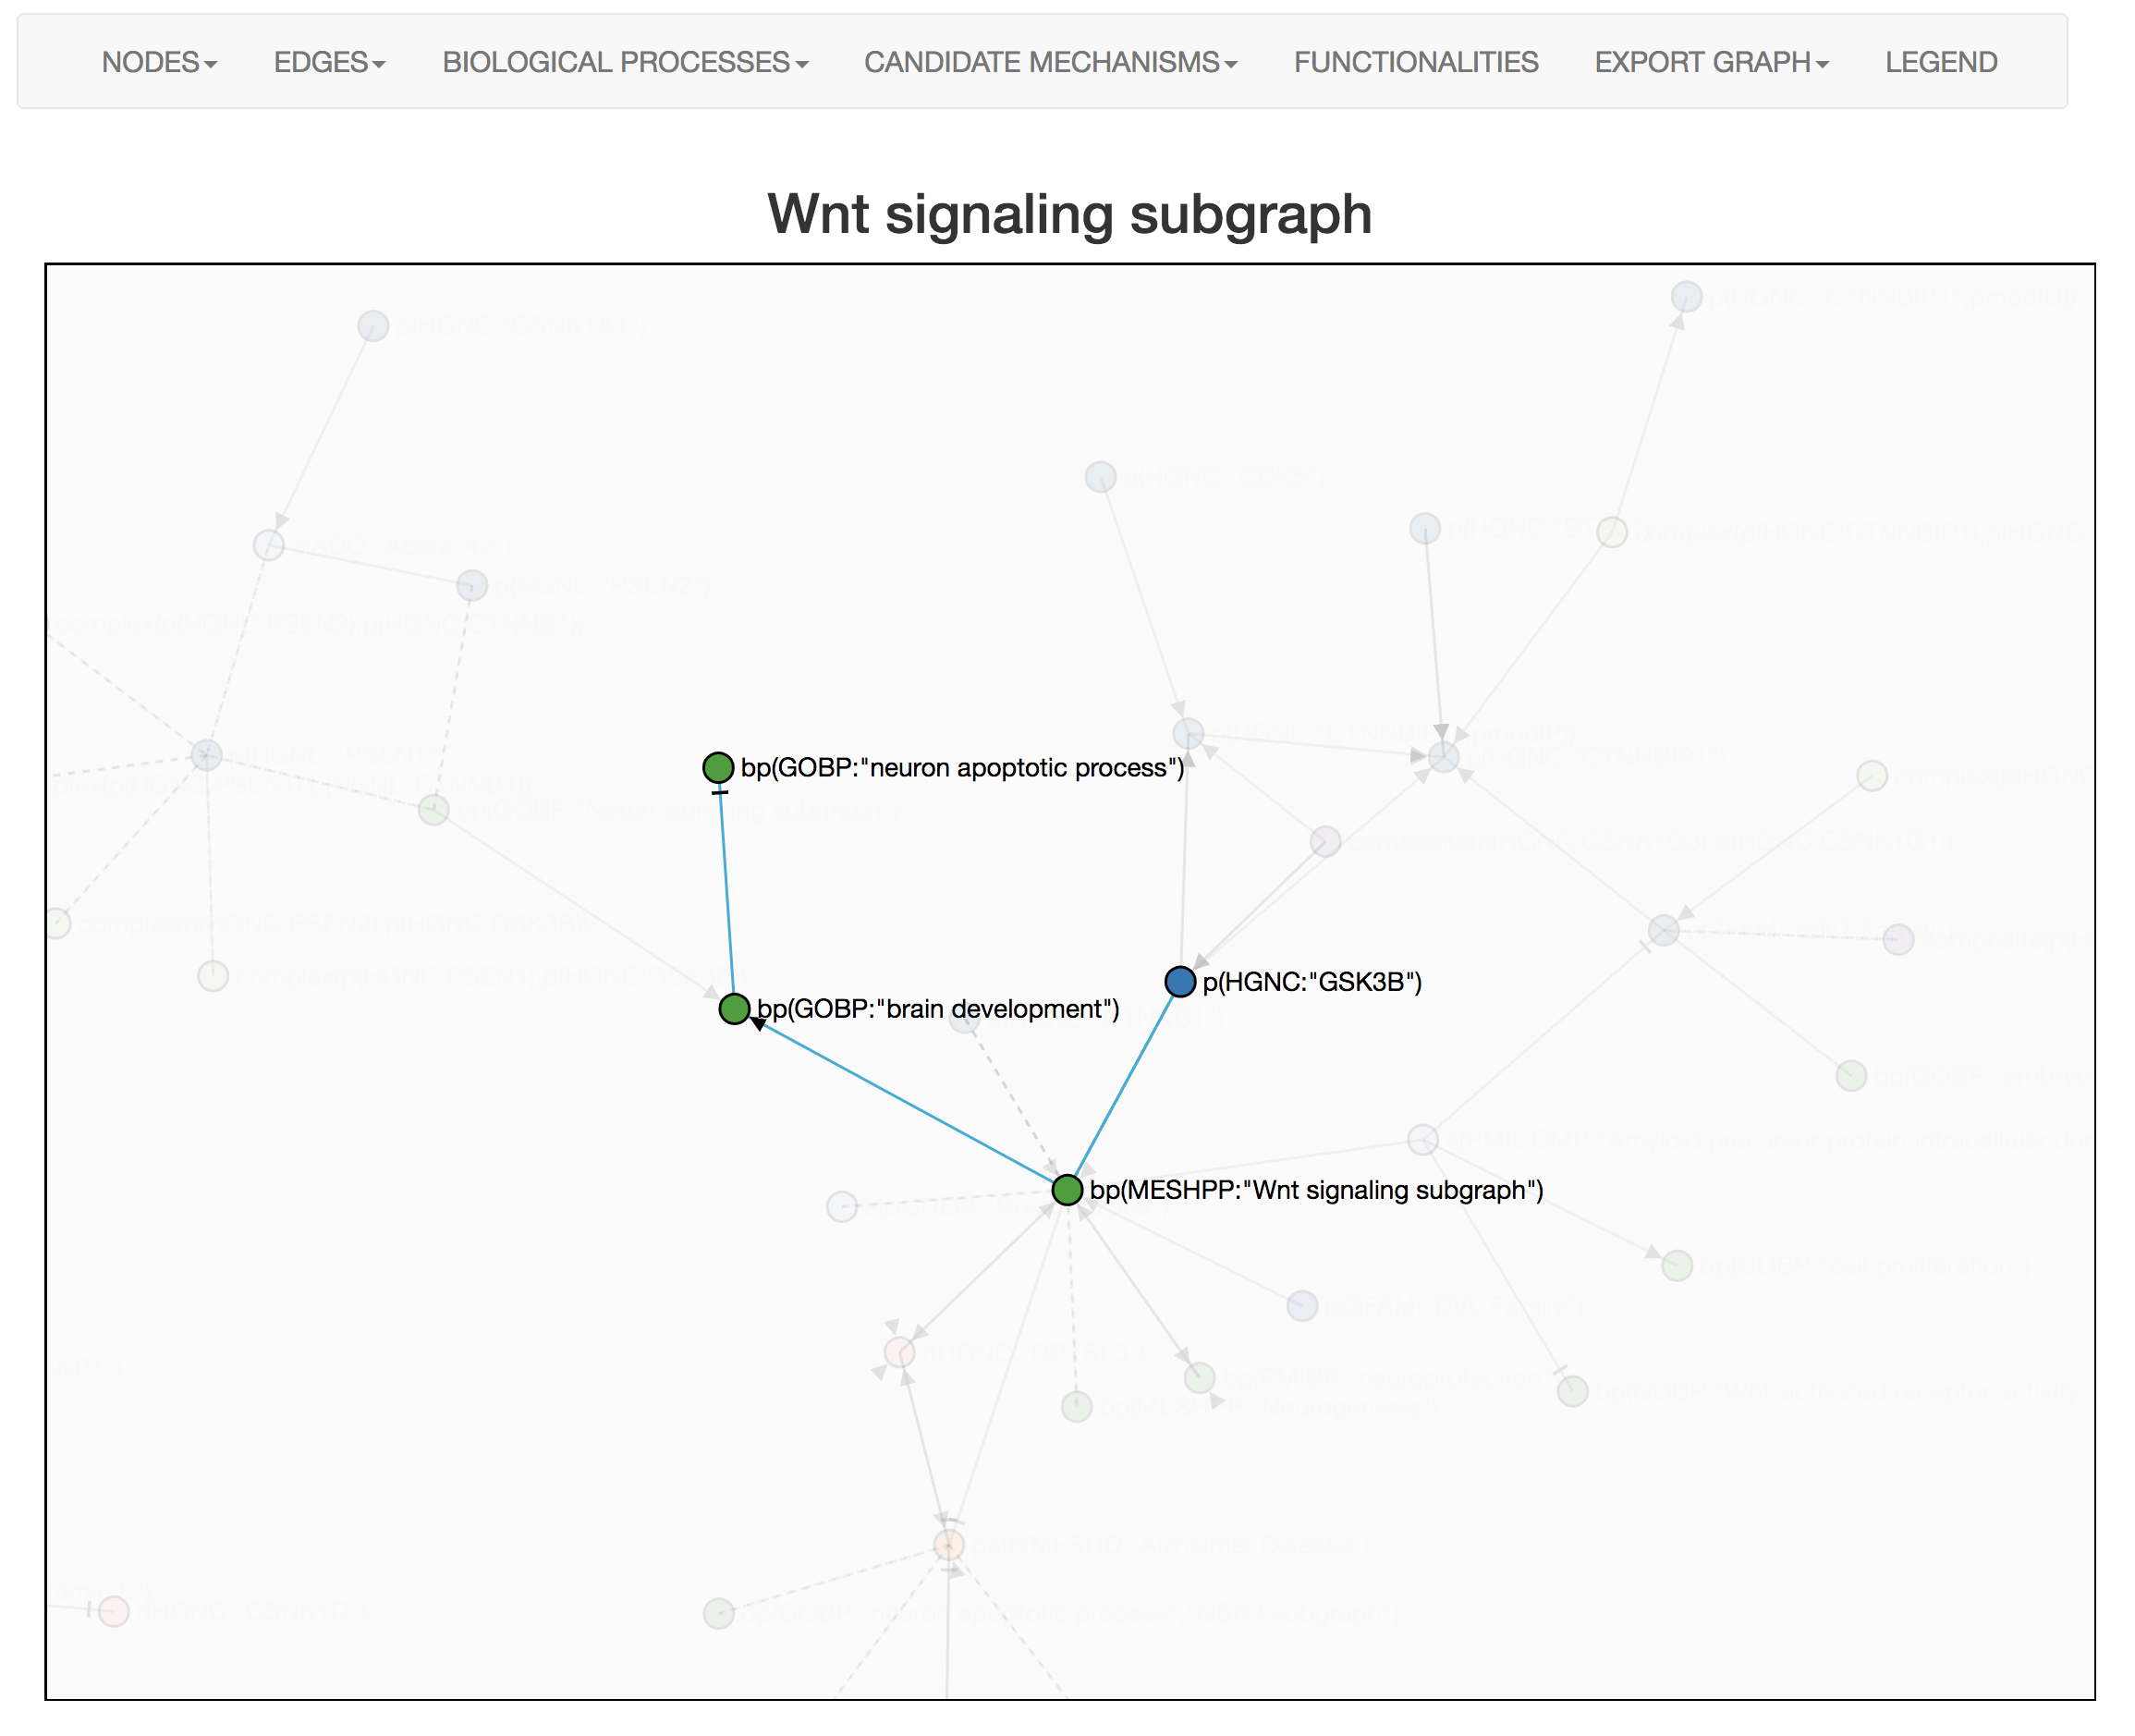
\includegraphics[width=160mm]{images/wnt_neurommsig.png}}
\caption[PyBEL Integration with the NeuroMMSig Mechanism Enrichment Server]{The NeuroMMSig Mechanism Enrichment server uses PyBEL visualization to present a downstream mechanism to the user following multi-modal mechanism enrichment.}
\label{Fig:wnt_neurommsig}
\end{figure}

\begin{figure}
\captionsetup{format=plain}
\makebox[\textwidth]{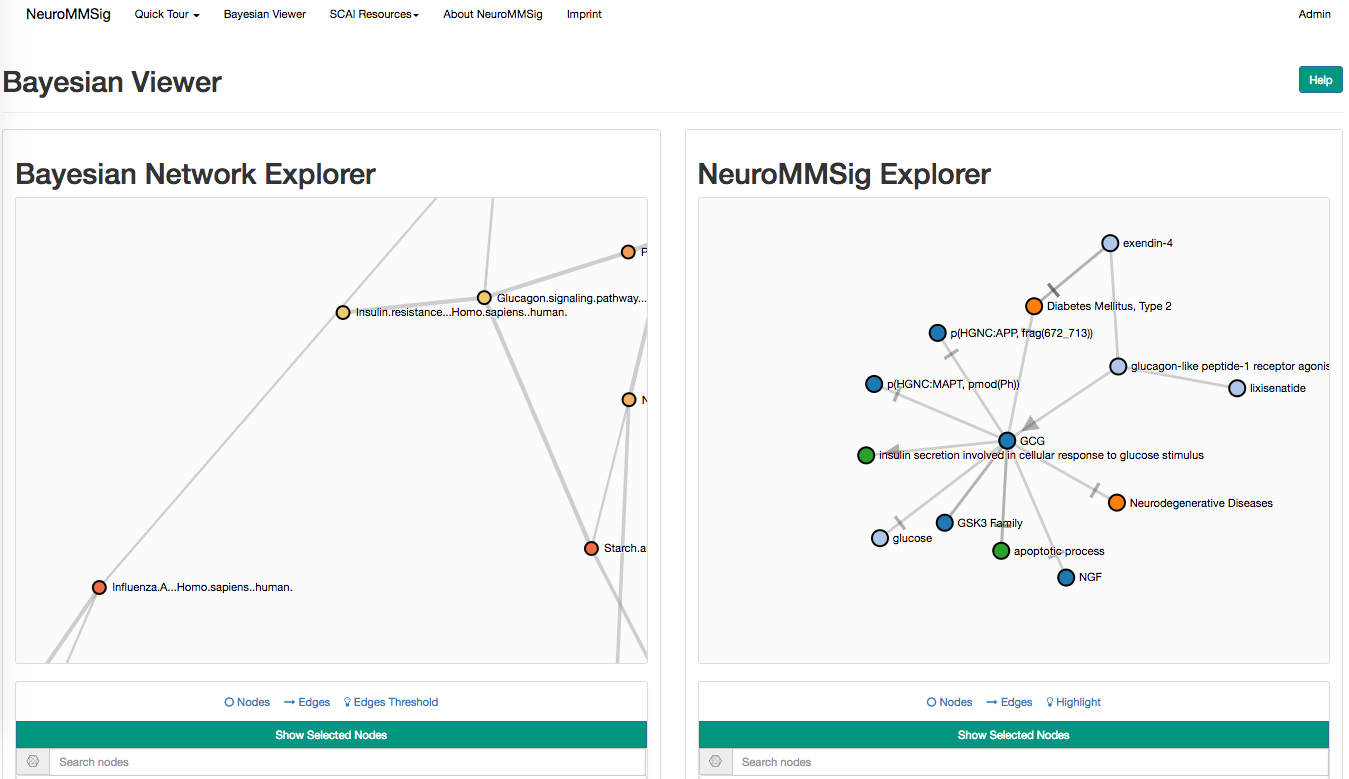
\includegraphics[width=160mm]{images/bayesian_viewer.png}}
\caption[PyBEL Integration with the NeuroMMSig Bayesian Network Explorer]{As an addition to the \ac{NeuroMMSig} Mechanism Enrichment Server, bayesian modeling techniques are used to analyze the dependencies of clinical variables, mapped to \ac{NeuroMMSig} subgraphs, and displayed in a multi-scale exploration environment using the underlying PyBEL visualization system.}
\label{Fig:bayesian_viewer}
\end{figure}

\begin{figure}
\captionsetup{format=plain}
\makebox[\textwidth]{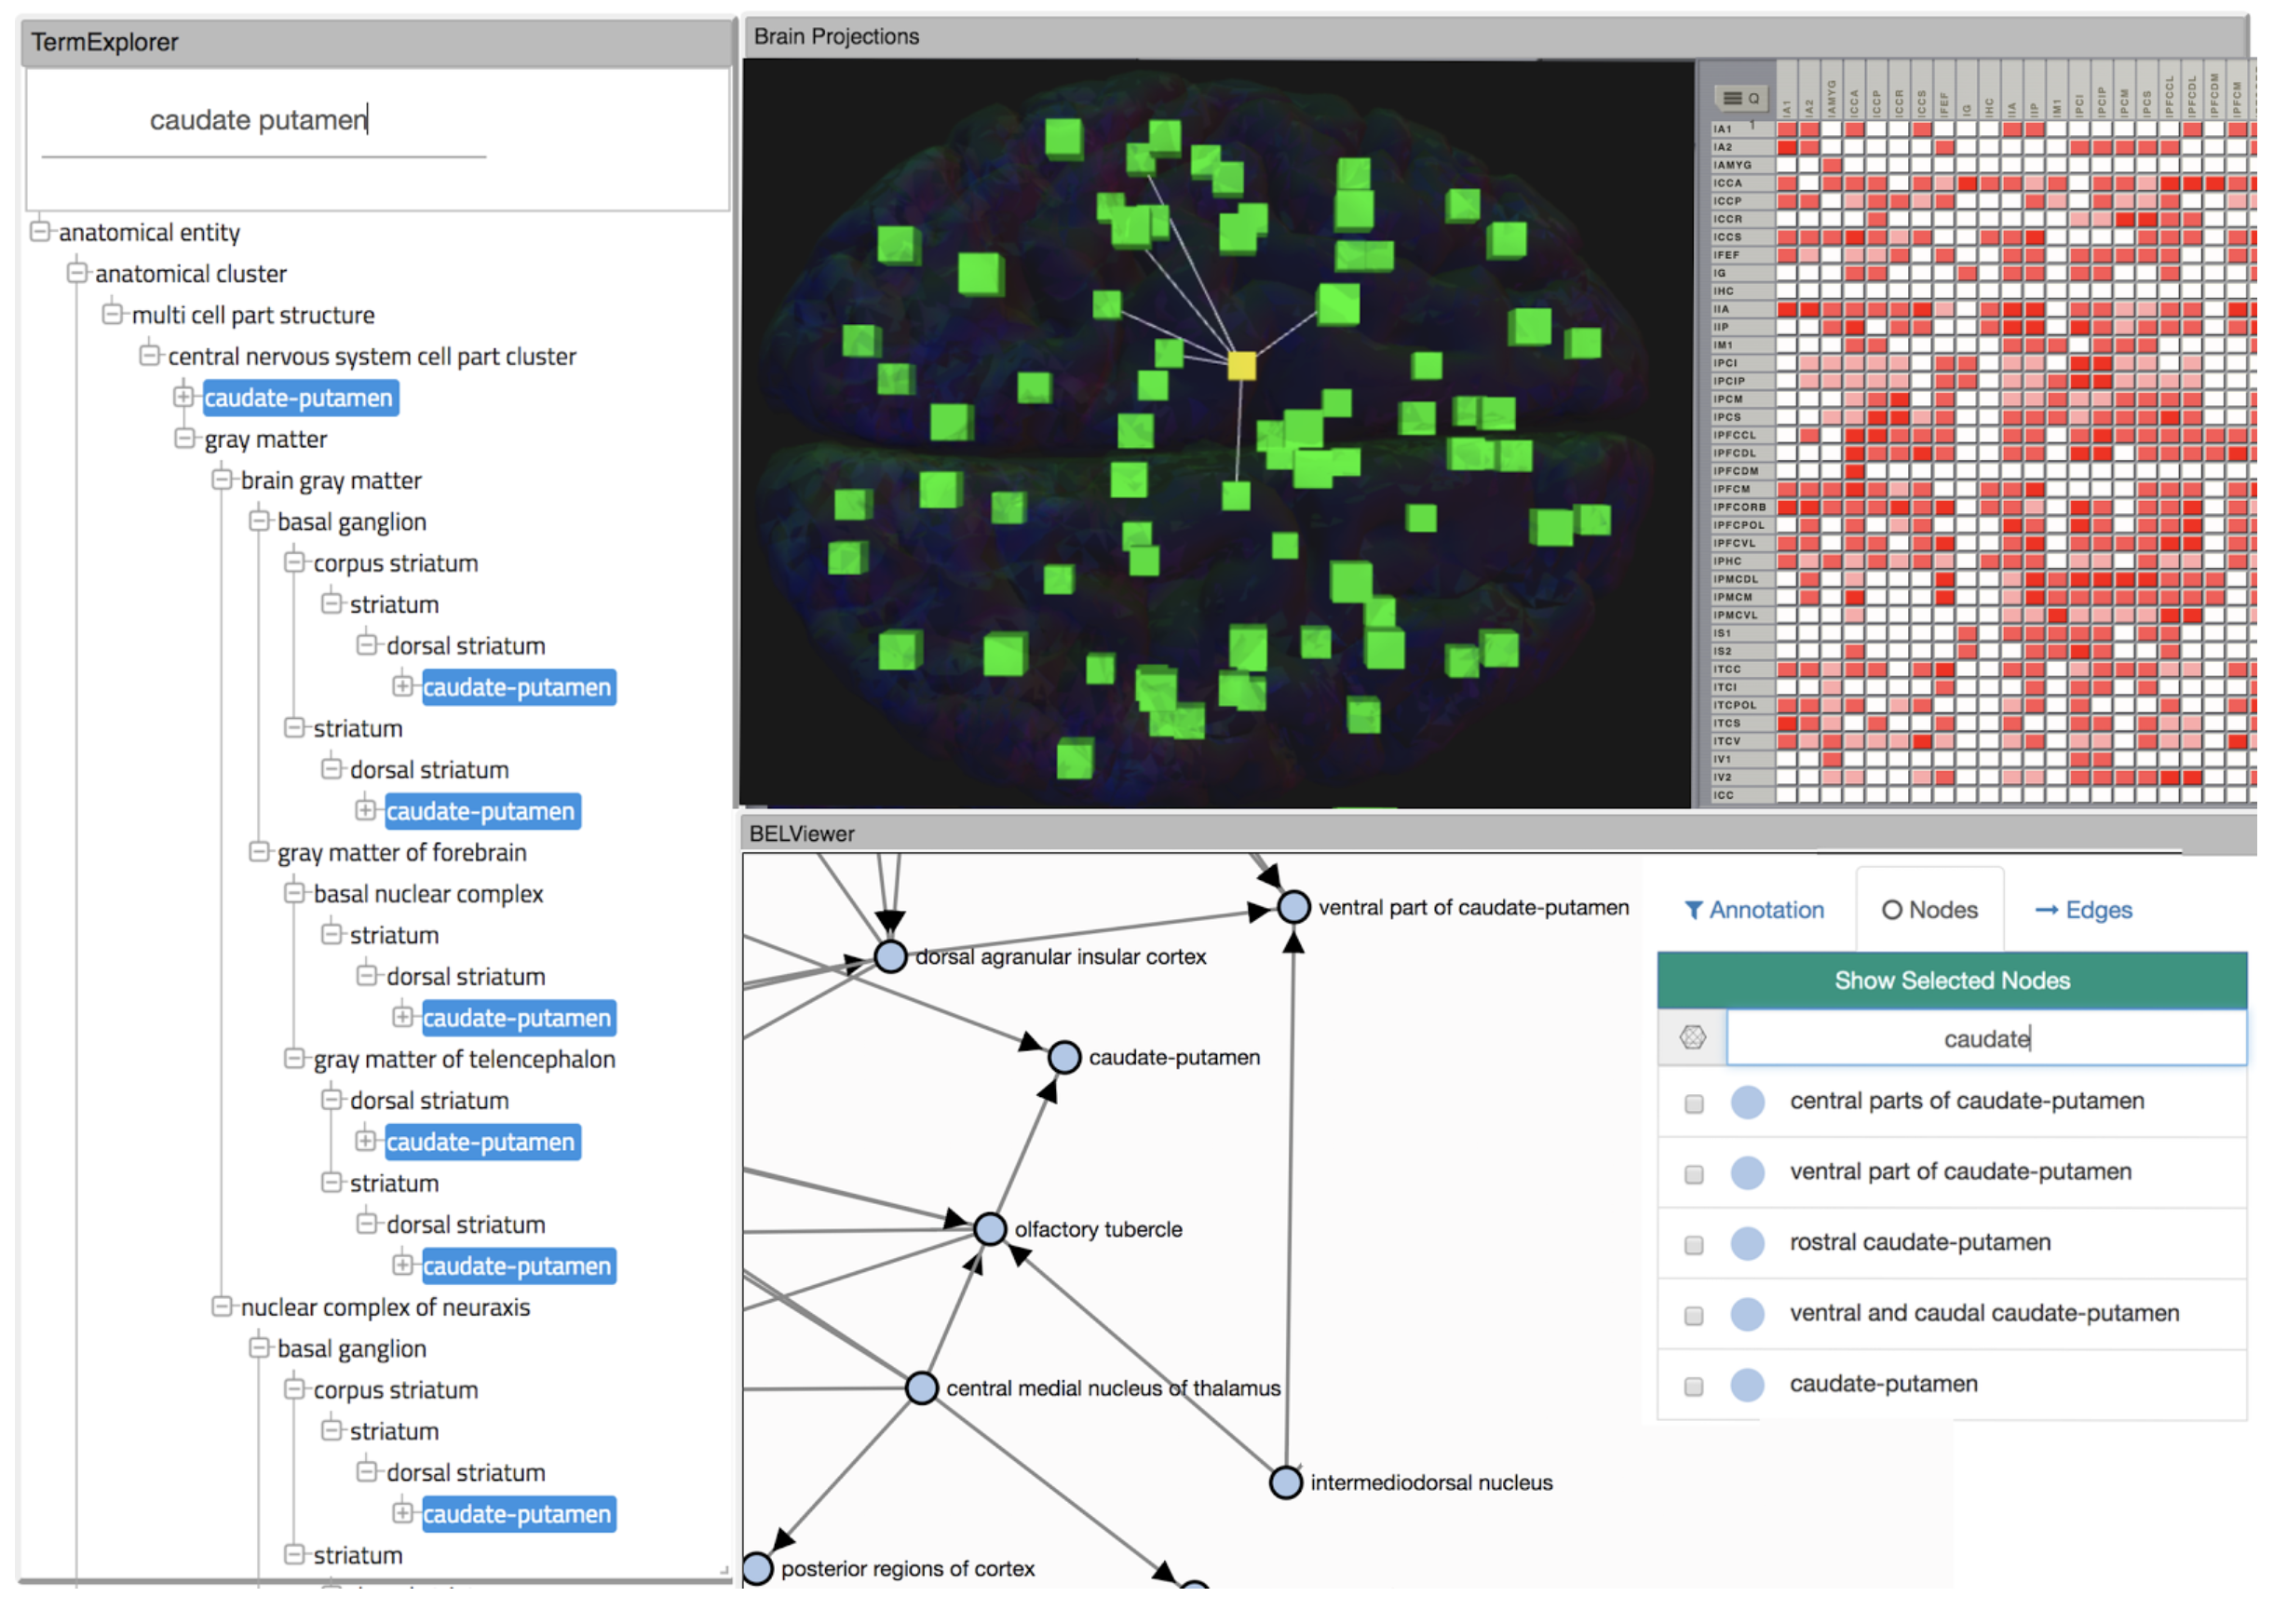
\includegraphics[width=160mm]{images/integration_tvb.png}}
\caption[PyBEL Integration with The Virtual Brain]{The PyBEL visualization system is linked to the tree browser from the Ontology Lookup Service \cite{Cote2006} and connectivity viewer from The Virtual Brain \cite{Leon2013} to allow for interactive exploration of the knowledge related to given brain regions as well as their undirected connectivity or directed projection information.}
\label{Fig:integration_tvb}
\end{figure}

\section{Remarks on Development}

\subsection{Software Stability}

This software was developed under a test-driven development cycle, where extensive unit tests were written to check the stability of the many functions that make up the five components of the software. The procedure for running these tests is encoded with the \verb|tox| build system that is automatically run by Travis \ac{CI} (https://travis-ci.org) upon each push of code to GitHub (https://github.com). The coverage of these tests are then assessed by CodeCov (https://codecov.io).

\subsection{Installation and Usability}

Travis CI also integrates with the "tags and releases" aspect of GitHub to enable automatic build of the code and distribution through PyPI (https://pypi.org), the main packaging system for Python. All relevant information for installation is bundled in the package, so it can be installed with zero configuration on any computer using \verb|pip install pybel| from any terminal, on any operating system, running any modern version of the Python programming language. Finally, the documentation for PyBEL is included in its repository and is automatically built with Sphinx (http://www.sphinx-doc.org) and uploaded to Read the Docs (https://readthedocs.org) upon each push of code to GitHub.

\section{Discussion}

\subsection{Extensibility of Syntax}

Even after its v2.0 update, the \ac{BEL} specification does not yet explicitly specify many concepts in molecular biology such as epigenetic information (e.g. methylation), which is a crucial part of modeling of complex diseases \cite{Irin2015}. The inevitability of language evolution prompted the development of the parser in modules so that new syntax could be proposed and implemented quickly. As a proof of concept, a syntax extension for gene modifications is included in the package by default.

\subsection{Extensibility of Resources}
Historically, \ac{BEL} namespace files have used a custom definition format; but the creation and maintenance of terminologies in the biological domain has tended towards the usage of \ac{OWL}. Furthermore, many namespaces such as dbSNP \cite{Sherry2001} are growing too large to enumerate during semantic integration and validation. The modular architecture of the PyBEL parser enables easy implementation of new definition file formats, external validation services, or even alternative schemes for definition statements to address these issues.

PyBEL introduces syntax for defining namespaces with a consistent pattern using a regular expression to overcome this issue. For these namespaces, semantic validation can be perform in post-processing against the underlying database. The dbSNP namespace can be defined with a syntax familiar to BEL annotation definitions with regular expressions as follows:

\verb|DEFINE NAMESPACE dbSNP AS PATTERN "rs[0-9]+"|

\subsection{Integration of Data}

While \ac{BEL} is often used to formalize knowledge curated from unstructured sources, PyBEL also accommodates the integration of knowledge from structured sources. Existing solutions for resolving equivalences across namespaces have relied on the creation and external hosting of extensive lookup tables. PyBEL could take inspiration from the \ac{OWL} format and enable equivalency information to be directly integrated in a network as edges. 

Again, the parser is extensible enough to implement dedicated syntax for equivalency similar to the standard syntax for gene orthology (\verb|orthologousTo|), protein complex component definitions (\verb|hasComponent|), and protein family membership (\verb|hasMember|). This is realized with the addition of the \verb|equivalentTo| relation, which can be reasoned over using network algorithms directly or collapsed for further use. For example, the fragments produced by amyloid cleavage can be represented in \ac{BEL} with either a protein and fragment combination, or referred directly by its entry in \ac{ChEBI} \cite{Hastings2013}. With the PyBEL extension, this can be written as:

\verb|p(HGNC:APP, frag(672_713)) equivalentTo \|

\verb|a(CHEBI:"amyloid-beta polypeptide 40")|

The hierarchical information encoded in ontologies can also be directly integrated. For example, integrating the \ac{ChEBI} Ontology could allow for reasoning over its multiple functional and structural hierarchies of chemical space. These entries can enable mechanistically-focused chemical repurposing strategies by identifying links between chemical inhibitors in disparate regions of a network \cite{Hastings2013}. 

\subsection{Inaccessible Formats}

Data locked away in other formats such as BioPax and SBML cannot be accessed by PyBEL currently. Development of knowledge assemblers, like \ac{INDRA} \cite{indra}, provide support for import of many formats. PyBEL will enable the import of \ac{BEL} documents much more quickly, and ultimately enable the export of \ac{SBML}. In the future, it would also be useful to develop additional interchange tools for \ac{BioPAX} to \ac{BEL}, but this is a large task that will be limited by the expressibility of each language and the difficult development of a two-way mapping.
There is ongoing work on integrating PyBEL and \ac{INDRA} to immediately make accessible the text mining results from REACH \cite{Valenzuela-Escarcega2015} and TRIPS \cite{Allen2008} as well as the prior knowledge sources assembled for the \ac{INDRA} workflow. Future work is planned to integrate the \ac{BELIEF} workflow \cite{Madan2016} as well.

\subsection{Comparison with Previous Software}

After describing PyBEL, Table 3 is used to make a direct feature comparison with the OpenBEL Framework and bel.rb. While the OpenBEL Framework has some features that are still in develop in the PyBEL ecosystem (see following section on Bio2BEL), PyBEL is the most feature complete and robust option.

\begin{table}
\centering
\caption[BEL Software Ecosystem Comparison]{A comparison of the available software for processing \ac{BEL}. *To the best of our ability, we were unable to install bel.rb using its documentation and unsuccessful in soliciting support through GitHub or OpenBEL's proposed channel of communication on Gitter (https://gitter.im/OpenBEL/chat)}
\label{tab:comparison}
\def\arraystretch{1.1}
\begin{tabular}{p{4cm} p{4cm} p{4cm} p{4cm}}
 & OpenBEL Framework & bel.rb & PyBEL \\
\hline
Programming Language & Java & Ruby & Python \\
Latest Official Release & 2015-06-11 & 1.1.2 - 2017-05-22 & 0.9.0 - 2017-09-19 \\
Installation & Not available on package manager such as brew or apt-get & \verb|gem install bel|* & \verb|pip install pybel| \\
BEL 2.0 Support & No & Experimental & Yes \\
Testing & Yes & Yes & Yes \\
Continuous Integration & No & Yes & Yes \\
Code Quality Testing & No & No & CodeCov and Code Climate \\
Documentation and Tutorials & No & Yes & Yes \\
Command Line Interface & Yes & Yes & Yes \\
Import & BEL Script & BEL Script, RDF & See Table 1 \\
Export & KAM Navigator & RDF & See Tables 1 and 2 \\
Visualization & KAM Navigator & None & See Figures 6-8 \\
Namespace Formats & BELNS & BELNS & BELNS and OWL \\
Compilation Process & Orthology, Named Complexes, Central Dogma & None & Central Dogma \\
Explicit Equivalence Handling & Yes & No & No \\
Extensible Parser & No & No & Yes \\
Programmatic API & No & No & Yes \\
Caching Mechanism & Yes & Yes & Yes \\
Internal DSL & No & Yes & No \\
Ongoing Development & No & No & Yes
\end{tabular}
\end{table}

\section{Conclusions}

\subsection{Applications in Re-curation}
The \ac{NeuroMMSig} knowledge assemblies for \ac{AD} and \ac{PD} had many syntactic, semantic, and biological errors. The PyBEL parser provides a much more useful error analysis than previous software and immediately enabled fixes for many of the syntactic and semantic errors. During this process, a preliminary version control process was implemented to track progress over time. With less than 200 commits and over a period of six months, 5327 of the 8030 errors in the Alzheimer's disease knowledge assembly and 465 of the 1171 errors in the Parkinson's disease knowledge assembly were fixed (Figure 12).

\begin{figure}
\captionsetup{format=plain}
\makebox[\textwidth]{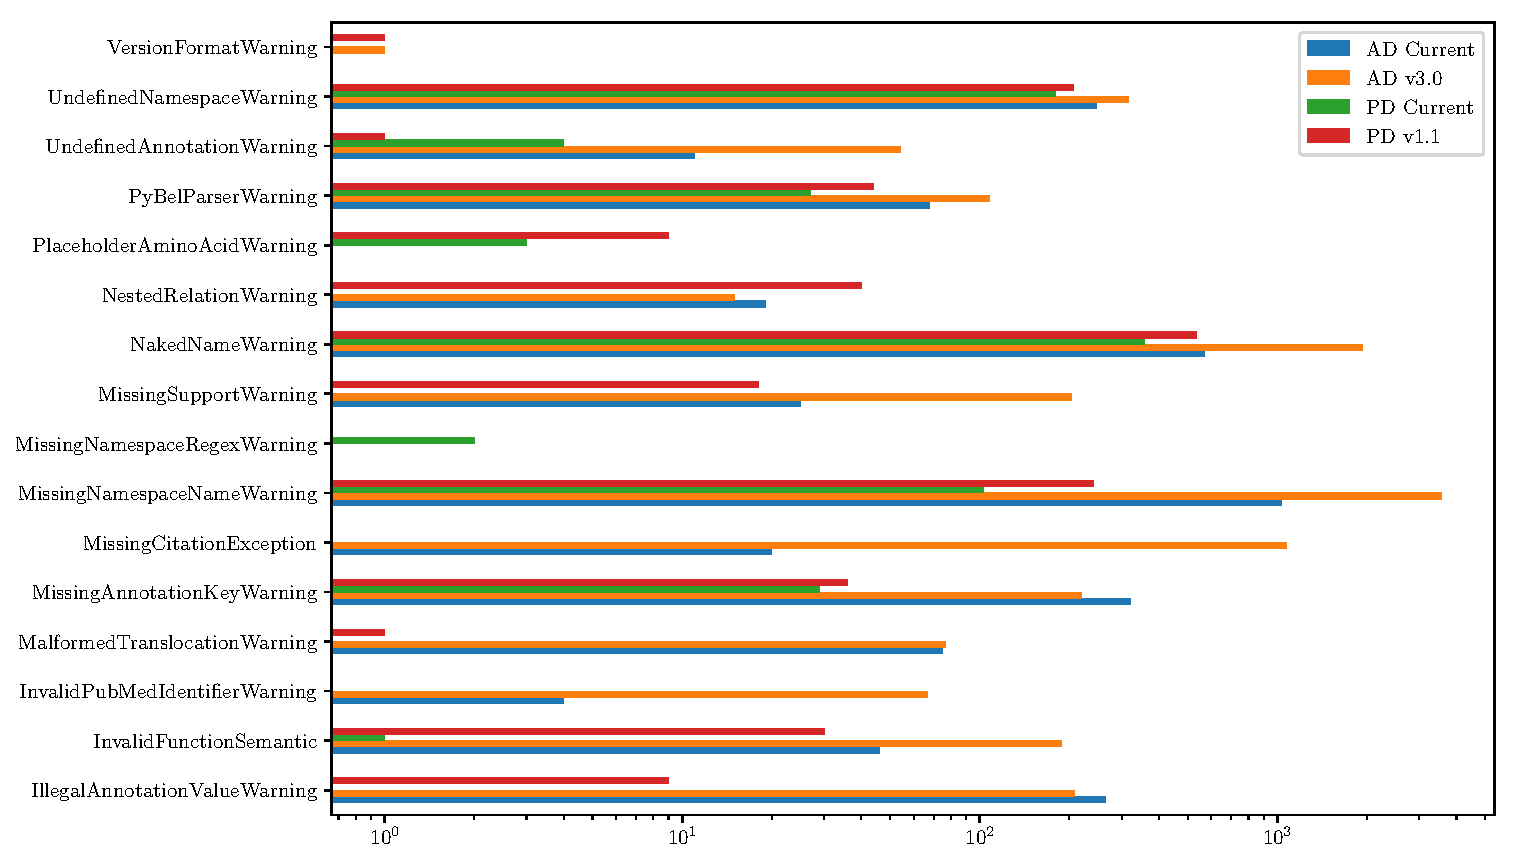
\includegraphics[width=160mm]{images/recuration_bars.pdf}}
\caption[NeuroMMSig Recuration Summary]{The re-curation efforts of the Alzheimer's disease and Parkinson's disease knowledge assemblies showed significant progress after the introduction of PyBEL.}
\label{Fig:recuration_summary}
\end{figure}

Biological problems are much more difficult to detect a priori, but later sections in this thesis describe how integrating data from external sources could allow for an assessment of the "biological grammar" underlying the knowledge assemblies. Future integration with \ac{INDRA} can provide the first steps in automatic analysis of biological correctness using its belief propagation algorithm for quantifying the reliability of statements  based on consensus across text mining and a-priori knowledge bases.

\subsection{Applications in Psychology and Psychiatry}

PyBEL has already been used to stretch the boundaries of manual curation. Projects dealing with anxiety and anhedonia have led to the curation of neuronal connectivity and projects. Other projects dealing with \ac{PTSD} and \ac{TBI} have led to a much larger focus on the curation of biological processes, phenotypes, and clinical measurements. The limited information on the molecular level combine with the focus on non-molecular clinical measurements in these domains motivates the need for integration of new a-priori knowledge bases to assist in the contextualization of new information, critical assessment of the completeness and correctness of new curated material, and new analytical techniques.

\subsection{Future Work}

Integrating chemical information systems like the Comparative Toxicogenomics Database \cite{Davis2017} could enable a previously envisioned chemoinformatics platform \cite{Emon2017} backed by the mechanistic knowledge encoded in \ac{BEL} networks. The extensibility of the network data container enables the integration of relations that are not explicitly defined by \ac{BEL}, such as weighted chemical similarities, for development of novel algorithms and analyses as well as enables the implementation of previously published algorithms for more general use. 


\chapter{Bio2BEL}
\label{ch:bio2bel}

\section{Background on Bio2RDF}

An outline was proposed as early as 1995 for integrating data in the biomedical domain that involved transforming data into a common model, aligning semantically related objects, integrating schemata, and federating data \cite{Davidson1995}. \ac{RDF} has the faculty to address these concerns, and were ultimately realized with the Bio2RDF project, in which multiple biological databases and knowledge bases were serialized to RDF for later integration \cite{Belleau2008}.

As stated before, the expressive power of RDF is counteracted by its lack of domain specificity. While it can be used as an interchange format, it still requires converters to formats for which analytical pipelines have already been developed. Furthermore, the suite of conversion scripts are written in PHP, which has very little traction in the bioinformatics community and therefore is difficult to integrate in pre-existing workflows. This section presents Bio2BEL: a project similar to Bio2RDF for the BEL community to directly the usage of the other tools presented in this thesis.

\section{Generation of Namespace Resources}

There are multiple granularities at which a terminology can be modeled. At the lowest is a vocabulary, in which each term is enumerated and described. Higher is a taxonomy, in which hierarchical relations are expressed. At the highest granularity is an ontology, which contains arbitrary and complex relations.

While it is not the primary goal of knowledge modeling, ontologies can also represent cross-references that connect multiple terminologies that describe the same entities. The most common model for representing ontologies is \ac{OWL} which most commonly uses \ac{RDF} as an interchange format, whose main goal is to provide a platform for semantic integration. This immediately provides ontologies with the facilities developed to support semantic data integration. This is very important in the biomedical domain as rapidly progressing technology frequently results in new experiments and new language for describing biological phenomena.

OWL, and a more domain-specific variant, \ac{OBO}, have been widely adopted by the biomedical domain to structure terminologies and enable semantic integration across knowledge and data sources \cite{Smith2007}. Multiple tools for storing, disseminating, and searching them have been including the Brenda Ontology Explorer \cite{brendaontologyexplorer}, BioPortal \cite{Whetzel2011}, OBO Foundry \cite{Smith2007}, and the EBI \ac{OLS} \cite{Cote2006}.

The semantics of the \ac{BEL} require entities to be identified with a name linked to a namespace. The original framework for handling \ac{BEL} Scripts also provided scripts for gathering different resources (vocabularies, taxonomies, and ontologies) in varying formats and assembling them in a specific namespace file format. One of the advantages of BEL over other systems biology modeling languages is its ability to model knowledge across modes and scales. As it is used to describe new phenotypes, such as the domain of psychiatry, new namespaces must be identified and formatted. Below, two approaches for building new namespaces are described.

\subsection{Direct Generation of Namespace Resources}

The OpenBEL Consortium distributed several scripts that included directives and parsers for acquiring data from multiple knowledge bases and databases and structuring them to BEL namespaces in a reproducible manner. Often, this is necessary to acquire identifiers that are not exported to a standard format like OWL or OBO. Additional scripts were written to improve the reliability of these generators and to convert new namespaces summarized in Table 4.

\begin{table}
\centering
\caption[Direct Namespace Generation]{Data sources for which reusable BEL namespace conversion scripts have been implemented}
\label{tab:direct_namespace_generation}
\def\arraystretch{1.2}
\begin{tabular}{p{5cm} p{10cm}}
Data Source & Description \\
\hline
FlyBase & Drosophila genes and gene products \\
HGNC & Human genes and gene products \\
HGNC Gene Families & Human gene families \\
InterPro & Protein families, domains, and binding sites \\
ChEBML & Experiments describing the effects of chemicals on proteins \\
MeSH Psychiatry and Psychology & A taxonomy of concepts from psychiatry and psychology  \\
dbSNP & \ac{SNP}s \\
miRBase & Premature and mature \ac{miRNA} sequences
\end{tabular}
\end{table}

\subsection{Indirect Generation of Namespace Resources}

BEL namespaces are not generally useful for curators or text-mining platforms to perform named entity recognition. The data sources from which BEL namespaces can be derived often have other rich information (synonyms, hierarchies, and cross-references) that could be structured into an ontology that is more generally useful. 

Some of the namespaces that were originally generated directly by the OpenBEL Framework are derived from ontologies. Since the development of this pipeline, the aforementioned services for hosting ontologies have gained popularity. The \ac{OLS} provides a programmatic \ac{API} from which the terms in a given ontology can be accessed. The source code for this service is available and can be hosted locally. 

The indirect approach uses data sources to build ontologies that can be hosted in \ac{OLS} then to use the \ac{OLS} \ac{API} to iterate over the terms' labels in order to easily convert any ontology to a BEL namespace with a reusable procedure. Already, namespaces in Table 5 have been generated from the publicly available \ac{OLS}. 

\begin{table}
\centering
\caption[OLS-Mediated Namespace Generation]{Ontologies deployed in the OLS from which BEL namespaces have been generated.}
\label{tab:indirect_namespace_generation}
\def\arraystretch{1.2}
\begin{tabular}{p{6cm} p{8cm}}
Ontology & Description \\
\hline
Human Phenotype Ontology & Clinical and phenotypic abnormalities \\
Uber Anatomy Ontology & Anatomical structures in animals
\end{tabular}
\end{table}

As a proof of concept, the data sources in Table 6 have been downloaded and converted to an ontology, deployed on a local \ac{OLS} instance, and converted indirectly to a BEL namespace.

\begin{table}
\centering
\caption[Indirect Namespace Generation]{Data sources from which ontologies have been generated, deployed, and used to generate BEL namespaces.}
\label{tab:indirect_ols_namespace_generation}
\def\arraystretch{1.5}
\begin{tabular}{p{6cm} p{8cm}}
Data Source & Description \\
\hline
\ac{UniProt} & Proteins \\
miRBase & Premature and mature \ac{miRNA} sequences
\end{tabular}
\end{table}

\subsection{Distribution of Namespace Resources}

Each method for downloading, parsing, and generating a namespace is stored as its own self-contained Python package. They share common methods for interacting with the \ac{OLS} in the \verb|ols-client| package. Finally, resources are uniformly deployed and distributed with Artifactory \cite{artifactory}. Common code for uploading to Artifactory is included in PyBEL-Tools. 

\subsection{Discussion Related to Resources}

Not all data sources are amenable to the indirect approach. Infamously, the \ac{MeSH} is a thorough data source that was not developed to accomplish the same goals as ontologies. Therefore, it is incredibly difficult task to map its data to an ontology. Furthermore, the implicit solution to semantic integration that relied on ontologies is not generally applicable. In these scenarios, it is not only necessary to generate a namespace, but also mappings. Previous efforts have relied on lookup tables, but like BEL namespaces, are not generally reusable.

Using ontologies to build namespaces implicitly solves the technical problem of mapping terms from one terminology to another, but this does not necessarily generally solve the biological problem. Mappings between identifiers may have different validity for different applications. While it is often convenient for biological literature to name proteins by their genes' names, this can create ambiguity for genes that produce multiple products in the cases of differential splicing and post-transcriptional modification. For example, in some simplistic domains, it is possible to map HGNC gene identifiers to \ac{UniProt} protein identifiers. However, when modeling complex phenotypes that rely on this mechanism, this mapping cannot be used.

\section{Knowledge Integration}

Knowledge can be represented as statements each consisting of a subject, predicate, and object. As knowledge is assembled, the object of one statement may be the subject of another. This process implicitly builds a knowledge network over which reasoning and inference may be performed. Two general purpose technical solutions for storing statements are relational databases and \ac{RDF}.

A relational database allows for similar statements, often ones with the same types of subjects, same types of objects, and same predicates, to be stored in tables. Each row represents one statement, where the subject and the object are assigned a column and additional columns can represent the metadata associated with the assertion of the statement. While their structure is explicitly, relational databases have the disadvantage of becoming large and complicated when representing many types of knowledge. As a result, many knowledge bases are disparate. Further, the management systems underlying relational databases are generally not amenable to federation.

One solution to this problem is to expose the database through \ac{API}s that can be queried from external services to enable federation of multiple relational databases. A popular solution is the \ac{REST} \ac{API}, but to integrate many data sources might require multiple queries, which can put a strain on technical systems. A newer solution is \ac{GraphQL}, which attempts to provide an abstraction layer between relational databases and \ac{REST} \ac{API}s to handle federation more efficiently.

An alternative medium to relational databases entirely is \ac{RDF}, in which all statements are explicitly stored as triplets of subject, predicate, and object in an alternative database management system called a triple-store. The underlying data can be exposed with a \ac{SPARQL} endpoint, which enables the statements to be queried. Further, it directly enables path queries to enable reasoning and inference. \ac{RDF} was developed to enable federation directly using \ac{SPARQL} endpoints from multiple data sources. It also does not need a well-defined schema in the same way a relational database does. This is both a blessing and a curse; new data can be added quickly, but the lack of structure makes it both technically and pedagogically difficult to make pointed queries.

\subsection{Utility of Biological Expression Language}
Because relational databases and \ac{RDF} are general solution for storing knowledge, they are unaware of the domain-specific needs of knowledge representation and storage in the biomedical domain. Among other modeling languages and formats for systems and networks biology, \ac{BEL} is an apt medium for storing structured knowledge extracted from the literature because it enables inference and reasoning over varying topologies of the resulting networks and also a serialization format for structured knowledge bases to enable integration in a domain-specific medium. It is a solution to overcoming the technical limits imposed by RDF on representing relation metadata and the technical limits imposed by relational databases in constructing and querying networks.

BEL is commonly used for manual curation in a specific disease area. Integrating prior knowledge sources to these networks provides context not only to assist the curator in their understanding of the biological knowledge surrounding their curation, but also allows for automatic enrichment, improved reasoning, and a further step towards building a support system for data interpretation. 

Among the most easily integrable structured knowledge formats in BEL are taxonomies, ontologies, and networks. Taxonomies and ontologies directly provide the facility for reasoning and inferences of new knowledge. Networks, such as bipartite \ac{SNP}-disease, chemical-gene, or gene-pathway networks, can be directly integrated in \ac{BEL}. Even networks created by statistical calculations can be added to \ac{BEL} networks to investigate their explanatory power. For example, the \ac{eSNPO} provides statistical associations between \ac{SNP}s and \ac{GO} biological processes. While these don't have mechanistic support, they can provide additional insight and allow for more informed hypothesis triage in network analysis. Here, two approaches for serializing structured knowledge sources to \ac{BEL} are described.

\subsection{Direct Generation of Knowledge Resources}

While structured, the formats in which knowledge is stored varies by domain. For example, ChEBML \cite{Gaulton2012} is distributed as a relational database, while BKMS-react \cite{Schomburg2017} uses a table with specifically formatted entries to describe reactions. For each source in Table 7, a reusable Python library that downloads, structures, queries, and serializes \ac{BEL} was developed.

\begin{table}
\centering
\caption[Direct Knowledge Resource Generation]{Knowledge bases for which reproducible BEL serialization procedures were implemented.}
\label{tab:direct_knowledge_generation}
\def\arraystretch{1.5}
\begin{tabular}{p{25mm} p{20mm} p{45mm}}
Knowledge Source & Type & Description \\
\hline
ChEMBL & Relational Database & Chemical inhibition and binding of enzymes \\
HGNC Orthologies & Tabular & Gene orthology mappings between human, rat, and mouse \\
BKMS-react & Tabular & Biochemical reactions and catalytic enzymes \\
\ac{eSNPO} & Tabular & Relations between \ac{SNP}s and biological processes
\end{tabular}
\end{table}

\subsection{Indirect Generation of Knowledge Resources}

Serializing knowledge to \ac{BEL} is not generally useful outside of the domain of tools directed towards \ac{BEL} networks.  The knowledge bases from which \ac{BEL} can be derived often have other rich information that is not appropriate for \ac{BEL} that could be structured in other knowledge representation models such as \ac{OWL}. For these cases, the parser and serializer were separated in order to build an intermediate relational database. These have the added benefit of being queryable through \ac{SQL} or exposed with RESTful \ac{API}s for large data sets across networks. Finally, these database schemes have the additional benefit of providing a formalism for the knowledge before serializing it to BEL. As a proof of concept, packages have been developed for the parsing, database storage, and BEL serialization for sources listed in Table 8.

\begin{table}
\centering
\caption[Indirect Knowledge Resource Generation]{Knowledge bases for which an intermediate solution for downloading, parsing, and modeling data were used to facilitate the development of reproducible BEL serialization procedures.}
\label{tab:indirect_knowledge_generation}
\def\arraystretch{1.5}
\begin{tabular}{p{25mm} p{20mm} p{45mm}}
Knowledge Source & Type & Description \\
\hline
Comparative Toxicogenomics Database & \ac{XML} & Relations between chemicals, genes, pathways, and phenotypes \\
InterPro & Hierarchy & Protein Family Hierarchies \\
HGNC Gene Families & Tabular & Gene Family Hierarchies
\end{tabular}
\end{table}

\subsection{Discussion Related to Knowledge Resources}

Many more knowledge bases and data sources exist that could be integrated with \ac{BEL}. For example, \ac{miRNA}-Target interactions stored in mirTarBase \cite{Chou2016} could provide insight to the complex regulation patterns that applies to complex diseases. Other sources of knowledge could be extracted from data-mining pipelines, such as linkage disequilibrium block analysis, gene co-expression analysis, and perturbagen-based differential gene expression analyses to provide additional support to elucidate mechanistic insight from increasingly complicated and large knowledge assemblies.


\chapter{PyBEL Tools}
\label{ch:pybel_tools}

The following section describes a subset of the functions and workflows that have been developed to assess, enrich, and analyze knowledge assemblies parsed by PyBEL. All code is made available as open source and stored in the PyBEL Tools repository (https://github.com/pybel/pybel-tools) on GitHub. Like PyBEL, it is thoroughly documented as to allow for the community to build upon it.

\section{Critical Assessment of Networks}
Before knowledge assemblies can be used to help interpret data, their validity and robustness must first be quantified. While many dimensions can be explored during this quantification, this section places focus on the identification of biological network motifs that indicate inconsistencies in the knowledge assembly. Network motifs have been studied in the context of transcriptional and phosphorylation networks \cite{Alon2007} and already provide insight to the biological activity. As knowledge networks add the heterogeneity of edges including correlative relationships, many new motifs must be identified and their effects inferred. This section presents the first portions of a taxonomy for network motifs in knowledge assemblies, interpret their effects, and use them assess the \ac{NeuroMMSig} knowledge base.

\subsection{A Taxonomy of Knowledge Assembly Motifs}

The first and most simple motif is a contradictory pair. These occur when there exist multiple edges between a given source and target that have conflicting relations, such as increases vs. decreases. However, contradictory pairs are not canonically invalid. They may arise from the effects of the biological context under which different relations were observed. These cases must be carefully considered.

There are many aspects that can be considered to resolve conflicts that cannot be explained by different biological scenarios. First, the date of publication can be considered. The most recent publication is most likely to have made use of other knowledge available to researchers, and be more right. Alternatively, if many publications were made with conflicting views in a short amount of time, the impact factor of the corresponding citations' journals can be considered.  

While there exists a single motif for identifying contradictory pairs, multiple motifs comprise the set of contradictory triplets. The algorithms that identify these triangles within a network come from a deep graph theoretic background to identify logically inconsistent relations. Because BEL knowledge graphs contain both causal and correlative relations, they can be analyzed jointly. The most simple is a mutually unstable triplet, which occurs when entities A, B, and C all negatively correlate with each other. Similarly, separately unstable triplets occur when A positively correlates with both B and C, but B and C are negatively correlated. Three more triple types are identified where a mix of  correlative and causal relations do not match: increase mismatch triplets, decrease mismatch triplets, and jens triplets.

Alternatively, stability analysis can be conducted to identify elements that are likely to be regulated by other parts of a system. These elements are particularly interesting because of the high impact that any given edge could have that connects to it. There are two types of unstable pairs: chaotic pairs, where A and B both increase each other and dampened pairs, where A and B both decrease each other. The same logic extends to chaotic triplets and dampened triplets. Interestingly, analyses of many knowledge assemblies seldom identified dampened triplets; possibly indicating their biological novelty. Chaotic and dampened cycles of length 4 and above are not identified, because the average number of possible connections at those lengths makes qualitative biological interpretation prohibitively difficult. 

Table 9 presents statistics over the occurrence of various network motifs in the three knowledge assemblies produced during the AETIONOMY project. While each case, such as mutually unstable triples, might be interesting, this provides direct insight into the large amount of effort necessary to investigate each unstable motif and motivates the further development of automated approaches for quantifying the robustness of a given knowledge assembly.

\begin{table}
\centering
\caption[Stability Analysis of NeuroMMSig]{Stability analysis statistics over the AETIONOMY knowledge assemblies for Alzheimer's disease, Parkinson's Disease, and Epilepsy. The ratios suggest that the relative counts of each network motif are not similarly correlated with network size or density. }
\label{tab:stability}
\def\arraystretch{1.5}
\begin{tabular}{p{55mm} p{25mm} p{25mm} p{25mm}}
 & \ac{AD} Knowledge Assembly v4.0.3 & Epilepsy Knowledge Assembly v1.1.2 & \ac{PD} Knowledge Assembly v1.1.1 \\
Chaotic Pairs & 56 & 12 & 16 \\
Chaotic Triples & 115 & 27 & 11 \\
Contradictory Pairs & 68 & 18 & 26 \\
Dampened Pairs & 7 & 2 & 4 \\
Dampened Triples & 1 & 0 & 2 \\
Decrease Mismatch Triples & 20 & 0 & 6 \\
Increase Mismatch Triples & 51 & 4 & 20 \\
Jens Unstable Triples & 657 & 153 & 85 \\
Mutually Unstable Triples & 2 & 0 & 7 \\
Regulatory Pairs & 19 & 9 & 15 \\
Separately Unstable Triples & 16 & 0 & 16
\end{tabular}
\end{table}

\subsection{Discussion}

As data integration projects like Bio2BEL make more data accessible during analysis, further plausibility and stability checks can be performed. One would be to integrate the data from \ac{UniProt} for each function and traverse the Gene Ontology molecular function annotations to identify properly annotated activities and flag improperly annotated ones to be either proposed as new, or fixed. Another example would be to check that protein and gene modifications are annotated properly using \ac{UniProt} and dbSNP, respectively. Adding additional checks using prior knowledge makes \ac{BEL} curation much more accessible to curators with less biological knowledge and also text mining systems that currently have less biological intuition.

\section{Survey of Algorithms}

Algorithms for analyzing pathways and networks can be categorized into three main categories: \ac{ORA}, \ac{FCS}, and \ac{PT} \cite{Khatri2012}. Over-representation analysis often focuses on the number of differentially expressed genes present or absent in a gene set compared to chance, while functional class scoring is less susceptible to large effects and considers the aggregate of groups of small effects. Pathway topology finally considers the biological relations between members of the pathway during analysis.

Furthermore, there is a distinction between methods that rely on the assumption that protein activities are correlated with their corresponding \ac{mRNA}s' expression changes (forward reasoning) versus the effect that upstream controllers of \ac{mRNA} expression have (backwards reasoning) \cite{Martin2014}

These algorithms have been developed for a wide variety of applications, data formats, and graph types. While many are heterogeneous, below are the most notable algorithms specific to networks from knowledge assemblies encoded in \ac{BEL}.

\subsection{Reverse Causal Reasoning}

Reverse causal reasoning (\ac{RCR}) is an approach to identify the upstream controllers of biological patterns measured in an experiment; often differential gene expression experiments between healthy and diseased patients. First, large knowledge assemblies are dissected into smaller hypothesis networks with one upstream node with multiple outgoing causal relations to target nodes represented by the experimental data set. Each hypothesis network is scored by its concordance between the observed up- and down-regulations of targets nodes to the sign of the causal relation and by its richness, or the explanatory power of the hypothesis network \cite{Catlett2013}. An example hypothesis network is shown in Figure 13.

\begin{figure}
\captionsetup{format=plain}
\makebox[\textwidth]{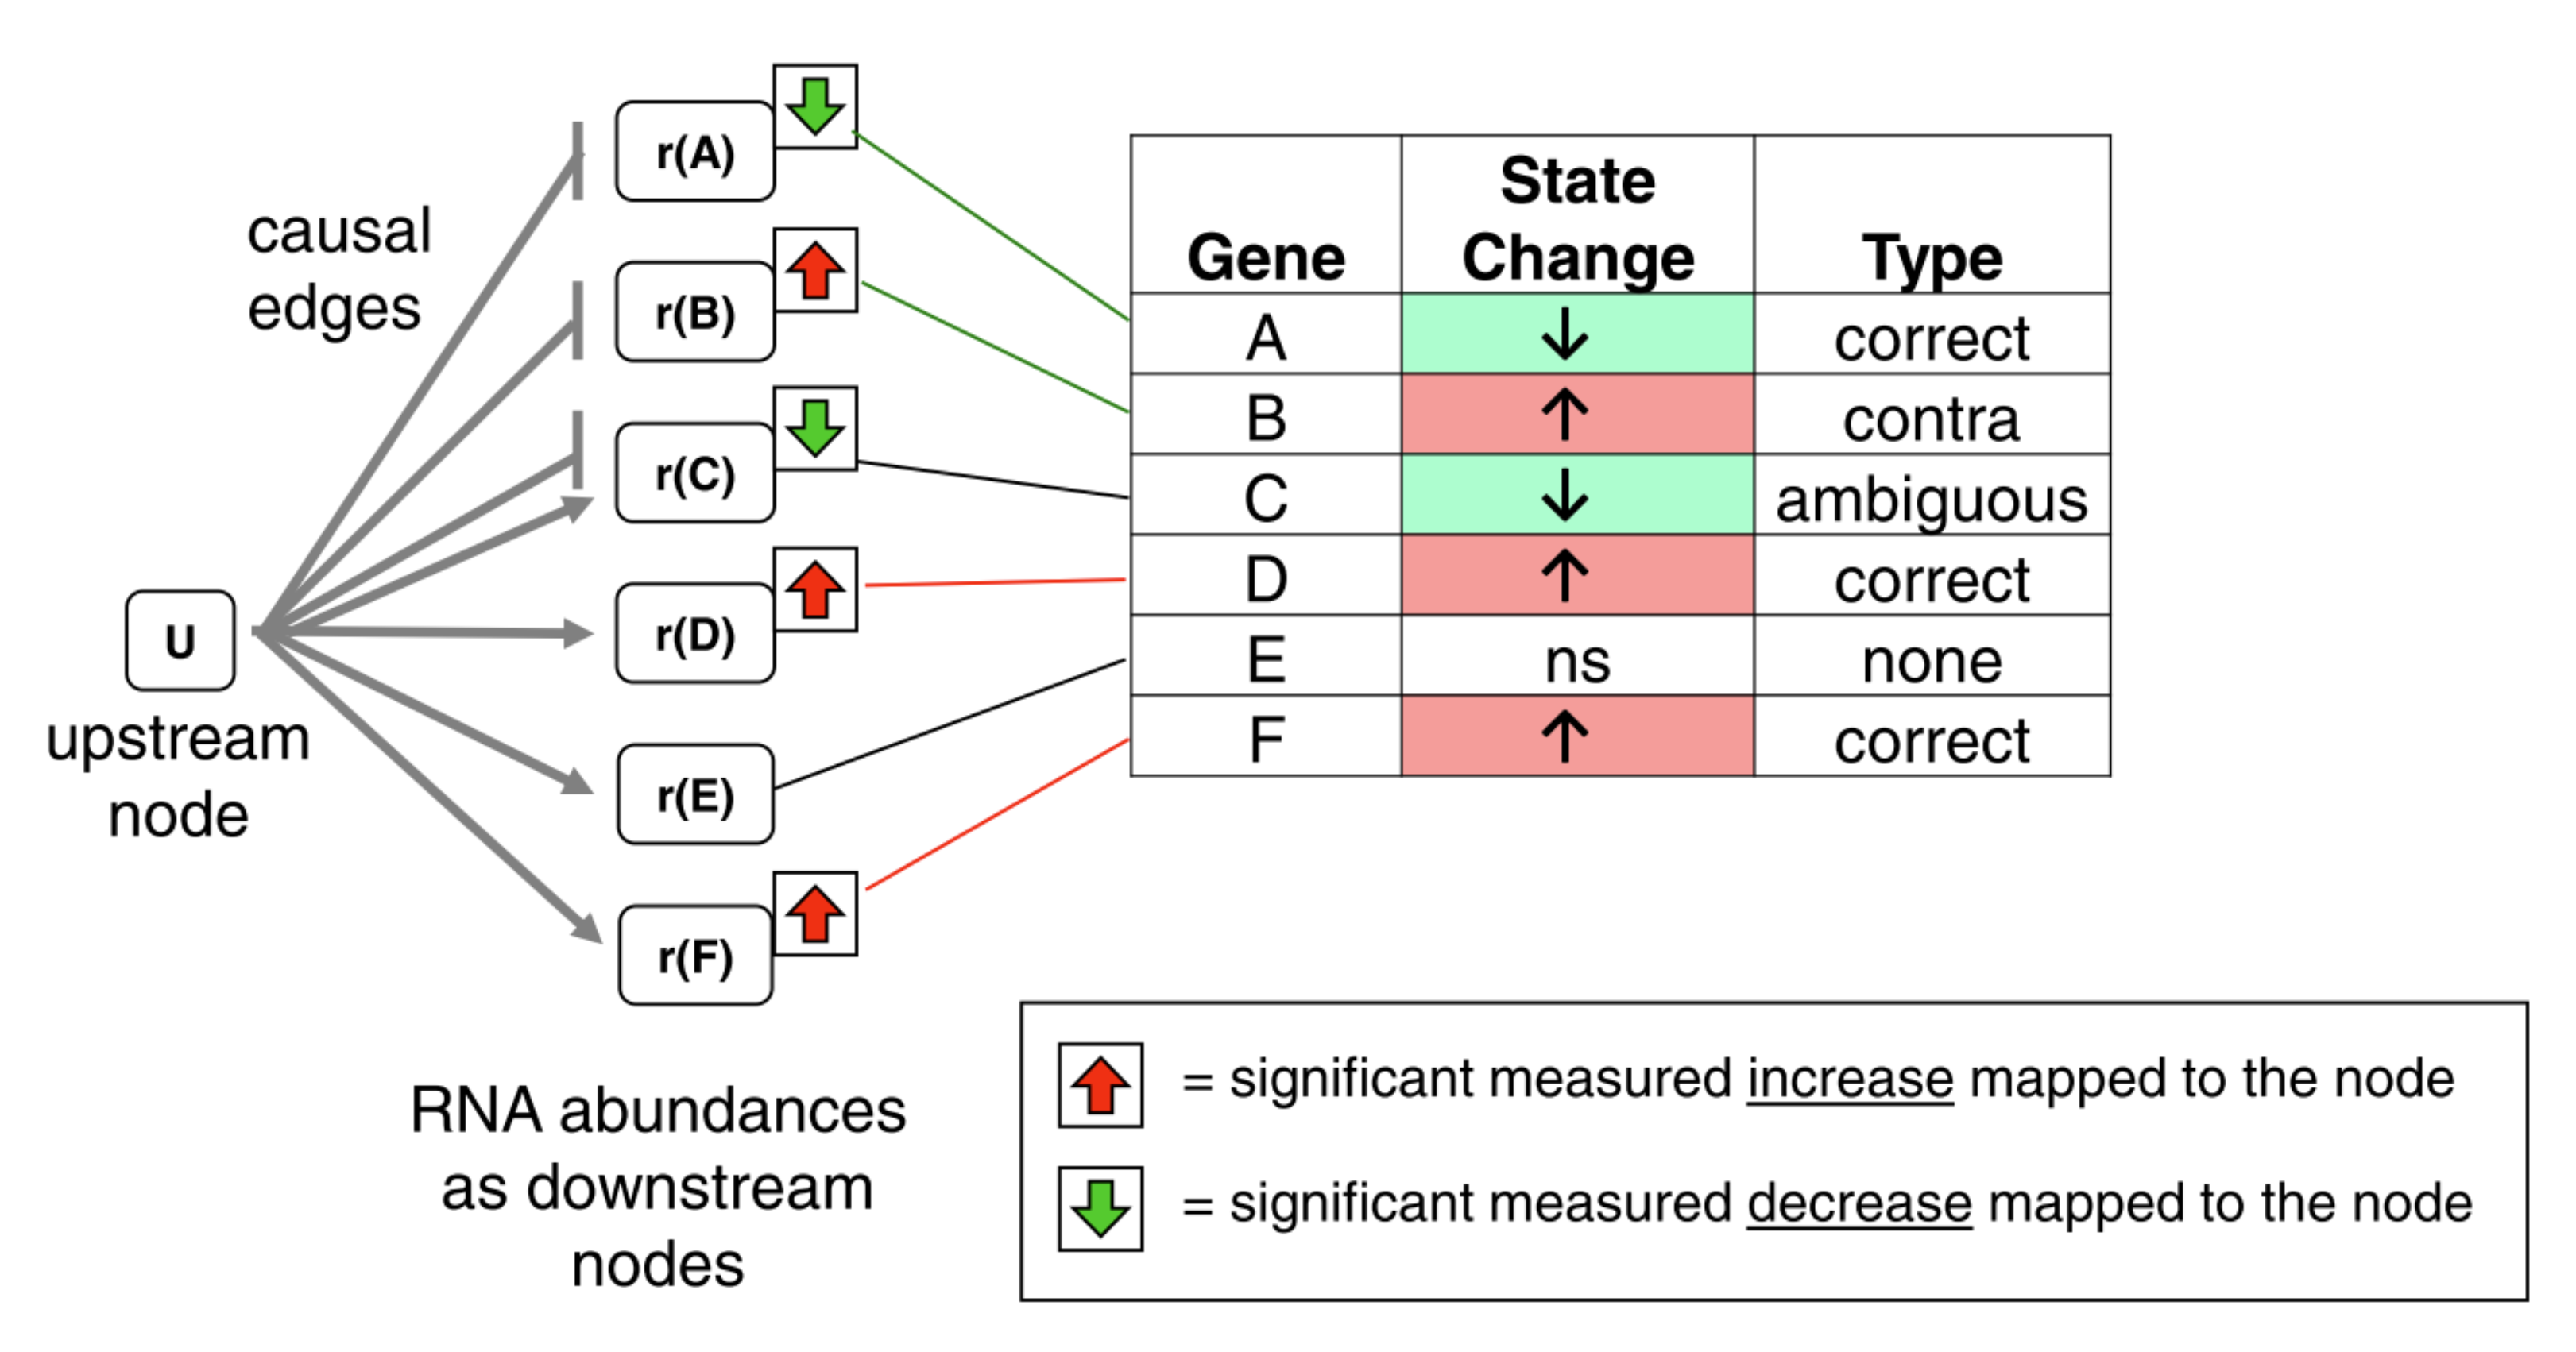
\includegraphics[width=160mm]{images/rcr_schematic.png}}
\caption[A Schematic Diagram of \ac{RCR}]{An example hypothesis network. Target nodes are counted as correct if they have a decreasing relationship and down-regulation, or an increasing relationship and up-regulation. Target nodes with multiple conflicting relationships are marked as ambiguous. Finally, target nodes are counted as incorrect if they have a mismatch between an increasing relationship and down-regulation, or a decreasing relationship and up-regulation. Adapted from \cite{Catlett2013}.}
\label{Fig:rcr_schematic}
\end{figure}

\subsection{Network Perturbation Amplitude}

While \ac{RCR} gives preliminary insights to significant biological controllers, it mostly ignores the topology of signaling, regulatory, and other causal networks that can be represented in knowledge assemblies (Figure 14). The \ac{NPA} measures the aggregated effect explained by the controller layer with reference to a given node with respect to their downstream nodes. Two complementary statistics for the effect of permutations of the upstream layer and downstream layer allow for further insight to the validity of \ac{NPA}s as a hypothesis generation mechanism \cite{Martin2014}.

\begin{figure}
\captionsetup{format=plain}
\makebox[\textwidth]{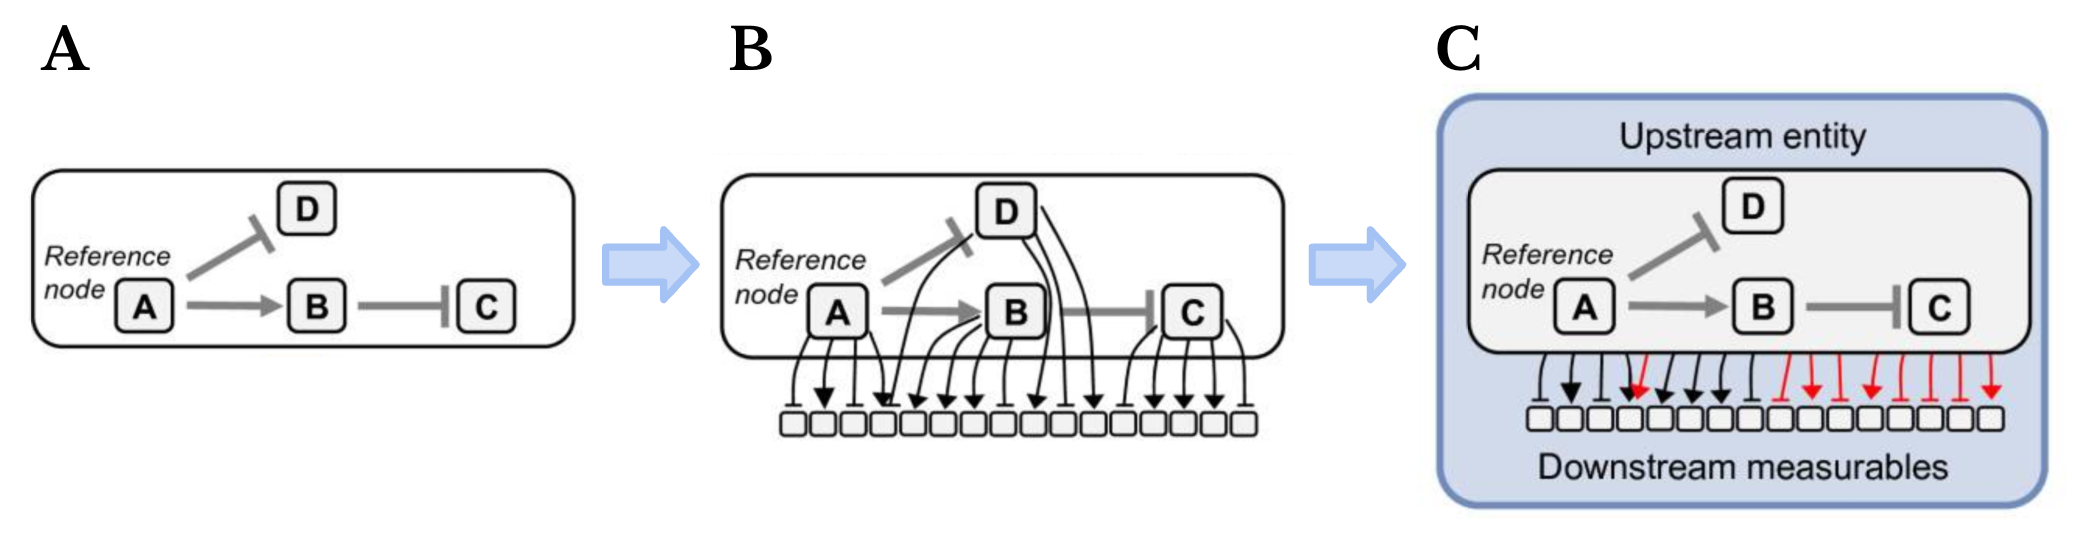
\includegraphics[width=160mm]{images/npa_schematic.png}}
\caption[Hypothesis Network Generation for Network Perturbation Amplitude]{Creation of hypothesis networks that accounts for the topology and interactions of  upstream controller layer with respect to a reference node A), their individual effects on the downstream layer B) and their combine effect C). Adapted from \cite{Martin2012}.}
\label{Fig:npa_schematic}
\end{figure}

\subsection{Sampling of Spanning Trees}

While \ac{NPA} enables more informed analyses than \ac{RCR}, its mathematical basis limits the topologies of knowledge networks that can be used to those with causal consistency. In these networks, all paths from one node to another result in the same aggregated effect of increases and decreases. An additional approach in Figure 15 for \ac{SST} with random walkers eliminates inconsistencies and can be aggregated over multiple trials to assign \ac{NPA} scores to networks that were otherwise inconsistent \cite{Vasilyev2014}. 

\begin{figure}
\captionsetup{format=plain}
\makebox[\textwidth]{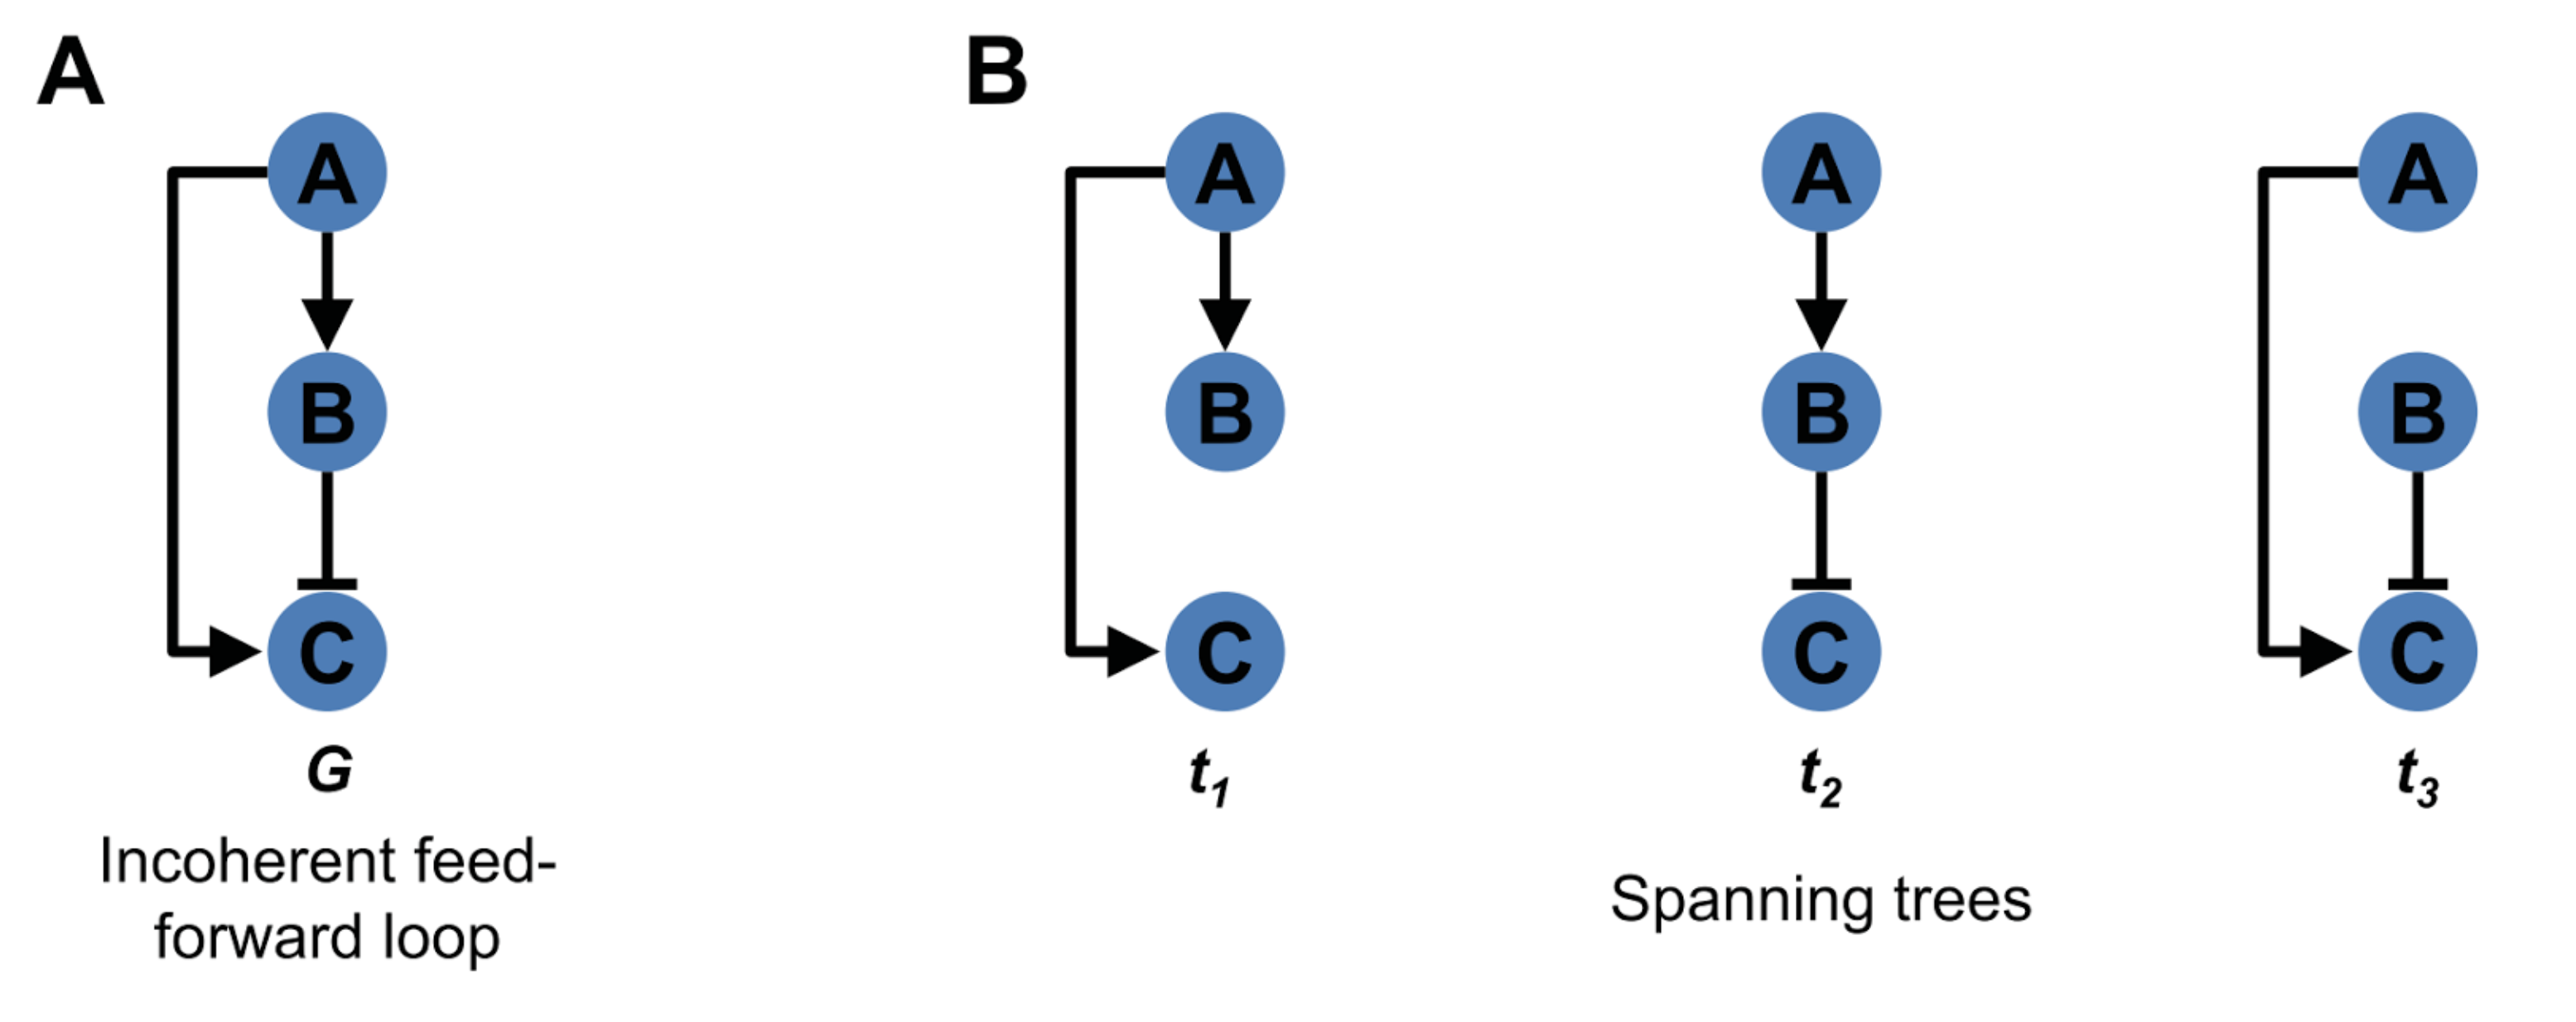
\includegraphics[width=160mm]{images/sst_example.png}}
\caption[Decomposition of Spanning Trees]{An example decomposition of a small causally inconsistent network A) to its spanning trees B)\cite{Vasilyev2014}.}
\label{Fig:sst_schematic}
\end{figure}

\subsection{Unsolved Issues}

While these algorithms already provide significant insight, they still have unresolved issues. For example: they require prior definitions of the upstream controller layer subnetworks; they do not address other exotic network motifs such as contradictions; and they do not take advantage of the vast assembly of correlative relationships. Further, there is generally a low coverage of nodes present in data sets within knowledge assemblies.

As mentioned before, these algorithms were developed for domains (oncology, immunology, etc.) that are rich in molecular data and mechanistic knowledge. For disease areas such as neurodegenerative diseases, molecular data (e.g., microarray, \ac{RNA}-seq) are not often available for the most applicable cells or tissues because of the practical difficulty of acquiring samples. It follows that context-specific knowledge is also much more sparse; and inference from other contexts (such as animal models) is much less reliable.

While backwards reasoning overcomes the issues with interpretation that are posed by forwards reasoning, the insufficient knowledge and data in neurodegenerative diseases makes this revelation much less useful. 

The experimental data available in for this field and other complex diseases are often multi-modal and multi-scale, prompting the development of new methods. Many of these experiments can only be connected to current knowledge assembles through correlative relationships, such as the associations between single nucleotide polymorphisms (\ac{SNP}s) and clinical phenotypes such as neuroimaging and gene expression. 

\section{A Priori Network Augmentation}

This section first describes pipelines that make biological knowledge assemblies more usable that rely on prior knowledge from the biomedical domain. Before developing analytical algorithms, it is first necessary to consider pipelines that improve the features of currently existing networks. After, an algorithm for generating upper layer controller networks is proposed and an alternative heat-diffusion method that is better able to accommodate heterogeneous experimental data. 

\subsection{Connecting Disconnected Components}

The GABA Subgraph in the Alzheimer's disease knowledge assembly has five disconnected components. While these can be inspected manually and the gaps can be filled, this becomes a daunting task for the set of 128 subgraphs in NeuroMMSig. PyBEL can be used to build queries that automatically expand and enrich graphs in order to create an environment in which disparate knowledge can be assembled to elucidate mechanistic understanding. Below, a procedure for filling in the holes in a subgraph is outlined. 

First, the central dogma is inferred. This ensures the existence of the corresponding RNA for proteins, and the corresponding genes for each \ac{RNA} and \ac{miRNA}. Doing so already connects the subgraph containing the relations describing how estradiol affects the expression of GABRA4 and GABR3 \ac{mRNA} \cite{Noriega2010} to another component that describes the functional impact of their translated proteins on other proteins and biological processes. After this process, four components remain.

Next, unqualified edges are enriched. This method reasons over nodes for which assertions can automatically be presumed. Relationships describing the different types of variations on genes and proteins (epigenetics, mutations, and post-translational modifications) are able to connect the GRIN2B node that is important in one large component to the phosphorylated GRIN2B node in another network. Because \ac{BEL} represents knowledge assemblies and not necessarily mechanistic models, these pieces of information can come from multiple curators without mutual knowledge. After this process, two components remain.

Of the two components, there is one large component and one small component, consisting only of cAMP catabolic process and GABBR2. While they are not yet automatic, further knowledge-based approaches can be used to connect GABBR2 to GABBR1 in the large component using resources like \ac{HGNC} Gene Families \cite{Gray2015}, InterPro \cite{Finn2017}, or PFAM \cite{Finn2016}. This is valuable because hierarchical knowledge sources like these can be used to reason over the network, like using the knowledge that GABBR2 decreases the cAMP catabolic process  \cite{Massone2011} to assert that GABBR1, the other member of the GPCR family 3, GABA-B receptor (IPR001828), shares the same activity. While this knowledge does not exist in the assembly, literature search also notes several connections between GABBR1 and cAMP signalling \cite{Frere2004,Palmer2005}.

\subsection{Subgraph Membership Inference}

While connecting components is important, it would also be useful to identify and add edges that should belong to the GABA subgraph but do not already. The first method would be to identify and edges occurring between nodes in the subgraph that are not already present, and add them. Next, this procedure can be continued to identify nodes that have edges to multiple nodes already in the subgraph. To reduce false positives, nodes added this way must both be the target of a causal relationship from a node in the subgraph and also have a causal effect on another node in the subgraph.

Finally, to improve viewability, two additional filters are provided. First, a filter for pathologies is used to remove them. This is useful since most pathologies are "super nodes" in knowledge assemblies and have numerous and often uninformative correlative relationships. Next, the central dogma is collapsed such that genes, \ac{RNA}s, and proteins are all shown as one node. While this limits the mechanistic explanatory power of a visualization, it removes a significant amount of visual clutter. 

\subsection{Pipeline Building}

It may be reasonable for viewing purpose to additionally collapse nodes representing modifications to their reference node as well. The submodule \\ 
\verb|pybel-tools.mutation| contains large library of functions that can be chained together either manually, or with a pipeline builder to promote reusability by allowing uses to save their workflows and reuse them. 

\section{Data Driven Analysis}

\subsection{Unbiased Candidate Mechanism Generation}

There are many terms used to describe portions of biological networks including pathways, mechanisms, subgraphs. They all comprise of individual interactions that accumulate to a more complex function. Often, an interaction may be part of multiple of these features. Knowledge bases like \ac{KEGG}, Reactome, and WikiPathways organize interactions into pathways; but they all suffer from bias in the literature and from the knowledge of their curators. This section presents an algorithm for generating unbiased candidate mechanisms from a given knowledge assembly. The method is then compared to the NeuroMMSig knowledge base to identify its ability to reproduce dogmatic subgraphs and identify areas of the underlying knowledge assemblies that have yet to be annotated.

In biomedical knowledge assembly across scales, biological processes represent entire subnetworks of causal interactions through both time and space. The \ac{NeuroMMSig} knowledge base captures associative, correlative,  and causal relationships between genes and gene products and biological processes directly in BEL. Because biological processes implicitly represent functional subnetworks, they are an appealing starting point for automatically unbiased generating candidate mechanisms to be used by other algorithms. 

The upstream controllers of biological processes provide direct insight to their functional impacts across scales. Therefore, the simple algorithm for generating candidate mechanisms that are unbiased by the dogmatic  takes the causally upstream controllers of a biological process, their upstream controllers, and all internal causal edges between them as a candidate mechanism. This method is thresholded at an expansion of two neighborhoods, but could easily be modified to choose larger or smaller lengths.

\subsection{Comparison to NeuroMMSig Knowledge Base}

This method was applied to the NeuroMMSig Alzheimer's disease knowledge assembly for each biological process. After, the resulting candidate mechanisms are compared to the NeuroMMSig subgraphs. First, the landscape of biological process membership in each subgraph is summarized with Figure 16. 

\begin{figure}
\captionsetup{format=plain}
\makebox[\textwidth]{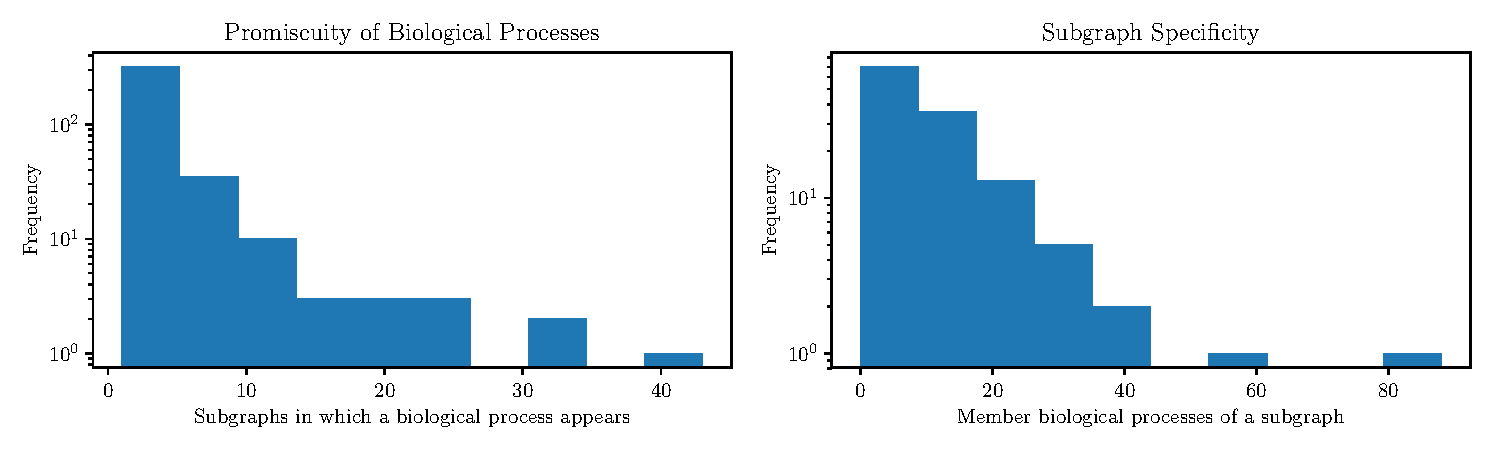
\includegraphics[width=160mm]{images/sg_comparison.pdf}}
\caption[The Landscape of Biological Process Membership in NeuroMMSig Subgraphs]{The landscape of biological process membership shows that there are both biological processes that appear in few and many subgraphs, and subgraphs with few and many biological processes.}
\label{Fig:sg_comparison}
\end{figure}

\begin{figure}
\captionsetup{format=plain}
\makebox[\textwidth]{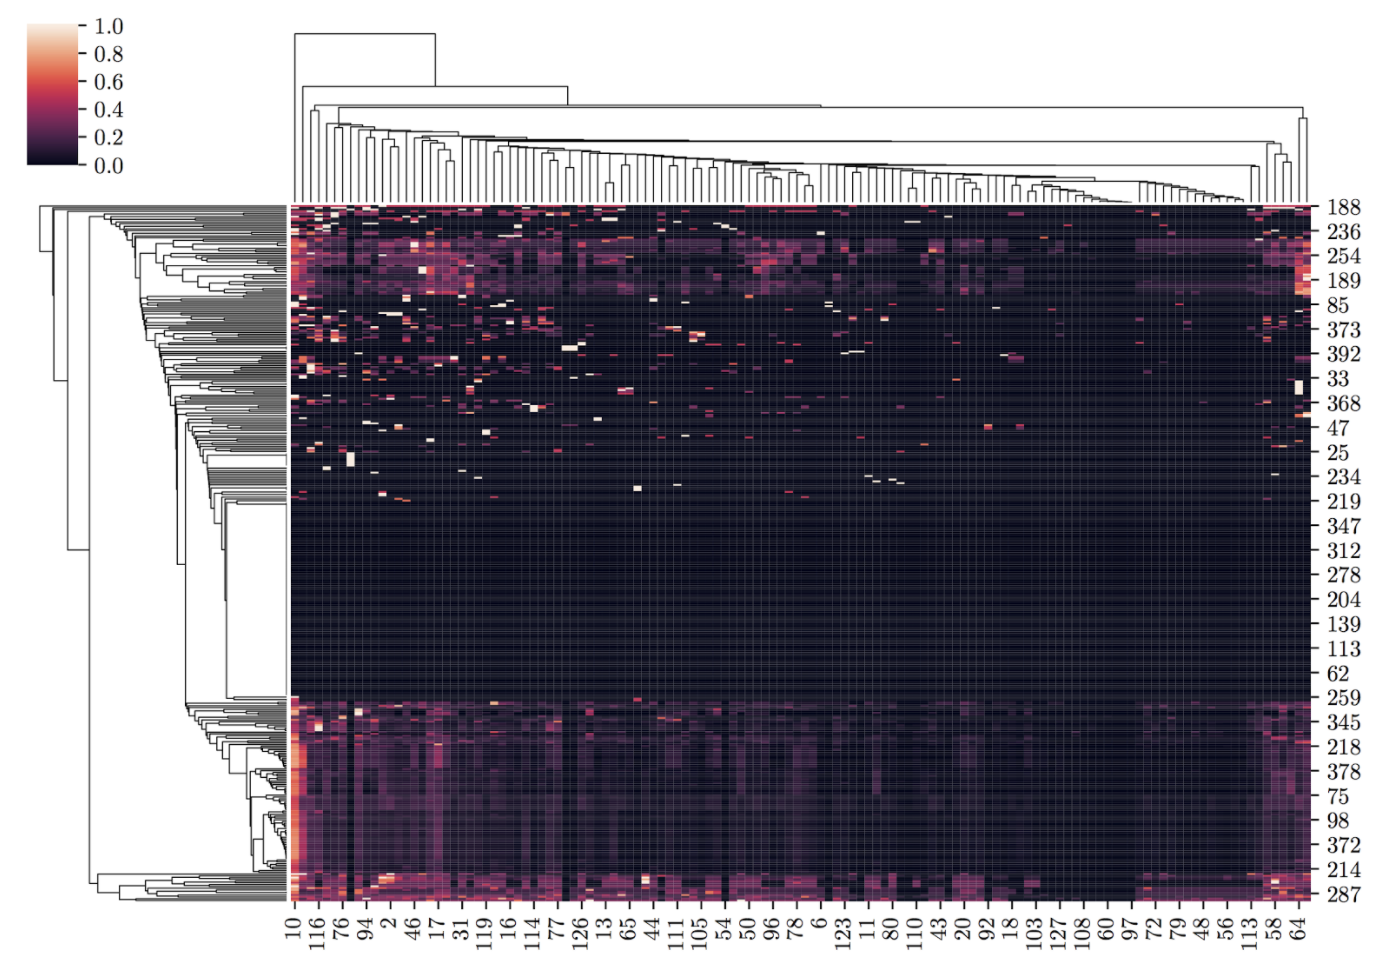
\includegraphics[width=160mm]{images/neurommsig_overlaps.png}}
\caption[Summary of the Overlap of Candidate Mechanisms with NeuroMMSig Subgraphs]{The landscape of candidate mechanism and \ac{NeuroMMSig} overlap, calculated by node overlap. The dark horizontal section directly identifies biological processes that are not annotated in any \ac{NeuroMMSig} subgraphs. This implicates their huge explanatory potential since they are outside the research dogma in Alzheimer's disease research.}
\label{Fig:neurommsig_overlaps}
\end{figure}

This landscape can also be used to annotate new candidate mechanisms to the dogmatic subgraphs in \ac{NeuroMMSig} to allow for more relevant mechanistic analysis. The annotation of further biological processes to subgraphs (Figure 17) can also allow the enrichment strategies in the \ac{NeuroMMSig} Mechanism Enrichment Server to perform enrichment over nodes corresponding to concepts on other scales.

\subsection{Candidate Mechanism Perturbation Amplitude}

All of the previous ideas from this thesis cumulate in the ability to devise and implement an algorithm for data-driven, schema-free analysis of networks. After networks are curated, parsed, enriched, checked for robustness, and triaged into unbiased candidate mechanisms, they can finally be analyzed. This section presents the candidate mechanism perturbation amplitude algorithm. It addresses the issues posed by previous algorithms with more complex randomized approaches and ultimately enables analysis of new modes of data by using a classical schema-free analytical technique similar inspired by other heat diffusion analyses in networks biology \cite{Bernabo2014,Leiserson2015}. The example presented below includes the use of differential gene expression analysis from Alzheimer's disease applied to the unbiased candidate mechanisms generated from the \ac{NeuroMMSig} knowledge assembly.

In this algorithm, heat is applied to the nodes based on the data set. For the differential gene expression experiment, the log-fold-change values were used instead of the corrected p-values to allow for the effects of up- and down-regulation to be admitted in the analysis. Finally, heat diffusion was run with the constraint that decreases edges cause the sign of the heat to be flipped. Because of the construction of unbiased candidate mechanisms, all heat will flow towards their seed biological process nodes. The amount of heat on the biological process node after heat diffusion stops becomes the score for the whole candidate mechanism.

Because heat always flows towards the biological process node, it is possible to remove leaf nodes (nodes with no incoming edges) after each step, since their heat will never change. 

The issue of inconsistent causal networks addressed by the SST algorithm does not affect heat diffusion algorithms since it can quantify multiple conflicting pathways. However, it does not address the possibility of contradictory edges, for example, when A increases B and A decreases B are both true. A random sampling approach is used on networks with contradictory edges and aggregate statistics over multiple trials are used to assess the robustness of the scores as a function of the topology of the underlying candidate mechanisms.

Finally, this algorithm can be tuned to allow the use of correlative relationships. Because many multi-scale and multi-modal data are often measured with correlations to molecular features, this enables experiments to be run using SNP or brain imaging features, whose experiments often measure their correlation with the activity of gene products. 

\subsection{Application Scenario}

This algorithm was applied with the Alzheimer's disease knowledge assembly to assist in interpretation of the differential gene expression experiments from GSE28146 \cite{Blalock2011}. This trial classified patients into three disease progression stages: early, moderate, and severe. While BEL has inherent limits in its temporal expressivity, interpreting data that has an inherent temporal ordering helps overcome this limit. The results for each time point can be accessed at \verb|https://github.com/pybel/pybel-notebooks/blob/master/results/time_series_cmpa.csv|.

\begin{figure}
\captionsetup{format=plain}
\makebox[\textwidth]{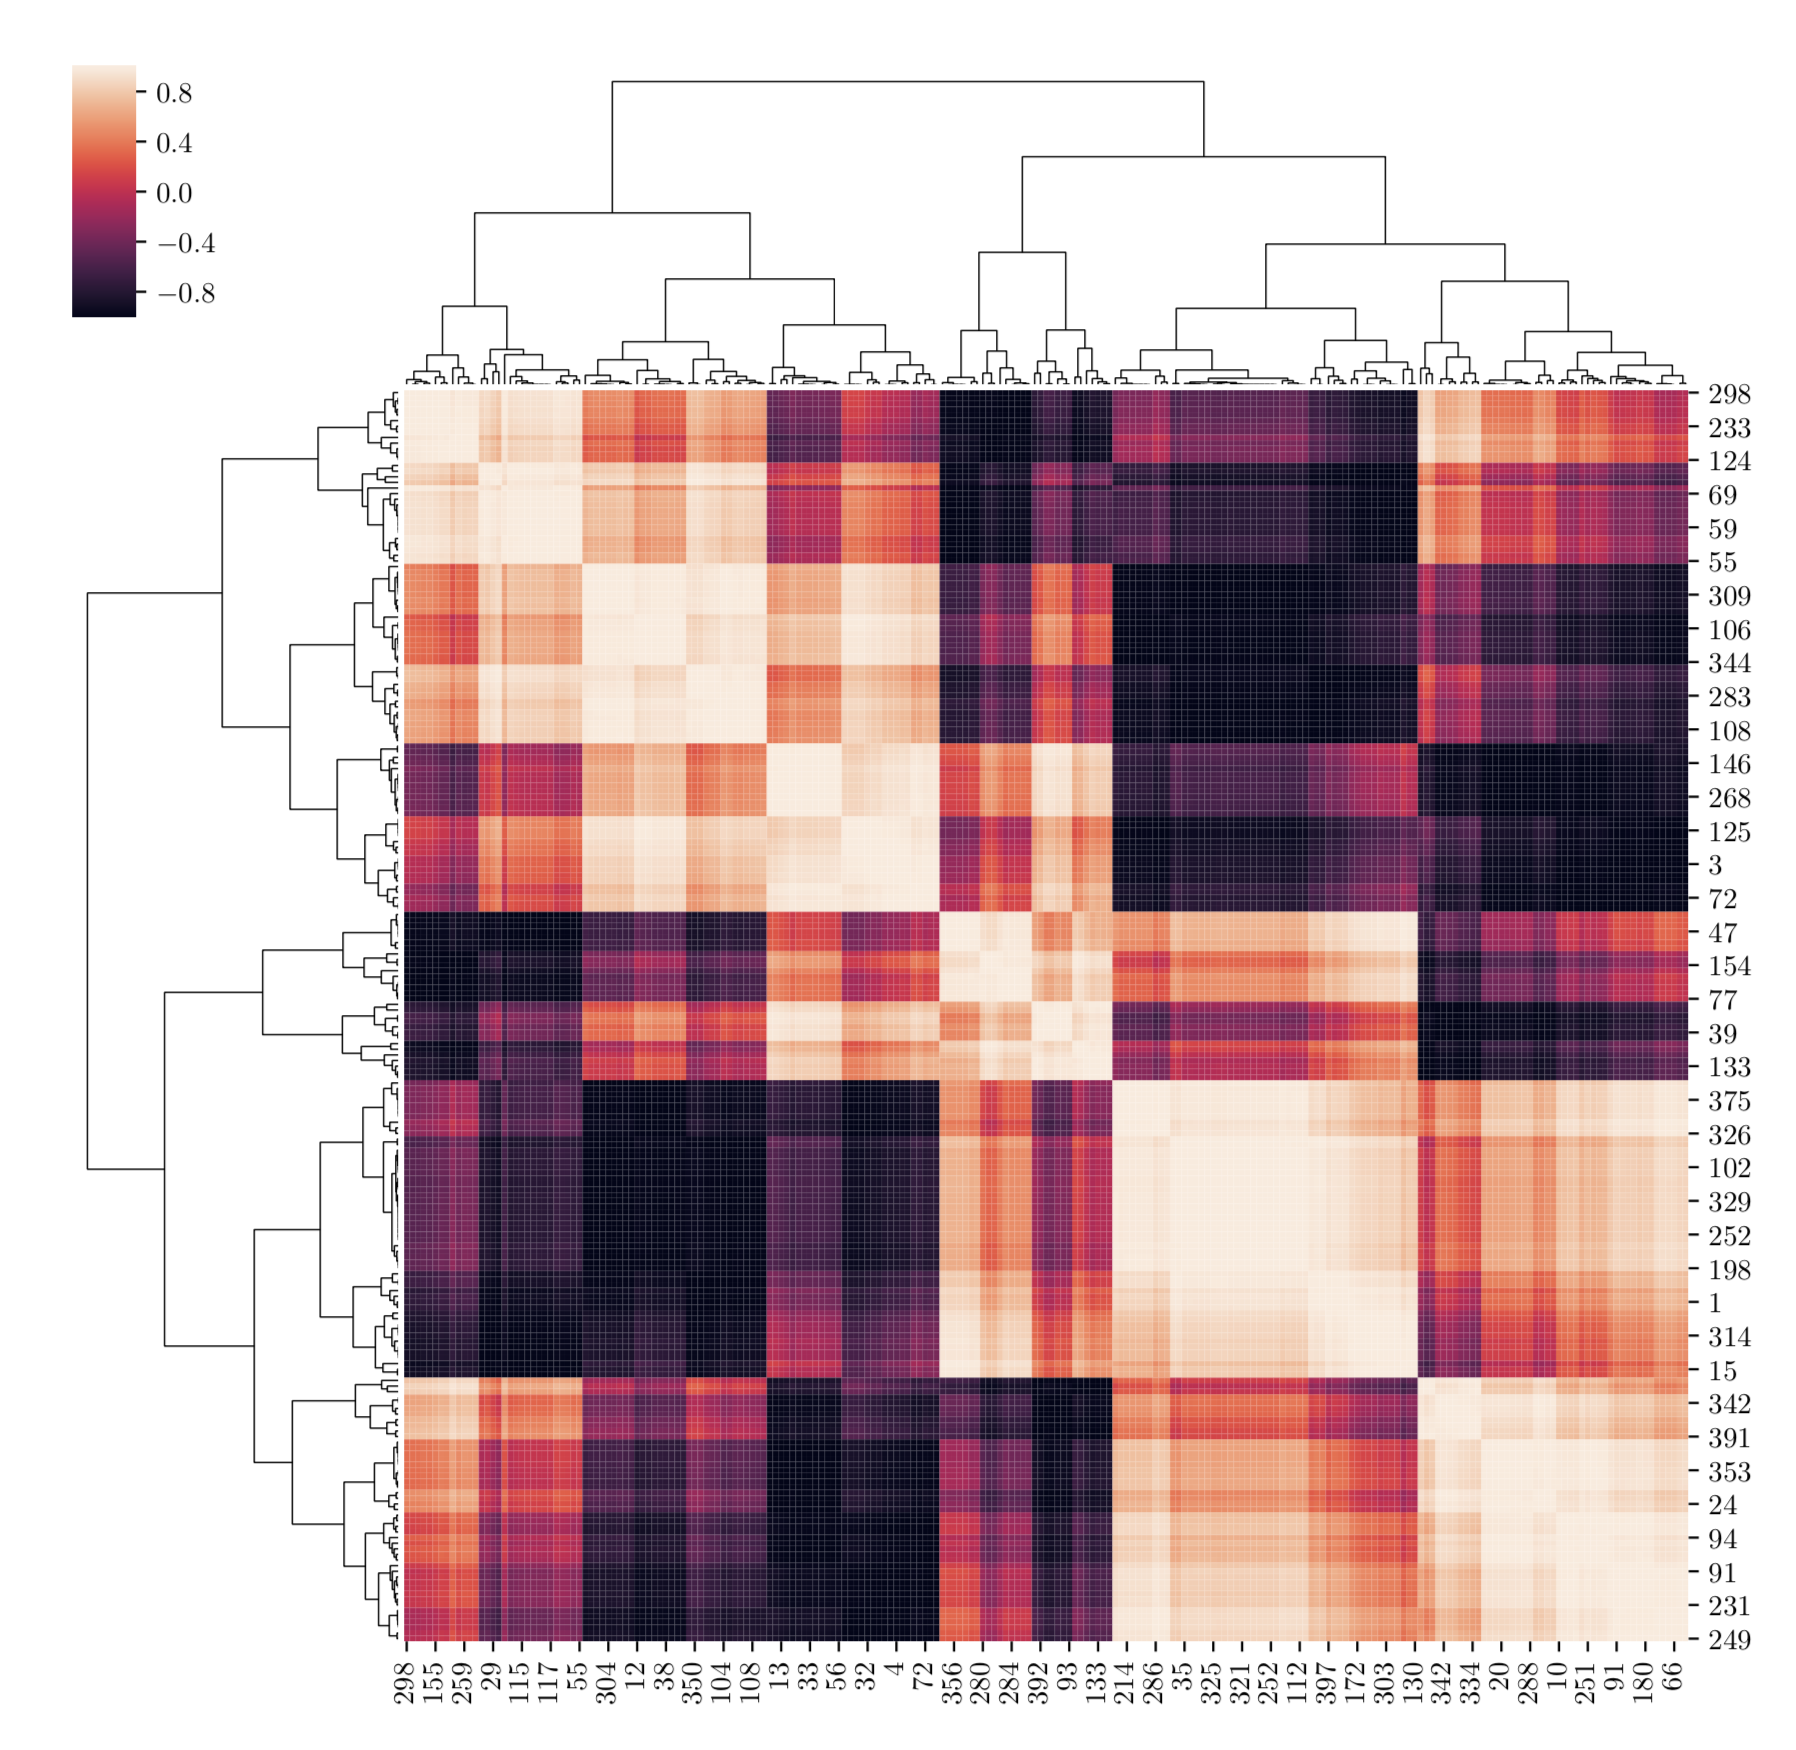
\includegraphics[width=160mm]{images/time_series_clustering.png}}
\caption[Clustering of Time-series Candidate Mechanism Perturbation Amplitude Scores]{A hierarchical clustering over the Pearson correlation of each candidate mechanism score through time suggests there are 4-6 discernible classes.}
\label{Fig:time_series_clustering}
\end{figure}

\begin{figure}
\captionsetup{format=plain}
\makebox[\textwidth]{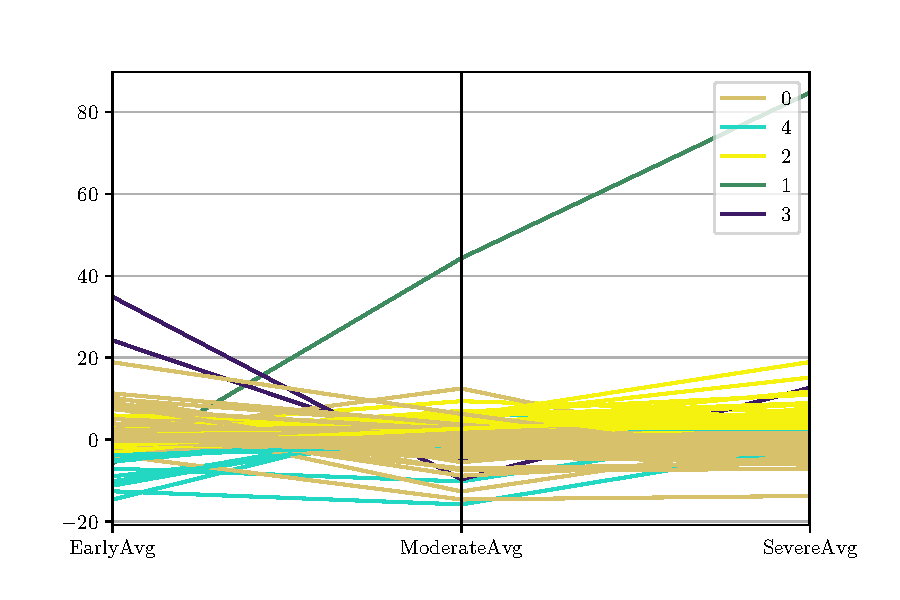
\includegraphics[width=120mm]{images/time_series_pc.pdf}}
\caption[Time-series Candidate Mechanism Perturbation Amplitude Score]{Parallel coordinate plot of all candidate mechanism with coloring by cluster shows the different progressions of biological processes.}
\label{Fig:time_series_pc}
\end{figure}

A hierarchical clustering (Figure 18) was performed using the Pearson correlation coefficient to group biological processes whose observed perturbation changed similarly through time. The dendrogram suggested there were between 4-6 groups of similarly varying processes. In order to make an interpretation, the original values are displayed in a parallel coordinate plot (Figure 19) with colors corresponding to their classes.

In figure 19, class 1 (green) is consists of biological processes that continually increase throughout the progression of the disease. Notably, it contains the inflammatory response. Class 3 (purple) contains biological processes that decrease from the early to moderate stage then increase again. This refers to cell death and neuron death processes. Class 4 includes processes that are initially down-regulated then become less regulated, including mitochondrion-related pathways. Class 2 (yellow) includes processes that do not become disregulated until the severe onset of disease, and have much more variety from glutamate secretion to ion homeostatic processes to metabolic processes. The remaining class does not show significant regulation in any of the disease stages. 

While Alzheimer's disease must be studied with respect to its progression over time, this analysis can provide insight directly to measurements performed on a single time series. Those results provide a ranking that prioritizes the most up- and down-regulated biological processes as a function of the observed data. 


\chapter{Conclusion and outlook}

This master's thesis was originally motivated by the desire to automatically interpret data sets and generate hypotheses using prior knowledge. While working towards that goal, it was necessary to develop an entire computational infrastructure for BEL. That infrastructure was extended with reusable components to integrate prior knowledge from other sources in order to model biology at the finest granularity possible. Next, a framework for testing the validity and robustness of those knowledge assemblies was implemented and applied to the \ac{NeuroMMSig} knowledge base. Finally, algorithms for extracting meaningful subnetworks were applied to enable schema-free and multi-modal analysis using a heat diffusion algorithm. Using this workflow, it is now possible to interpret multi-modal data sets and generate hypotheses in a truly automated fashion.


\printbibliography

\backmatter

\chapter*{Declaration}
I hereby certify that this material is my own work, that I used only those sources and resources referred to in the thesis, and that I have identified citations as such.

\vspace{0.3in}

\noindent Bonn, \today

\vspace{1in}

\noindent Charles Tapley Hoyt

\end{document}
